% Thanks to Project GutenMark
% Source: http://www.sandroid.org/GutenMark/wasftp.GutenMark/MarkedTexts/

\documentclass[12pt,english,oneside]{book}
\usepackage{newcent}
\usepackage[T1]{fontenc}
\usepackage[utf8]{inputenc}
\usepackage[a5paper]{geometry}
\setcounter{secnumdepth}{3}
\setcounter{tocdepth}{3}
\usepackage{graphicx}
\usepackage{hyperref}  % add information to the pdf

\usepackage{type1cm}
\usepackage{lettrine}

\hypersetup{ 
  pdfauthor   = {Sir Arthur Conan Doyle},
  pdfkeywords = {Sherlock Holmes},
  pdftitle    = {Sherlock Holmes 2: The Sign of the Four},
  pdfsubject  = {detective story}
}

\makeatletter
    \newcommand{\noun}[1]{\textsc{#1}}
    \usepackage{babel}
\makeatother
\begin{document}
\sloppy

\evensidemargin = -0.25in

\oddsidemargin = 0.25in

\raggedbottom

\newcommand{\mdsh}[1]{\mbox{#1}\linebreak[1]}

\pagestyle{empty}

\date{}


\title{The Sign of the Four}


\author{Sir Arthur Conan Doyle\\
{\normalsize Illustrated by Richard Gutschmidt}}

\maketitle
\vspace*{\stretch{1}}

\noindent The preparer of this public-domain (U.S.) text is unknown.
However, the Project Gutenberg edition ({}``sign410'') was converted
to \LaTeX{} using \textbf{GutenMark} software and re-edited by Ron
Burkey (formatting only) using \textbf{lyx} software. Report problems
to info@sandroid.org.

\begin{description}
\item [B~12/13/02]Proofing completed.
\item [C~12/30/02]Added illustrations from the 1902 Lutz Verlag (German)
edition, as archived at bakestreet221b.de.
\item [D~01/30/08]{}``----'' was everywhere replaced with {}``---''.
\end{description}
\vspace{\stretch{1}}

\frontmatter


\pagestyle{myheadings} {\footnotesize \tableofcontents{}}\newpage


\mainmatter



\chapter*{\raggedright Chapter I. The Science of Deduction}

\addcontentsline{toc}{chapter}{Chapter I. The Science of Deduction}

\markboth{The Sign of the Four}{The Science of Deduction}

Sherlock Holmes took his bottle from the corner of the mantel-piece
and his hypodermic syringe from its neat morocco case. With his long,
white, nervous fingers he adjusted the delicate needle, and rolled
back his left shirt-cuff. %
\begin{figure}[htbp]
\noindent \begin{center}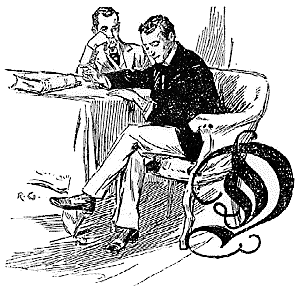
\includegraphics[%
  width=1\columnwidth]{images/sign410-sign-01.png}\end{center}

\noindent \begin{center}\noun{His eyes rested thoughtfully upon
the sinewy forearm and wrist.}\end{center}
\end{figure}
For some little time his eyes rested thoughtfully upon the sinewy
forearm and wrist all dotted and scarred with innumerable puncture-marks.
Finally he thrust the sharp point home, pressed down the tiny piston,
and sank back into the velvet-lined arm-chair with a long sigh of
satisfaction.

Three times a day for many months I had witnessed this performance,
but custom had not reconciled my mind to it. On the contrary, from
day to day I had become more irritable at the sight, and my conscience
swelled nightly within me at the thought that I had lacked the courage
to protest. Again and again I had registered a vow that I should deliver
my soul upon the subject, but there was that in the cool, nonchalant
air of my companion which made him the last man with whom one would
care to take anything approaching to a liberty. His great powers,
his masterly manner, and the experience which I had had of his many
extraordinary qualities, all made me diffident and backward in crossing
him.

Yet upon that afternoon, whether it was the Beaune which I had taken
with my lunch, or the additional exasperation produced by the extreme
deliberation of his manner, I suddenly felt that I could hold out
no longer.

{}``Which is it to-day?''\ I asked,\mdsh{---}``morphine or cocaine?''

He raised his eyes languidly from the old black-letter volume which
he had opened. {}``It is cocaine,'' he said,\mdsh{---}``a seven-per-cent.\ solution.
Would you care to try it?''

{}``No, indeed,'' I answered, brusquely. {}``My constitution has
not got over the Afghan campaign yet. I cannot afford to throw any
extra strain upon it.''

He smiled at my vehemence. {}``Perhaps you are right, Watson,''
he said. {}``I suppose that its influence is physically a bad one.
I find it, however, so transcendently stimulating and clarifying to
the mind that its secondary action is a matter of small moment.''

{}``But consider!''\ I said, earnestly. {}``Count the cost! Your
brain may, as you say, be roused and excited, but it is a pathological
and morbid process, which involves increased tissue-change and may
at last leave a permanent weakness. You know, too, what a black reaction
comes upon you. Surely the game is hardly worth the candle. Why should
you, for a mere passing pleasure, risk the loss of those great powers
with which you have been endowed? Remember that I speak not only as
one comrade to another, but as a medical man to one for whose constitution
he is to some extent answerable.''

He did not seem offended. On the contrary, he put his finger-tips
together and leaned his elbows on the arms of his chair, like one
who has a relish for conversation.

{}``My mind,'' he said, {}``rebels at stagnation. Give me problems,
give me work, give me the most abstruse cryptogram or the most intricate
analysis, and I am in my own proper atmosphere. I can dispense then
with artificial stimulants. But I abhor the dull routine of existence.
I crave for mental exaltation. That is why I have chosen my own particular
profession,\mdsh{---}or rather created it, for I am the only one
in the world.''

{}``The only unofficial detective?'' I said, raising my eyebrows.

{}``The only unofficial consulting detective,'' he answered. {}``I
am the last and highest court of appeal in detection. When Gregson
or Lestrade or Athelney Jones are out of their depths\mdsh{---}which,
by the way, is their normal state\mdsh{---}the matter is laid before
me. I examine the data, as an expert, and pronounce a specialist's
opinion. I claim no credit in such cases. My name figures in no newspaper.
The work itself, the pleasure of finding a field for my peculiar powers,
is my highest reward. But you have yourself had some experience of
my methods of work in the Jefferson Hope case.''

{}``Yes, indeed,'' said I, cordially. {}``I was never so struck
by anything in my life. I even embodied it in a small brochure with
the somewhat fantastic title of `A Study in Scarlet.'''

He shook his head sadly. {}``I glanced over it,'' said he. {}``Honestly,
I cannot congratulate you upon it. Detection is, or ought to be, an
exact science, and should be treated in the same cold and unemotional
manner. You have attempted to tinge it with romanticism, which produces
much the same effect as if you worked a love-story or an elopement
into the fifth proposition of Euclid.''

{}``But the romance was there,'' I remonstrated. {}``I could not
tamper with the facts.''

{}``Some facts should be suppressed, or at least a just sense of
proportion should be observed in treating them. The only point in
the case which deserved mention was the curious analytical reasoning
from effects to causes by which I succeeded in unraveling it.''

I was annoyed at this criticism of a work which had been specially
designed to please him. I confess, too, that I was irritated by the
egotism which seemed to demand that every line of my pamphlet should
be devoted to his own special doings. More than once during the years
that I had lived with him in Baker Street I had observed that a small
vanity underlay my companion's quiet and didactic manner. I made no
remark, however, but sat nursing my wounded leg. I had a Jezail bullet
through it some time before, and, though it did not prevent me from
walking, it ached wearily at every change of the weather.

{}``My practice has extended recently to the Continent,'' said Holmes,
after a while, filling up his old brier-root pipe. {}``I was consulted
last week by Francois Le Villard, who, as you probably know, has come
rather to the front lately in the French detective service. He has
all the Celtic power of quick intuition, but he is deficient in the
wide range of exact knowledge which is essential to the higher developments
of his art. The case was concerned with a will, and possessed some
features of interest. I was able to refer him to two parallel cases,
the one at Riga in 1857, and the other at St.\ Louis in 1871, which
have suggested to him the true solution. Here is the letter which
I had this morning acknowledging my assistance.'' He tossed over,
as he spoke, a crumpled sheet of foreign notepaper. I glanced my eyes
down it, catching a profusion of notes of admiration, with stray {}``\emph{magnifiques},''
{}``\emph{coup-de-maitres},'' and {}``\emph{tours-de-force},''
all testifying to the ardent admiration of the Frenchman.

{}``He speaks as a pupil to his master,'' said I.

{}``Oh, he rates my assistance too highly,'' said Sherlock Holmes,
lightly. {}``He has considerable gifts himself. He possesses two
out of the three qualities necessary for the ideal detective. He has
the power of observation and that of deduction. He is only wanting
in knowledge; and that may come in time. He is now translating my
small works into French.''

{}``Your works?''

{}``Oh, didn't you know?''\ he cried, laughing. {}``Yes, I have
been guilty of several monographs. They are all upon technical subjects.
Here, for example, is one `Upon the Distinction between the Ashes
of the Various Tobaccoes.' In it I enumerate a hundred and forty forms
of cigar-, cigarette-, and pipe-tobacco, with colored plates illustrating
the difference in the ash. It is a point which is continually turning
up in criminal trials, and which is sometimes of supreme importance
as a clue. If you can say definitely, for example, that some murder
has been done by a man who was smoking an Indian \emph{lunkah}, it
obviously narrows your field of search. To the trained eye there is
as much difference between the black ash of a Trichinopoly and the
white fluff of bird's-eye as there is between a cabbage and a potato.''

{}``You have an extraordinary genius for minutiae,'' I remarked.

{}``I appreciate their importance. Here is my monograph upon the
tracing of footsteps, with some remarks upon the uses of plaster of
Paris as a preserver of impresses. Here, too, is a curious little
work upon the influence of a trade upon the form of the hand, with
lithotypes of the hands of slaters, sailors, corkcutters, compositors,
weavers, and diamond-polishers. That is a matter of great practical
interest to the scientific detective,\mdsh{---}especially in cases
of unclaimed bodies, or in discovering the antecedents of criminals.
But I weary you with my hobby.''

{}``Not at all,'' I answered, earnestly. {}``It is of the greatest
interest to me, especially since I have had the opportunity of observing
your practical application of it. But you spoke just now of observation
and deduction. Surely the one to some extent implies the other.''

{}``Why, hardly,'' he answered, leaning back luxuriously in his
arm-chair, and sending up thick blue wreaths from his pipe. {}``For
example, observation shows me that you have been to the Wigmore Street
Post-Office this morning, but deduction lets me know that when there
you dispatched a telegram.''

{}``Right!'' said I. {}``Right on both points! But I confess that
I don't see how you arrived at it. It was a sudden impulse upon my
part, and I have mentioned it to no one.''

{}``It is simplicity itself,'' he remarked, chuckling at my surprise,\mdsh{---}``so
absurdly simple that an explanation is superfluous; and yet it may
serve to define the limits of observation and of deduction. Observation
tells me that you have a little reddish mould adhering to your instep.
Just opposite the Seymour Street Office they have taken up the pavement
and thrown up some earth which lies in such a way that it is difficult
to avoid treading in it in entering. The earth is of this peculiar
reddish tint which is found, as far as I know, nowhere else in the
neighborhood. So much is observation. The rest is deduction.''

{}``How, then, did you deduce the telegram?''

{}``Why, of course I knew that you had not written a letter, since
I sat opposite to you all morning. I see also in your open desk there
that you have a sheet of stamps and a thick bundle of post-cards.
What could you go into the post-office for, then, but to send a wire?
Eliminate all other factors, and the one which remains must be the
truth.''

{}``In this case it certainly is so,'' I replied, after a little
thought. {}``The thing, however, is, as you say, of the simplest.
Would you think me impertinent if I were to put your theories to a
more severe test?''

{}``On the contrary,'' he answered, {}``it would prevent me from
taking a second dose of cocaine. I should be delighted to look into
any problem which you might submit to me.''

{}``I have heard you say that it is difficult for a man to have any
object in daily use without leaving the impress of his individuality
upon it in such a way that a trained observer might read it. Now,
I have here a watch which has recently come into my possession. Would
you have the kindness to let me have an opinion upon the character
or habits of the late owner?''

%
\begin{figure}[htbp]
\noindent \begin{center}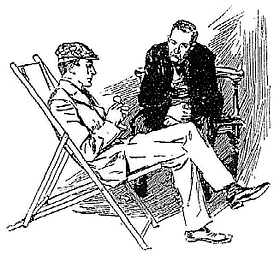
\includegraphics[%
  width=1\columnwidth]{images/sign410-sign-02.png}\end{center}

\noindent \begin{center}\noun{He balanced the watch in his hand.}\end{center}
\end{figure}
I handed him over the watch with some slight feeling of amusement
in my heart, for the test was, as I thought, an impossible one, and
I intended it as a lesson against the somewhat dogmatic tone which
he occasionally assumed. He balanced the watch in his hand, gazed
hard at the dial, opened the back, and examined the works, first with
his naked eyes and then with a powerful convex lens. I could hardly
keep from smiling at his crestfallen face when he finally snapped
the case to and handed it back.

{}``There are hardly any data,'' he remarked. {}``The watch has
been recently cleaned, which robs me of my most suggestive facts.''

{}``You are right,'' I answered. {}``It was cleaned before being
sent to me.'' In my heart I accused my companion of putting forward
a most lame and impotent excuse to cover his failure. What data could
he expect from an uncleaned watch?

{}``Though unsatisfactory, my research has not been entirely barren,''
he observed, staring up at the ceiling with dreamy, lack-lustre eyes.
{}``Subject to your correction, I should judge that the watch belonged
to your elder brother, who inherited it from your father.''

{}``That you gather, no doubt, from the H.\ W.\ upon the back?''

{}``Quite so. The W.\ suggests your own name. The date of the watch
is nearly fifty years back, and the initials are as old as the watch:
so it was made for the last generation. Jewelry usually descents to
the eldest son, and he is most likely to have the same name as the
father. Your father has, if I remember right, been dead many years.
It has, therefore, been in the hands of your eldest brother.''

{}``Right, so far,'' said I. {}``Anything else?''

{}``He was a man of untidy habits,\mdsh{---}very untidy and careless.
He was left with good prospects, but he threw away his chances, lived
for some time in poverty with occasional short intervals of prosperity,
and finally, taking to drink, he died. That is all I can gather.''

I sprang from my chair and limped impatiently about the room with
considerable bitterness in my heart.

{}``This is unworthy of you, Holmes,'' I said. {}``I could not
have believed that you would have descended to this. You have made
inquires into the history of my unhappy brother, and you now pretend
to deduce this knowledge in some fanciful way. You cannot expect me
to believe that you have read all this from his old watch! It is unkind,
and, to speak plainly, has a touch of charlatanism in it.''

{}``My dear doctor,'' said he, kindly, {}``pray accept my apologies.
Viewing the matter as an abstract problem, I had forgotten how personal
and painful a thing it might be to you. I assure you, however, that
I never even know that you had a brother until you handed me the watch.''

{}``Then how in the name of all that is wonderful did you get these
facts? They are absolutely correct in every particular.''

{}``Ah, that is good luck. I could only say what was the balance
of probability. I did not at all expect to be so accurate.''

{}``But it was not mere guess-work?''

{}``No, no: I never guess. It is a shocking habit,\mdsh{---}destructive
to the logical faculty. What seems strange to you is only so because
you do not follow my train of thought or observe the small facts upon
which large inferences may depend. For example, I began by stating
that your brother was careless. When you observe the lower part of
that watch-case you notice that it is not only dinted in two places,
but it is cut and marked all over from the habit of keeping other
hard objects, such as coins or keys, in the same pocket. Surely it
is no great feat to assume that a man who treats a fifty-guinea watch
so cavalierly must be a careless man. Neither is it a very far-fetched
inference that a man who inherits one article of such value is pretty
well provided for in other respects.''

I nodded, to show that I followed his reasoning.

{}``It is very customary for pawnbrokers in England, when they take
a watch, to scratch the number of the ticket with a pin-point upon
the inside of the case. It is more handy than a label, as there is
no risk of the number being lost or transposed. There are no less
than four such numbers visible to my lens on the inside of this case.
Inference,\mdsh{---}that your brother was often at low water. Secondary
inference,\mdsh{---}that he had occasional bursts of prosperity,
or he could not have redeemed the pledge. Finally, I ask you to look
at the inner plate, which contains the key-hole. Look at the thousands
of scratches all round the hole,\mdsh{---}marks where the key has
slipped. What sober man's key could have scored those grooves? But
you will never see a drunkard's watch without them. He winds it at
night, and he leaves these traces of his unsteady hand. Where is the
mystery in all this?''

{}``It is as clear as daylight,'' I answered. {}``I regret the
injustice which I did you. I should have had more faith in your marvellous
faculty. May I ask whether you have any professional inquiry on foot
at present?''

{}``None. Hence the cocaine. I cannot live without brain-work. What
else is there to live for? Stand at the window here. Was ever such
a dreary, dismal, unprofitable world? See how the yellow fog swirls
down the street and drifts across the dun-colored houses. What could
be more hopelessly prosaic and material? What is the use of having
powers, doctor, when one has no field upon which to exert them? Crime
is commonplace, existence is commonplace, and no qualities save those
which are commonplace have any function upon earth.''

I had opened my mouth to reply to this tirade, when with a crisp knock
our landlady entered, bearing a card upon the brass salver.

{}``A young lady for you, sir,'' she said, addressing my companion.

{}``Miss Mary Morstan,'' he read. {}``Hum! I have no recollection
of the name. Ask the young lady to step up, Mrs.\ Hudson. Don't go,
doctor. I should prefer that you remain.''


\chapter*{\raggedright Chapter II. The Statement of the Case}

\addcontentsline{toc}{chapter}{Chapter II. The Statement of the Case}

\markboth{The Sign of the Four}{The Statement of the Case}

Miss Morstan entered the room with a firm step and an outward composure
of manner. She was a blonde young lady, small, dainty, well gloved,
and dressed in the most perfect taste. There was, however, a plainness
and simplicity about her costume which bore with it a suggestion of
limited means. The dress was a sombre grayish beige, untrimmed and
unbraided, and she wore a small turban of the same dull hue, relieved
only by a suspicion of white feather in the side. Her face had neither
regularity of feature nor beauty of complexion, but her expression
was sweet and amiable, and her large blue eyes were singularly spiritual
and sympathetic. In an experience of women which extends over many
nations and three separate continents, I have never looked upon a
face which gave a clearer promise of a refined and sensitive nature.
I could not but observe that as she took the seat which Sherlock Holmes
placed for her, her lip trembled, her hand quivered, and she showed
every sign of intense inward agitation.

{}``I have come to you, Mr.\ Holmes,'' she said, {}``because you
once enabled my employer, Mrs.\ Cecil Forrester, to unravel a little
domestic complication. She was much impressed by your kindness and
skill.''

{}``Mrs.\ Cecil Forrester,'' he repeated thoughtfully. {}``I believe
that I was of some slight service to her. The case, however, as I
remember it, was a very simple one.''

{}``She did not think so. But at least you cannot say the same of
mine. I can hardly imagine anything more strange, more utterly inexplicable,
than the situation in which I find myself.''

%
\begin{figure}[htbp]
\noindent \begin{center}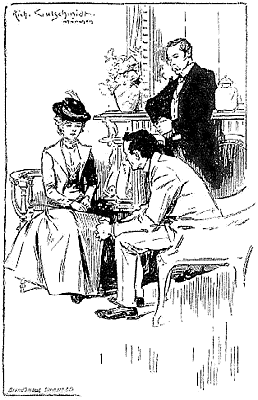
\includegraphics{images/sign410-sign-03.png}\end{center}

\noindent \begin{center}\noun{{}``State your case,'' said he,
in brisk, business tones.}\end{center}
\end{figure}
Holmes rubbed his hands, and his eyes glistened. He leaned forward
in his chair with an expression of extraordinary concentration upon
his clear-cut, hawklike features. {}``State your case,'' said he,
in brisk, business tones.

I felt that my position was an embarrassing one. {}``You will, I
am sure, excuse me,'' I said, rising from my chair.

To my surprise, the young lady held up her gloved hand to detain me.
{}``If your friend,'' she said, {}``would be good enough to stop,
he might be of inestimable service to me.''

I relapsed into my chair.

{}``Briefly,'' she continued, {}``the facts are these. My father
was an officer in an Indian regiment who sent me home when I was quite
a child. My mother was dead, and I had no relative in England. I was
placed, however, in a comfortable boarding establishment at Edinburgh,
and there I remained until I was seventeen years of age. In the year
1878 my father, who was senior captain of his regiment, obtained twelve
months' leave and came home. He telegraphed to me from London that
he had arrived all safe, and directed me to come down at once, giving
the Langham Hotel as his address. His message, as I remember, was
full of kindness and love. On reaching London I drove to the Langham,
and was informed that Captain Morstan was staying there, but that
he had gone out the night before and had not yet returned. I waited
all day without news of him. That night, on the advice of the manager
of the hotel, I communicated with the police, and next morning we
advertised in all the papers. Our inquiries let to no result; and
from that day to this no word has ever been heard of my unfortunate
father. He came home with his heart full of hope, to find some peace,
some comfort, and instead\mbox{----}'' She put her hand to her throat,
and a choking sob cut short the sentence.

{}``The date?''\ asked Holmes, opening his note-book.

{}``He disappeared upon the 3d of December, 1878,\mdsh{---}nearly
ten years ago.''

{}``His luggage?''

{}``Remained at the hotel. There was nothing in it to suggest a clue,\mdsh{---}some
clothes, some books, and a considerable number of curiosities from
the Andaman Islands. He had been one of the officers in charge of
the convict-guard there.''

{}``Had he any friends in town?''

{}``Only one that we know of,\mdsh{---}Major Sholto, of his own
regiment, the 34th Bombay Infantry. The major had retired some little
time before, and lived at Upper Norwood. We communicated with him,
of course, but he did not even know that his brother officer was in
England.''

{}``A singular case,'' remarked Holmes.

{}``I have not yet described to you the most singular part. About
six years ago\mdsh{---}to be exact, upon the 4th of May, 1882\mdsh{---}an
advertisement appeared in the \emph{Times} asking for the address
of Miss Mary Morstan and stating that it would be to her advantage
to come forward. There was no name or address appended. I had at that
time just entered the family of Mrs.\ Cecil Forrester in the capacity
of governess. By her advice I published my address in the advertisement
column. The same day there arrived through the post a small card-board
box addressed to me, which I found to contain a very large and lustrous
pearl. No word of writing was enclosed. Since then every year upon
the same date there has always appeared a similar box, containing
a similar pearl, without any clue as to the sender. They have been
pronounced by an expert to be of a rare variety and of considerable
value. You can see for yourselves that they are very handsome.''
She opened a flat box as she spoke, and showed me six of the finest
pearls that I had ever seen.

{}``Your statement is most interesting,'' said Sherlock Holmes.
{}``Has anything else occurred to you?''

{}``Yes, and no later than to-day. That is why I have come to you.
This morning I received this letter, which you will perhaps read for
yourself.''

{}``Thank you,'' said Holmes. {}``The envelope too, please. Postmark,
London, S.W. Date, July 7. Hum! Man's thumb-mark on corner,\mdsh{---}probably
postman. Best quality paper. Envelopes at sixpence a packet. Particular
man in his stationery. No address. `Be at the third pillar from the
left outside the Lyceum Theatre to-night at seven o'clock. If you
are distrustful, bring two friends. You are a wronged woman, and shall
have justice. Do not bring police. If you do, all will be in vain.
Your unknown friend.' Well, really, this is a very pretty little mystery.
What do you intend to do, Miss Morstan?''

{}``That is exactly what I want to ask you.''

{}``Then we shall most certainly go. You and I and\mdsh{---}yes,
why, Dr.\ Watson is the very man. Your correspondent says two friends.
He and I have worked together before.''

{}``But would he come?''\ she asked, with something appealing in
her voice and expression.

{}``I should be proud and happy,'' said I, fervently, {}``if I
can be of any service.''

{}``You are both very kind,'' she answered. {}``I have led a retired
life, and have no friends whom I could appeal to. If I am here at
six it will do, I suppose?''

{}``You must not be later,'' said Holmes. {}``There is one other
point, however. Is this handwriting the same as that upon the pearl-box
addresses?''

{}``I have them here,'' she answered, producing half a dozen pieces
of paper.

{}``You are certainly a model client. You have the correct intuition.
Let us see, now.'' He spread out the papers upon the table, and gave
little darting glances from one to the other. {}``They are disguised
hands, except the letter,'' he said, presently, {}``but there can
be no question as to the authorship. See how the irrepressible Greek
\emph{e} will break out, and see the twirl of the final \emph{s}.
They are undoubtedly by the same person. I should not like to suggest
false hopes, Miss Morstan, but is there any resemblance between this
hand and that of your father?''

{}``Nothing could be more unlike.''

{}``I expected to hear you say so. We shall look out for you, then,
at six. Pray allow me to keep the papers. I may look into the matter
before then. It is only half-past three. \emph{Au revoir}, then.''

{}``\emph{Au revoir},'' said our visitor, and, with a bright, kindly
glance from one to the other of us, she replaced her pearl-box in
her bosom and hurried away. Standing at the window, I watched her
walking briskly down the street, until the gray turban and white feather
were but a speck in the sombre crowd.

{}``What a very attractive woman!''\ I exclaimed, turning to my
companion.

He had lit his pipe again, and was leaning back with drooping eyelids.
{}``Is she?''\ he said, languidly. {}``I did not observe.''

{}``You really are an automaton,\mdsh{---}a calculating-machine!''\ I
cried. {}``There is something positively inhuman in you at times.''

He smiled gently. {}``It is of the first importance,'' he said,
{}``not to allow your judgment to be biased by personal qualities.
A client is to me a mere unit,\mdsh{---}a factor in a problem. The
emotional qualities are antagonistic to clear reasoning. I assure
you that the most winning woman I ever knew was hanged for poisoning
three little children for their insurance-money, and the most repellant
man of my acquaintance is a philanthropist who has spent nearly a
quarter of a million upon the London poor.''

{}``In this case, however\mdsh{---}''

{}``I never make exceptions. An exception disproves the rule. Have
you ever had occasion to study character in handwriting? What do you
make of this fellow's scribble?''

{}``It is legible and regular,'' I answered. {}``A man of business
habits and some force of character.''

Holmes shook his head. {}``Look at his long letters,'' he said.
{}``They hardly rise above the common herd. That \emph{d} might be
an \emph{a}, and that \emph{l} an \emph{e}. Men of character always
differentiate their long letters, however illegibly they may write.
There is vacillation in his \emph{k}'s and self-esteem in his capitals.
I am going out now. I have some few references to make. Let me recommend
this book,\mdsh{---}one of the most remarkable ever penned. It is
Winwood Reade's `Martyrdom of Man.' I shall be back in an hour.''

I sat in the window with the volume in my hand, but my thoughts were
far from the daring speculations of the writer. My mind ran upon our
late visitor,\mdsh{---}her smiles, the deep rich tones of her voice,
the strange mystery which overhung her life. If she were seventeen
at the time of her father's disappearance she must be seven-and-twenty
now,\mdsh{---}a sweet age, when youth has lost its self-consciousness
and become a little sobered by experience. So I sat and mused, until
such dangerous thoughts came into my head that I hurried away to my
desk and plunged furiously into the latest treatise upon pathology.
What was I, an army surgeon with a weak leg and a weaker banking-account,
that I should dare to think of such things? She was a unit, a factor,\mdsh{---}nothing
more. If my future were black, it was better surely to face it like
a man than to attempt to brighten it by mere will-o'-the-wisps of
the imagination.


\chapter*{\raggedright Chapter III. In Quest of a Solution}

\addcontentsline{toc}{chapter}{Chapter III. In Quest of a Solution}

\markboth{The Sign of the Four}{In Quest of a Solution}

It was half-past five before Holmes returned. He was bright, eager,
and in excellent spirits,\mdsh{---}a mood which in his case alternated
with fits of the blackest depression.

{}``There is no great mystery in this matter,'' he said, taking
the cup of tea which I had poured out for him. {}``The facts appear
to admit of only one explanation.''

{}``What! you have solved it already?''

{}``Well, that would be too much to say. I have discovered a suggestive
fact, that is all. It is, however, \textit{very} suggestive. The details
are still to be added. I have just found, on consulting the back files
of the \emph{Times}, that Major Sholto, of Upper Norword, late of
the 34th Bombay Infantry, died upon the 28th of April, 1882.''

{}``I may be very obtuse, Holmes, but I fail to see what this suggests.''

{}``No? You surprise me. Look at it in this way, then. Captain Morstan
disappears. The only person in London whom he could have visited is
Major Sholto. Major Sholto denies having heard that he was in London.
Four years later Sholto dies. \textit{Within} \emph{a} \textit{week}
\textit{of} \textit{his} \textit{death} Captain Morstan's daughter
receives a valuable present, which is repeated from year to year,
and now culminates in a letter which describes her as a wronged woman.
What wrong can it refer to except this deprivation of her father?
And why should the presents begin immediately after Sholto's death,
unless it is that Sholto's heir knows something of the mystery and
desires to make compensation? Have you any alternative theory which
will meet the facts?''

{}``But what a strange compensation! And how strangely made! Why,
too, should he write a letter now, rather than six years ago? Again,
the letter speaks of giving her justice. What justice can she have?
It is too much to suppose that her father is still alive. There is
no other injustice in her case that you know of.''

{}``There are difficulties; there are certainly difficulties,''
said Sherlock Holmes, pensively. {}``But our expedition of to-night
will solve them all. Ah, here is a four-wheeler, and Miss Morstan
is inside. Are you all ready? Then we had better go down, for it is
a little past the hour.''

I picked up my hat and my heaviest stick, but I observed that Holmes
took his revolver from his drawer and slipped it into his pocket.
It was clear that he thought that our night's work might be a serious
one.

Miss Morstan was muffled in a dark cloak, and her sensitive face was
composed, but pale. She must have been more than woman if she did
not feel some uneasiness at the strange enterprise upon which we were
embarking, yet her self-control was perfect, and she readily answered
the few additional questions which Sherlock Holmes put to her.

{}``Major Sholto was a very particular friend of papa's,'' she said.
{}``His letters were full of allusions to the major. He and papa
were in command of the troops at the Andaman Islands, so they were
thrown a great deal together. By the way, a curious paper was found
in papa's desk which no one could understand. I don't suppose that
it is of the slightest importance, but I thought you might care to
see it, so I brought it with me. It is here.''

Holmes unfolded the paper carefully and smoothed it out upon his knee.
He then very methodically examined it all over with his double lens.

{}``It is paper of native Indian manufacture,'' he remarked. {}``It
has at some time been pinned to a board. The diagram upon it appears
to be a plan of part of a large building with numerous halls, corridors,
and passages. At one point is a small cross done in red ink, and above
it is `3.37 from left,' in faded pencil-writing. In the left-hand
corner is a curious hieroglyphic like four crosses in a line with
their arms touching. Beside it is written, in very rough and coarse
characters, `The sign of the four,\mdsh{---}Jonathan Small, Mahomet
Singh, Abdullah Khan, Dost Akbar.' No, I confess that I do not see
how this bears upon the matter. Yet it is evidently a document of
importance. It has been kept carefully in a pocket-book; for the one
side is as clean as the other.''

{}``It was in his pocket-book that we found it.''

{}``Preserve it carefully, then, Miss Morstan, for it may prove to
be of use to us. I begin to suspect that this matter may turn out
to be much deeper and more subtle than I at first supposed. I must
reconsider my ideas.'' He leaned back in the cab, and I could see
by his drawn brow and his vacant eye that he was thinking intently.
Miss Morstan and I chatted in an undertone about our present expedition
and its possible outcome, but our companion maintained his impenetrable
reserve until the end of our journey.

It was a September evening, and not yet seven o'clock, but the day
had been a dreary one, and a dense drizzly fog lay low upon the great
city. Mud-colored clouds drooped sadly over the muddy streets. Down
the Strand the lamps were but misty splotches of diffused light which
threw a feeble circular glimmer upon the slimy pavement. The yellow
glare from the shop-windows streamed out into the steamy, vaporous
air, and threw a murky, shifting radiance across the crowded thoroughfare.
There was, to my mind, something eerie and ghost-like in the endless
procession of faces which flitted across these narrow bars of light,\mdsh{---}sad
faces and glad, haggard and merry. Like all human kind, they flitted
from the gloom into the light, and so back into the gloom once more.
I am not subject to impressions, but the dull, heavy evening, with
the strange business upon which we were engaged, combined to make
me nervous and depressed. I could see from Miss Morstan's manner that
she was suffering from the same feeling. Holmes alone could rise superior
to petty influences. He held his open note-book upon his knee, and
from time to time he jotted down figures and memoranda in the light
of his pocket-lantern.

%
\begin{figure}[htbp]
\noindent \begin{center}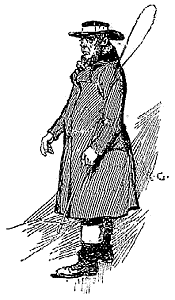
\includegraphics{images/sign410-sign-04.png}\end{center}

\noindent \begin{center}\noun{A small, dark, brisk man in the dress
of a coachman.}\end{center}
\end{figure}
At the Lyceum Theatre the crowds were already thick at the side-entrances.
In front a continuous stream of hansoms and four-wheelers were rattling
up, discharging their cargoes of shirt-fronted men and beshawled,
bediamonded women. We had hardly reached the third pillar, which was
our rendezvous, before a small, dark, brisk man in the dress of a
coachman accosted us.

{}``Are you the parties who come with Miss Morstan?'' he asked.

{}``I am Miss Morstan, and these two gentlemen are my friends,''
said she.

He bent a pair of wonderfully penetrating and questioning eyes upon
us. {}``You will excuse me, miss,'' he said with a certain dogged
manner, {}``but I was to ask you to give me your word that neither
of your companions is a police-officer.''

{}``I give you my word on that,'' she answered.

He gave a shrill whistle, on which a street Arab led across a four-wheeler
and opened the door. The man who had addressed us mounted to the box,
while we took our places inside. We had hardly done so before the
driver whipped up his horse, and we plunged away at a furious pace
through the foggy streets.

The situation was a curious one. We were driving to an unknown place,
on an unknown errand. Yet our invitation was either a complete hoax,\mdsh{---}which
was an inconceivable hypothesis,\mdsh{---}or else we had good reason
to think that important issues might hang upon our journey. Miss Morstan's
demeanor was as resolute and collected as ever. I endeavored to cheer
and amuse her by reminiscences of my adventures in Afghanistan; but,
to tell the truth, I was myself so excited at our situation and so
curious as to our destination that my stories were slightly involved.
To this day she declares that I told her one moving anecdote as to
how a musket looked into my tent at the dead of night, and how I fired
a double-barrelled tiger cub at it. At first I had some idea as to
the direction in which we were driving; but soon, what with our pace,
the fog, and my own limited knowledge of London, I lost my bearings,
and knew nothing, save that we seemed to be going a very long way.
Sherlock Holmes was never at fault, however, and he muttered the names
as the cab rattled through squares and in and out by tortuous by-streets.

{}``Rochester Row,'' said he. {}``Now Vincent Square. Now we come
out on the Vauxhall Bridge Road. We are making for the Surrey side,
apparently. Yes, I thought so. Now we are on the bridge. You can catch
glimpses of the river.''

We did indeed bet a fleeting view of a stretch of the Thames with
the lamps shining upon the broad, silent water; but our cab dashed
on, and was soon involved in a labyrinth of streets upon the other
side.

{}``Wordsworth Road,'' said my companion. {}``Priory Road. Lark
Hall Lane. Stockwell Place. Robert Street. Cold Harbor Lane. Our quest
does not appear to take us to very fashionable regions.''

We had, indeed, reached a questionable and forbidding neighborhood.
Long lines of dull brick houses were only relieved by the coarse glare
and tawdry brilliancy of public houses at the corner. Then came rows
of two-storied villas each with a fronting of miniature garden, and
then again interminable lines of new staring brick buildings,\mdsh{---}the
monster tentacles which the giant city was throwing out into the country.
At last the cab drew up at the third house in a new terrace. None
of the other houses were inhabited, and that at which we stopped was
as dark as its neighbors, save for a single glimmer in the kitchen
window. On our knocking, however, the door was instantly thrown open
by a Hindoo servant clad in a yellow turban, white loose-fitting clothes,
and a yellow sash. There was something strangely incongruous in this
Oriental figure framed in the commonplace door-way of a third-rate
suburban dwelling-house.

{}``The Sahib awaits you,'' said he, and even as he spoke there
came a high piping voice from some inner room. {}``Show them in to
me, \emph{khitmutgar},'' it cried. {}``Show them straight in to
me.''


\chapter*{\raggedright Chapter IV. The Story of the Bald-Headed Man}

\addcontentsline{toc}{chapter}{Chapter IV. The Story of the Bald-Headed\\
Man}

\markboth{The Sign of the Four}{The Story of the Bald-Headed Man}

We followed the Indian down a sordid and common passage, ill lit and
worse furnished, until he came to a door upon the right, which he
threw open. A blaze of yellow light streamed out upon us, and in the
centre of the glare there stood a small man with a very high head,
a bristle of red hair all round the fringe of it, and a bald, shining
scalp which shot out from among it like a mountain-peak from fir-trees.
He writhed his hands together as he stood, and his features were in
a perpetual jerk, now smiling, now scowling, but never for an instant
in repose. Nature had given him a pendulous lip, and a too visible
line of yellow and irregular teeth, which he strove feebly to conceal
by constantly passing his hand over the lower part of his face. In
spite of his obtrusive baldness, he gave the impression of youth.
In point of fact he had just turned his thirtieth year.

{}``Your servant, Miss Morstan,'' he kept repeating, in a thin,
high voice. {}``Your servant, gentlemen. Pray step into my little
sanctum. A small place, miss, but furnished to my own liking. An oasis
of art in the howling desert of South London.''

We were all astonished by the appearance of the apartment into which
he invited us. In that sorry house it looked as out of place as a
diamond of the first water in a setting of brass. The richest and
glossiest of curtains and tapestries draped the walls, looped back
here and there to expose some richly-mounted painting or Oriental
vase. The carpet was of amber-and-black, so soft and so thick that
the foot sank pleasantly into it, as into a bed of moss. Two great
tiger-skins thrown athwart it increased the suggestion of Eastern
luxury, as did a huge hookah which stood upon a mat in the corner.
A lamp in the fashion of a silver dove was hung from an almost invisible
golden wire in the centre of the room. As it burned it filled the
air with a subtle and aromatic odor.

{}``Mr.\ Thaddeus Sholto,'' said the little man, still jerking
and smiling. {}``That is my name. You are Miss Morstan, of course.
And these gentlemen\mdsh{---}''

{}``This is Mr.\ Sherlock Holmes, and this is Dr.\ Watson.''

{}``A doctor, eh?''\ cried he, much excited. {}``Have you your
stethoscope? Might I ask you\mdsh{---}would you have the kindness?
I have grave doubts as to my mitral valve, if you would be so very
good. The aortic I may rely upon, but I should value your opinion
upon the mitral.''

I listened to his heart, as requested, but was unable to find anything
amiss, save indeed that he was in an ecstasy of fear, for he shivered
from head to foot. {}``It appears to be normal,'' I said. {}``You
have no cause for uneasiness.''

{}``You will excuse my anxiety, Miss Morstan,'' he remarked, airily.
{}``I am a great sufferer, and I have long had suspicions as to that
valve. I am delighted to hear that they are unwarranted. Had your
father, Miss Morstan, refrained from throwing a strain upon his heart,
he might have been alive now.''

I could have struck the man across the face, so hot was I at this
callous and off-hand reference to so delicate a matter. Miss Morstan
sat down, and her face grew white to the lips. {}``I knew in my heart
that he was dead,'' said she.

{}``I can give you every information,'' said he, {}``and, what
is more, I can do you justice; and I will, too, whatever Brother Bartholomew
may say. I am so glad to have your friends here, not only as an escort
to you, but also as witnesses to what I am about to do and say. The
three of us can show a bold front to Brother Bartholomew. But let
us have no outsiders,\mdsh{---}no police or officials. We can settle
everything satisfactorily among ourselves, without any interference.
Nothing would annoy Brother Bartholomew more than any publicity.''
He sat down upon a low settee and blinked at us inquiringly with his
weak, watery blue eyes.

{}``For my part,'' said Holmes, {}``whatever you may choose to
say will go no further.''

I nodded to show my agreement.

{}``That is well! That is well!'' said he. {}``May I offer you
a glass of Chianti, Miss Morstan? Or of Tokay? I keep no other wines.
Shall I open a flask? No? Well, then, I trust that you have no objection
to tobacco-smoke, to the mild balsamic odor of the Eastern tobacco.
I am a little nervous, and I find my hookah an invaluable sedative.''
He applied a taper to the great bowl, and the smoke bubbled merrily
through the rose-water. We sat all three in a semicircle, with our
heads advanced, and our chins upon our hands, while the strange, jerky
little fellow, with his high, shining head, puffed uneasily in the
centre.

{}``When I first determined to make this communication to you,''
said he, {}``I might have given you my address, but I feared that
you might disregard my request and bring unpleasant people with you.
I took the liberty, therefore, of making an appointment in such a
way that my man Williams might be able to see you first. I have complete
confidence in his discretion, and he had orders, if he were dissatisfied,
to proceed no further in the matter. You will excuse these precautions,
but I am a man of somewhat retiring, and I might even say refined,
tastes, and there is nothing more un\ae sthetic than a policeman.
I have a natural shrinking from all forms of rough materialism. I
seldom come in contact with the rough crowd. I live, as you see, with
some little atmosphere of elegance around me. I may call myself a
patron of the arts. It is my weakness. The landscape is a genuine
Corot, and, though a connoisseur might perhaps throw a doubt upon
that Salvator Rosa, there cannot be the least question about the Bouguereau.
I am partial to the modern French school.''

{}``You will excuse me, Mr.\ Sholto,'' said Miss Morstan, {}``but
I am here at your request to learn something which you desire to tell
me. It is very late, and I should desire the interview to be as short
as possible.''

{}``At the best it must take some time,'' he answered; {}``for
we shall certainly have to go to Norwood and see Brother Bartholomew.
We shall all go and try if we can get the better of Brother Bartholomew.
He is very angry with me for taking the course which has seemed right
to me. I had quite high words with him last night. You cannot imagine
what a terrible fellow he is when he is angry.''

{}``If we are to go to Norwood it would perhaps be as well to start
at once,'' I ventured to remark.

He laughed until his ears were quite red. {}``That would hardly do,''
he cried. {}``I don't know what he would say if I brought you in
that sudden way. No, I must prepare you by showing you how we all
stand to each other. In the first place, I must tell you that there
are several points in the story of which I am myself ignorant. I can
only lay the facts before you as far as I know them myself.

{}``My father was, as you may have guessed, Major John Sholto, once
of the Indian army. He retired some eleven years ago, and came to
live at Pondicherry Lodge in Upper Norwood. He had prospered in India,
and brought back with him a considerable sum of money, a large collection
of valuable curiosities, and a staff of native servants. With these
advantages he bought himself a house, and lived in great luxury. My
twin-brother Bartholomew and I were the only children.

{}``I very well remember the sensation which was caused by the disappearance
of Captain Morstan. We read the details in the papers, and, knowing
that he had been a friend of our father's, we discussed the case freely
in his presence. He used to join in our speculations as to what could
have happened. Never for an instant did we suspect that he had the
whole secret hidden in his own breast,\mdsh{---}that of all men he
alone knew the fate of Arthur Morstan.

{}``We did know, however, that some mystery\mdsh{---}some positive
danger\mdsh{---}overhung our father. He was very fearful of going
out alone, and he always employed two prize-fighters to act as porters
at Pondicherry Lodge. Williams, who drove you to-night, was one of
them. He was once light-weight champion of England. Our father would
never tell us what it was he feared, but he had a most marked aversion
to men with wooden legs. On one occasion he actually fired his revolver
at a wooden-legged man, who proved to be a harmless tradesman canvassing
for orders. We had to pay a large sum to hush the matter up. My brother
and I used to think this a mere whim of my father's, but events have
since led us to change our opinion.

{}``Early in 1882 my father received a letter from India which was
a great shock to him. He nearly fainted at the breakfast-table when
he opened it, and from that day he sickened to his death. What was
in the letter we could never discover, but I could see as he held
it that it was short and written in a scrawling hand. He had suffered
for years from an enlarged spleen, but he now became rapidly worse,
and towards the end of April we were informed that he was beyond all
hope, and that he wished to make a last communication to us.

{}``When we entered his room he was propped up with pillows and breathing
heavily. He besought us to lock the door and to come upon either side
of the bed. Then, grasping our hands, he made a remarkable statement
to us, in a voice which was broken as much by emotion as by pain.
I shall try and give it to you in his own very words.

{}```I have only one thing,' he said, `which weighs upon my mind
at this supreme moment. It is my treatment of poor Morstan's orphan.
The cursed greed which has been my besetting sin through life has
withheld from her the treasure, half at least of which should have
been hers. And yet I have made no use of it myself,\mdsh{---}so blind
and foolish a thing is avarice. The mere feeling of possession has
been so dear to me that I could not bear to share it with another.
See that chaplet dipped with pearls beside the quinine-bottle. Even
that I could not bear to part with, although I had got it out with
the design of sending it to her. You, my sons, will give her a fair
share of the Agra treasure. But send her nothing\mdsh{---}not even
the chaplet\mdsh{---}until I am gone. After all, men have been as
bad as this and have recovered.

%
\begin{figure}[htbp]
\noindent \begin{center}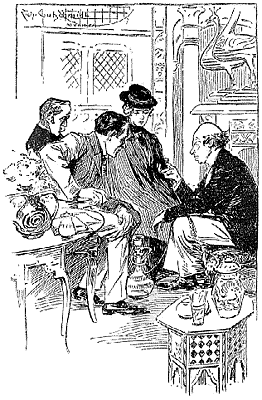
\includegraphics{images/sign410-sign-05.png}\end{center}

\noindent \begin{center}\noun{`I will tell you how Morstan died,'
he continued.}\end{center}
\end{figure}
{}```I will tell you how Morstan died,' he continued. `He had suffered
for years from a weak heart, but he concealed it from every one. I
alone knew it. When in India, he and I, through a remarkable chain
of circumstances, came into possession of a considerable treasure.
I brought it over to England, and on the night of Morstan's arrival
he came straight over here to claim his share. He walked over from
the station, and was admitted by my faithful Lal Chowdar, who is now
dead. Morstan and I had a difference of opinion as to the division
of the treasure, and we came to heated words. Morstan had sprung out
of his chair in a paroxysm of anger, when he suddenly pressed his
hand to his side, his face turned a dusky hue, and he fell backwards,
cutting his head against the corner of the treasure-chest. When I
stooped over him I found, to my horror, that he was dead.

{}```For a long time I sat half distracted, wondering what I should
do. My first impulse was, of course, to call for assistance; but I
could not but recognize that there was every chance that I would be
accused of his murder. His death at the moment of a quarrel, and the
gash in his head, would be black against me. Again, an official inquiry
could not be made without bringing out some facts about the treasure,
which I was particularly anxious to keep secret. He had told me that
no soul upon earth knew where he had gone. There seemed to be no necessity
why any soul ever should know.

{}```I was still pondering over the matter, when, looking up, I saw
my servant, Lal Chowdar, in the doorway. He stole in and bolted the
door behind him. {}``Do not fear, Sahib,'' he said. {}``No one
need know that you have killed him. Let us hide him away, and who
is the wiser?'' {}``I did not kill him,'' said I.\  Lal Chowdar
shook his head and smiled. {}``I heard it all, Sahib,'' said he.
{}``I heard you quarrel, and I heard the blow. But my lips are sealed.
All are asleep in the house. Let us put him away together.'' That
was enough to decide me. If my own servant could not believe my innocence,
how could I hope to make it good before twelve foolish tradesmen in
a jury-box? Lal Chowdar and I disposed of the body that night, and
within a few days the London papers were full of the mysterious disappearance
of Captain Morstan. You will see from what I say that I can hardly
be blamed in the matter. My fault lies in the fact that we concealed
not only the body, but also the treasure, and that I have clung to
Morstan's share as well as to my own. I wish you, therefore, to make
restitution. Put your ears down to my mouth. The treasure is hidden
in\mdsh{---}' At this instant a horrible change came over his expression;
his eyes stared wildly, his jaw dropped, and he yelled, in a voice
which I can never forget, `Keep him out! For Christ's sake keep him
out!' We both stared round at the window behind us upon which his
gaze was fixed. A face was looking in at us out of the darkness. We
could see the whitening of the nose where it was pressed against the
glass. It was a bearded, hairy face, with wild cruel eyes and an expression
of concentrated malevolence. My brother and I rushed towards the window,
but the man was gone. When we returned to my father his head had dropped
and his pulse had ceased to beat.

{}``We searched the garden that night, but found no sign of the intruder,
save that just under the window a single footmark was visible in the
flower-bed. But for that one trace, we might have thought that our
imaginations had conjured up that wild, fierce face. We soon, however,
had another and a more striking proof that there were secret agencies
at work all round us. The window of my father's room was found open
in the morning, his cupboards and boxes had been rifled, and upon
his chest was fixed a torn piece of paper, with the words `The sign
of the four' scrawled across it. What the phrase meant, or who our
secret visitor may have been, we never knew. As far as we can judge,
none of my father's property had been actually stolen, though everything
had been turned out. My brother and I naturally associated this peculiar
incident with the fear which haunted my father during his life; but
it is still a complete mystery to us.''

The little man stopped to relight his hookah and puffed thoughtfully
for a few moments. We had all sat absorbed, listening to his extraordinary
narrative. At the short account of her father's death Miss Morstan
had turned deadly white, and for a moment I feared that she was about
to faint. She rallied however, on drinking a glass of water which
I quietly poured out for her from a Venetian carafe upon the side-table.
Sherlock Holmes leaned back in his chair with an abstracted expression
and the lids drawn low over his glittering eyes. As I glanced at him
I could not but think how on that very day he had complained bitterly
of the commonplaceness of life. Here at least was a problem which
would tax his sagacity to the utmost. Mr.\ Thaddeus Sholto looked
from one to the other of us with an obvious pride at the effect which
his story had produced, and then continued between the puffs of his
overgrown pipe.

{}``My brother and I,'' said he, {}``were, as you may imagine,
much excited as to the treasure which my father had spoken of. For
weeks and for months we dug and delved in every part of the garden,
without discovering its whereabouts. It was maddening to think that
the hiding-place was on his very lips at the moment that he died.
We could judge the splendor of the missing riches by the chaplet which
he had taken out. Over this chaplet my brother Bartholomew and I had
some little discussion. The pearls were evidently of great value,
and he was averse to part with them, for, between friends, my brother
was himself a little inclined to my father's fault. He thought, too,
that if we parted with the chaplet it might give rise to gossip and
finally bring us into trouble. It was all that I could do to persuade
him to let me find out Miss Morstan's address and send her a detached
pearl at fixed intervals, so that at least she might never feel destitute.''

{}``It was a kindly thought,'' said our companion, earnestly. {}``It
was extremely good of you.''

The little man waved his hand deprecatingly. {}``We were your trustees,''
he said. {}``That was the view which I took of it, though Brother
Bartholomew could not altogether see it in that light. We had plenty
of money ourselves. I desired no more. Besides, it would have been
such bad taste to have treated a young lady in so scurvy a fashion.
`\emph{Le mauvais gout mene au crime}.' The French have a very neat
way of putting these things. Our difference of opinion on this subject
went so far that I thought it best to set up rooms for myself: so
I left Pondicherry Lodge, taking the old \emph{khitmutgar} and Williams
with me. Yesterday, however, I learn that an event of extreme importance
has occurred. The treasure has been discovered. I instantly communicated
with Miss Morstan, and it only remains for us to drive out to Norwood
and demand our share. I explained my views last night to Brother Bartholomew:
so we shall be expected, if not welcome, visitors.''

Mr.\ Thaddeus Sholto ceased, and sat twitching on his luxurious settee.
We all remained silent, with our thoughts upon the new development
which the mysterious business had taken. Holmes was the first to spring
to his feet.

{}``You have done well, sir, from first to last,'' said he. {}``It
is possible that we may be able to make you some small return by throwing
some light upon that which is still dark to you. But, as Miss Morstan
remarked just now, it is late, and we had best put the matter through
without delay.''

Our new acquaintance very deliberately coiled up the tube of his hookah,
and produced from behind a curtain a very long befrogged topcoat with
Astrakhan collar and cuffs. This he buttoned tightly up, in spite
of the extreme closeness of the night, and finished his attire by
putting on a rabbit-skin cap with hanging lappets which covered the
ears, so that no part of him was visible save his mobile and peaky
face. {}``My health is somewhat fragile,'' he remarked, as he led
the way down the passage. {}``I am compelled to be a valetudinarian.''

Our cab was awaiting us outside, and our programme was evidently prearranged,
for the driver started off at once at a rapid pace. Thaddeus Sholto
talked incessantly, in a voice which rose high above the rattle of
the wheels.

{}``Bartholomew is a clever fellow,'' said he. {}``How do you think
he found out where the treasure was? He had come to the conclusion
that it was somewhere indoors: so he worked out all the cubic space
of the house, and made measurements everywhere, so that not one inch
should be unaccounted for. Among other things, he found that the height
of the building was seventy-four feet, but on adding together the
heights of all the separate rooms, and making every allowance for
the space between, which he ascertained by borings, he could not bring
the total to more than seventy feet. There were four feet unaccounted
for. These could only be at the top of the building. He knocked a
hole, therefore, in the lath-and-plaster ceiling of the highest room,
and there, sure enough, he came upon another little garret above it,
which had been sealed up and was known to no one. In the centre stood
the treasure-chest, resting upon two rafters. He lowered it through
the hole, and there it lies. He computes the value of the jewels at
not less than half a million sterling.''

At the mention of this gigantic sum we all stared at one another open-eyed.
Miss Morstan, could we secure her rights, would change from a needy
governess to the richest heiress in England. Surely it was the place
of a loyal friend to rejoice at such news; yet I am ashamed to say
that selfishness took me by the soul, and that my heart turned as
heavy as lead within me. I stammered out some few halting words of
congratulation, and then sat downcast, with my head drooped, deaf
to the babble of our new acquaintance. He was clearly a confirmed
hypochondriac, and I was dreamily conscious that he was pouring forth
interminable trains of symptoms, and imploring information as to the
composition and action of innumerable quack nostrums, some of which
he bore about in a leather case in his pocket. I trust that he may
not remember any of the answers which I gave him that night. Holmes
declares that he overheard me caution him against the great danger
of taking more than two drops of castor oil, while I recommended strychnine
in large doses as a sedative. However that may be, I was certainly
relieved when our cab pulled up with a jerk and the coachman sprang
down to open the door.

{}``This, Miss Morstan, is Pondicherry Lodge,'' said Mr.\ Thaddeus
Sholto, as he handed her out.


\chapter*{\raggedright Chapter V. The Tragedy of Pondicherry Lodge}

\addcontentsline{toc}{chapter}{Chapter V. The Tragedy of Pondicherry\\
Lodge}

\markboth{The Sign of the Four}{The Tragedy of Pondicherry Lodge}

It was nearly eleven o'clock when we reached this final stage of our
night's adventures. We had left the damp fog of the great city behind
us, and the night was fairly fine. A warm wind blew from the westward,
and heavy clouds moved slowly across the sky, with half a moon peeping
occasionally through the rifts. It was clear enough to see for some
distance, but Thaddeus Sholto took down one of the side-lamps from
the carriage to give us a better light upon our way.

Pondicherry Lodge stood in its own grounds, and was girt round with
a very high stone wall topped with broken glass. A single narrow iron-clamped
door formed the only means of entrance. On this our guide knocked
with a peculiar postman-like rat-tat.

{}``Who is there?''\ cried a gruff voice from within.

{}``It is I, McMurdo. You surely know my knock by this time.''

%
\begin{figure}[htbp]
\noindent \begin{center}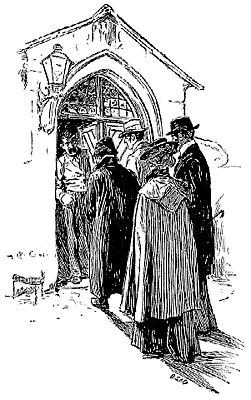
\includegraphics{images/sign410-sign-06.png}\end{center}

\noindent \begin{center}\noun{A short, deep-chested man stood in
the opening.}\end{center}
\end{figure}
There was a grumbling sound and a clanking and jarring of keys. The
door swung heavily back, and a short, deep-chested man stood in the
opening, with the yellow light of the lantern shining upon his protruded
face and twinkling distrustful eyes.

{}``That you, Mr.\ Thaddeus? But who are the others? I had no orders
about them from the master.''

{}``No, McMurdo? You surprise me! I told my brother last night that
I should bring some friends.''

{}``He ain't been out o' his room to-day, Mr.\ Thaddeus, and I have
no orders. You know very well that I must stick to regulations. I
can let you in, but your friends must just stop where they are.''

This was an unexpected obstacle. Thaddeus Sholto looked about him
in a perplexed and helpless manner. {}``This is too bad of you, McMurdo!''
he said. {}``If I guarantee them, that is enough for you. There is
the young lady, too. She cannot wait on the public road at this hour.''

{}``Very sorry, Mr.\ Thaddeus,'' said the porter, inexorably. {}``Folk
may be friends o' yours, and yet no friends o' the master's. He pays
me well to do my duty, and my duty I'll do. I don't know none o' your
friends.''

{}``Oh, yes you do, McMurdo,'' cried Sherlock Holmes, genially.
{}``I don't think you can have forgotten me. Don't you remember the
amateur who fought three rounds with you at Alison's rooms on the
night of your benefit four years back?''

{}``Not Mr.\ Sherlock Holmes!''\ roared the prize-fighter. {}``God's
truth!\ how could I have mistook you? If instead o' standin' there
so quiet you had just stepped up and given me that cross-hit of yours
under the jaw, I'd ha' known you without a question. Ah, you're one
that has wasted your gifts, you have! You might have aimed high, if
you had joined the fancy.''

{}``You see, Watson, if all else fails me I have still one of the
scientific professions open to me,'' said Holmes, laughing. {}``Our
friend won't keep us out in the cold now, I am sure.''

{}``In you come, sir, in you come,\mdsh{---}you and your friends,''
he answered. {}``Very sorry, Mr.\ Thaddeus, but orders are very
strict. Had to be certain of your friends before I let them in.''

Inside, a gravel path wound through desolate grounds to a huge clump
of a house, square and prosaic, all plunged in shadow save where a
moonbeam struck one corner and glimmered in a garret window. The vast
size of the building, with its gloom and its deathly silence, struck
a chill to the heart. Even Thaddeus Sholto seemed ill at ease, and
the lantern quivered and rattled in his hand.

{}``I cannot understand it,'' he said. {}``There must be some mistake.
I distinctly told Bartholomew that we should be here, and yet there
is no light in his window. I do not know what to make of it.''

{}``Does he always guard the premises in this way?'' asked Holmes.

{}``Yes; he has followed my father's custom. He was the favorite
son, you know, and I sometimes think that my father may have told
him more than he ever told me. That is Bartholomew's window up there
where the moonshine strikes. It is quite bright, but there is no light
from within, I think.''

{}``None,'' said Holmes. {}``But I see the glint of a light in
that little window beside the door.''

{}``Ah, that is the housekeeper's room. That is where old Mrs. Bernstone
sits. She can tell us all about it. But perhaps you would not mind
waiting here for a minute or two, for if we all go in together and
she has no word of our coming she may be alarmed. But hush! what is
that?''

He held up the lantern, and his hand shook until the circles of light
flickered and wavered all round us. Miss Morstan seized my wrist,
and we all stood with thumping hearts, straining our ears. From the
great black house there sounded through the silent night the saddest
and most pitiful of sounds,\mdsh{---}the shrill, broken whimpering
of a frightened woman.

{}``It is Mrs.\ Bernstone,'' said Sholto. {}``She is the only
woman in the house. Wait here. I shall be back in a moment.'' He
hurried for the door, and knocked in his peculiar way. We could see
a tall old woman admit him, and sway with pleasure at the very sight
of him.

{}``Oh, Mr.\ Thaddeus, sir, I am so glad you have come! I am so
glad you have come, Mr.\ Thaddeus, sir!'' We heard her reiterated
rejoicings until the door was closed and her voice died away into
a muffled monotone.

Our guide had left us the lantern. Holmes swung it slowly round, and
peered keenly at the house, and at the great rubbish-heaps which cumbered
the grounds. Miss Morstan and I stood together, and her hand was in
mine. A wondrous subtle thing is love, for here were we two who had
never seen each other before that day, between whom no word or even
look of affection had ever passed, and yet now in an hour of trouble
our hands instinctively sought for each other. I have marvelled at
it since, but at the time it seemed the most natural thing that I
should go out to her so, and, as she has often told me, there was
in her also the instinct to turn to me for comfort and protection.
So we stood hand in hand, like two children, and there was peace in
our hearts for all the dark things that surrounded us.

{}``What a strange place!''\ she said, looking round.

{}``It looks as though all the moles in England had been let loose
in it. I have seen something of the sort on the side of a hill near
Ballarat, where the prospectors had been at work.''

{}``And from the same cause,'' said Holmes. {}``These are the traces
of the treasure-seekers. You must remember that they were six years
looking for it. No wonder that the grounds look like a gravel-pit.''

At that moment the door of the house burst open, and Thaddeus Sholto
came running out, with his hands thrown forward and terror in his
eyes.

{}``There is something amiss with Bartholomew!''\ he cried. {}``I
am frightened! My nerves cannot stand it.'' He was, indeed, half
blubbering with fear, and his twitching feeble face peeping out from
the great Astrakhan collar had the helpless appealing expression of
a terrified child.

{}``Come into the house,'' said Holmes, in his crisp, firm way.

{}``Yes, do!'' pleaded Thaddeus Sholto. {}``I really do not feel
equal to giving directions.''

We all followed him into the housekeeper's room, which stood upon
the left-hand side of the passage. The old woman was pacing up and
down with a scared look and restless picking fingers, but the sight
of Miss Morstan appeared to have a soothing effect upon her.

{}``God bless your sweet calm face!''\ she cried, with an hysterical
sob. {}``It does me good to see you. Oh, but I have been sorely tried
this day!''

Our companion patted her thin, work-worn hand, and murmured some few
words of kindly womanly comfort which brought the color back into
the others bloodless cheeks.

{}``Master has locked himself in and will not answer me,'' she explained.
{}``All day I have waited to hear from him, for he often likes to
be alone; but an hour ago I feared that something was amiss, so I
went up and peeped through the key-hole. You must go up, Mr.\ Thaddeus,\mdsh{---}you
must go up and look for yourself. I have seen Mr.\ Bartholomew Sholto
in joy and in sorrow for ten long years, but I never saw him with
such a face on him as that.''

Sherlock Holmes took the lamp and led the way, for Thaddeus Sholto's
teeth were chattering in his head. So shaken was he that I had to
pass my hand under his arm as we went up the stairs, for his knees
were trembling under him. Twice as we ascended Holmes whipped his
lens out of his pocket and carefully examined marks which appeared
to me to be mere shapeless smudges of dust upon the cocoa-nut matting
which served as a stair-carpet. He walked slowly from step to step,
holding the lamp, and shooting keen glances to right and left. Miss
Morstan had remained behind with the frightened housekeeper.

The third flight of stairs ended in a straight passage of some length,
with a great picture in Indian tapestry upon the right of it and three
doors upon the left. Holmes advanced along it in the same slow and
methodical way, while we kept close at his heels, with our long black
shadows streaming backwards down the corridor. The third door was
that which we were seeking. Holmes knocked without receiving any answer,
and then tried to turn the handle and force it open. It was locked
on the inside, however, and by a broad and powerful bolt, as we could
see when we set our lamp up against it. The key being turned, however,
the hole was not entirely closed. Sherlock Holmes bent down to it,
and instantly rose again with a sharp intaking of the breath.

{}``There is something devilish in this, Watson,'' said he, more
moved than I had ever before seen him. {}``What do you make of it?''

I stooped to the hole, and recoiled in horror. Moonlight was streaming
into the room, and it was bright with a vague and shifty radiance.
Looking straight at me, and suspended, as it were, in the air, for
all beneath was in shadow, there hung a face,\mdsh{---}the very face
of our companion Thaddeus. There was the same high, shining head,
the same circular bristle of red hair, the same bloodless countenance.
The features were set, however, in a horrible smile, a fixed and unnatural
grin, which in that still and moonlit room was more jarring to the
nerves than any scowl or contortion. So like was the face to that
of our little friend that I looked round at him to make sure that
he was indeed with us. Then I recalled to mind that he had mentioned
to us that his brother and he were twins.

{}``This is terrible!'' I said to Holmes. {}``What is to be done?''

{}``The door must come down,'' he answered, and, springing against
it, he put all his weight upon the lock. It creaked and groaned, but
did not yield. Together we flung ourselves upon it once more, and
this time it gave way with a sudden snap, and we found ourselves within
Bartholomew Sholto's chamber.

It appeared to have been fitted up as a chemical laboratory. A double
line of glass-stoppered bottles was drawn up upon the wall opposite
the door, and the table was littered over with Bunsen burners, test-tubes,
and retorts. In the corners stood carboys of acid in wicker baskets.
One of these appeared to leak or to have been broken, for a stream
of dark-colored liquid had trickled out from it, and the air was heavy
with a peculiarly pungent, tar-like odor. A set of steps stood at
one side of the room, in the midst of a litter of lath and plaster,
and above them there was an opening in the ceiling large enough for
a man to pass through.\  at the foot of the steps a long coil of
rope was thrown carelessly together.

%
\begin{figure}[htbp]
\noindent \begin{center}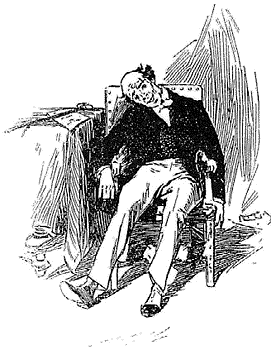
\includegraphics{images/sign410-sign-07.png}\end{center}

\noindent \begin{center}\noun{In a wooden arm-chair, the master
of the house was seated all in a heap, with his head sunk upon his
left shoulder, and that ghastly, inscrutable smile upon his face.}\end{center}
\end{figure}
By the table, in a wooden arm-chair, the master of the house was seated
all in a heap, with his head sunk upon his left shoulder, and that
ghastly, inscrutable smile upon his face. He was stiff and cold, and
had clearly been dead many hours. It seemed to me that not only his
features but all his limbs were twisted and turned in the most fantastic
fashion. By his hand upon the table there lay a peculiar instrument,\mdsh{---}a
brown, close-grained stick, with a stone head like a hammer, rudely
lashed on with coarse twine. Beside it was a torn sheet of note-paper
with some words scrawled upon it. Holmes glanced at it, and then handed
it to me.

{}``You see,'' he said, with a significant raising of the eyebrows.

In the light of the lantern I read, with a thrill of horror, {}``The
sign of the four.''

{}``In God's name, what does it all mean?'' I asked.

{}``It means murder,'' said he, stooping over the dead man. {}``Ah,
I expected it. Look here!'' He pointed to what looked like a long,
dark thorn stuck in the skin just above the ear.

{}``It looks like a thorn,'' said I.

{}``It is a thorn. You may pick it out. But be careful, for it is
poisoned.''

I took it up between my finger and thumb. It came away from the skin
so readily that hardly any mark was left behind. One tiny speck of
blood showed where the puncture had been.

{}``This is all an insoluble mystery to me,'' said I. {}``It grows
darker instead of clearer.''

{}``On the contrary,'' he answered, {}``it clears every instant.
I only require a few missing links to have an entirely connected case.''

We had almost forgotten our companion's presence since we entered
the chamber. He was still standing in the door-way, the very picture
of terror, wringing his hands and moaning to himself. Suddenly, however,
he broke out into a sharp, querulous cry.

{}``The treasure is gone!'' he said. {}``They have robbed him of
the treasure! There is the hole through which we lowered it. I helped
him to do it! I was the last person who saw him! I left him here last
night, and I heard him lock the door as I came down-stairs.''

{}``What time was that?''

{}``It was ten o'clock. And now he is dead, and the police will be
called in, and I shall be suspected of having had a hand in it. Oh,
yes, I am sure I shall. But you don't think so, gentlemen? Surely
you don't think that it was I? Is it likely that I would have brought
you here if it were I? Oh, dear!\ oh, dear! I know that I shall go
mad!'' He jerked his arms and stamped his feet in a kind of convulsive
frenzy.

{}``You have no reason for fear, Mr.\ Sholto,'' said Holmes, kindly,
putting his hand upon his shoulder. {}``Take my advice, and drive
down to the station to report this matter to the police. Offer to
assist them in every way. We shall wait here until your return.''

The little man obeyed in a half-stupefied fashion, and we heard him
stumbling down the stairs in the dark.


\chapter*{\raggedright Chapter VI. Sherlock Holmes Gives a Demonstration}

\addcontentsline{toc}{chapter}{Chapter VI. Sherlock Holmes Gives
a\\
Demonstration}

\markboth{The Sign of the Four}{Sherlock Holmes Gives a Demonstration}

{}``Now, Watson,'' said Holmes, rubbing his hands, {}``we have
half an hour to ourselves. Let us make good use of it. My case is,
as I have told you, almost complete; but we must not err on the side
of over-confidence. Simple as the case seems now, there may be something
deeper underlying it.''

{}``Simple!'' I ejaculated.

{}``Surely,'' said he, with something of the air of a clinical professor
expounding to his class. {}``Just sit in the corner there, that your
footprints may not complicate matters. Now to work! In the first place,
how did these folk come, and how did they go? The door has not been
opened since last night. How of the window?'' He carried the lamp
across to it, muttering his observations aloud the while, but addressing
them to himself rather than to me. {}``Window is snibbed on the inner
side. Framework is solid. No hinges at the side. Let us open it. No
water-pipe near. Roof quite out of reach. Yet a man has mounted by
the window. It rained a little last night. Here is the print of a
foot in mould upon the sill. And here is a circular muddy mark, and
here again upon the floor, and here again by the table. See here,
Watson! This is really a very pretty demonstration.''

I looked at the round, well-defined muddy discs. {}``This is not
a footmark,'' said I.

{}``It is something much more valuable to us. It is the impression
of a wooden stump. You see here on the sill is the boot-mark, a heavy
boot with the broad metal heel, and beside it is the mark of the timber-toe.''

{}``It is the wooden-legged man.''

{}``Quite so. But there has been some one else,\mdsh{---}a very
able and efficient ally. Could you scale that wall, doctor?''

I looked out of the open window. The moon still shone brightly on
that angle of the house. We were a good sixty feet from the ground,
and, look where I would, I could see no foothold, nor as much as a
crevice in the brick-work.

{}``It is absolutely impossible,'' I answered.

{}``Without aid it is so. But suppose you had a friend up here who
lowered you this good stout rope which I see in the corner, securing
one end of it to this great hook in the wall. Then, I think, if you
were an active man, you might swarm up, wooden leg and all. You would
depart, of course, in the same fashion, and your ally would draw up
the rope, untie it from the hook, shut the window, snib it on the
inside, and get away in the way that he originally came. As a minor
point it may be noted,'' he continued, fingering the rope, {}``that
our wooden-legged friend, though a fair climber, was not a professional
sailor. His hands were far from horny. My lens discloses more than
one blood-mark, especially towards the end of the rope, from which
I gather that he slipped down with such velocity that he took the
skin off his hand.''

{}``This is all very well,'' said I, {}``but the thing becomes
more unintelligible than ever. How about this mysterious ally? How
came he into the room?''

{}``Yes, the ally!''\ repeated Holmes, pensively. {}``There are
features of interest about this ally. He lifts the case from the regions
of the commonplace. I fancy that this ally breaks fresh ground in
the annals of crime in this country,\mdsh{---}though parallel cases
suggest themselves from India, and, if my memory serves me, from Senegambia.''

{}``How came he, then?''\ I reiterated. {}``The door is locked,
the window is inaccessible. Was it through the chimney?''

{}``The grate is much too small,'' he answered. {}``I had already
considered that possibility.''

{}``How then?''\ I persisted.

{}``You will not apply my precept,'' he said, shaking his head.
{}``How often have I said to you that when you have eliminated the
impossible whatever remains, \textit{however} \textit{improbable},
must be the truth? We know that he did not come through the door,
the window, or the chimney. We also know that he could not have been
concealed in the room, as there is no concealment possible. Whence,
then, did he come?''

{}``He came through the hole in the roof,'' I cried.

{}``Of course he did. He must have done so. If you will have the
kindness to hold the lamp for me, we shall now extend our researches
to the room above,\mdsh{---}the secret room in which the treasure
was found.''

He mounted the steps, and, seizing a rafter with either hand, he swung
himself up into the garret. Then, lying on his face, he reached down
for the lamp and held it while I followed him.

The chamber in which we found ourselves was about ten feet one way
and six the other. The floor was formed by the rafters, with thin
lath-and-plaster between, so that in walking one had to step from
beam to beam. The roof ran up to an apex, and was evidently the inner
shell of the true roof of the house. There was no furniture of any
sort, and the accumulated dust of years lay thick upon the floor.

{}``Here you are, you see,'' said Sherlock Holmes, putting his hand
against the sloping wall. {}``This is a trap-door which leads out
on to the roof. I can press it back, and here is the roof itself,
sloping at a gentle angle. This, then, is the way by which Number
One entered. Let us see if we can find one other traces of his individuality.''

%
\begin{figure}[htbp]
\noindent \begin{center}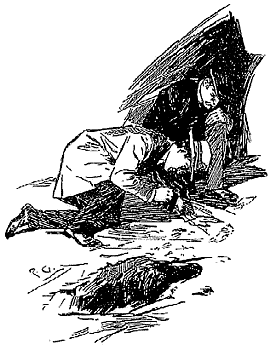
\includegraphics[%
  width=1\columnwidth]{images/sign410-sign-08.png}\end{center}

\noindent \begin{center}\noun{He held down the lamp to the floor.}\end{center}
\end{figure}
He held down the lamp to the floor, and as he did so I saw for the
second time that night a startled, surprised look come over his face.
For myself, as I followed his gaze my skin was cold under my clothes.
The floor was covered thickly with the prints of a naked foot,\mdsh{---}clear,
well defined, perfectly formed, but scarce half the size of those
of an ordinary man.

{}``Holmes,'' I said, in a whisper, {}``a child has done the horrid
thing.''

He had recovered his self-possession in an instant. {}``I was staggered
for the moment,'' he said, {}``but the thing is quite natural. My
memory failed me, or I should have been able to foretell it. There
is nothing more to be learned here. Let us go down.''

{}``What is your theory, then, as to those footmarks?''\ I asked,
eagerly, when we had regained the lower room once more.

{}``My dear Watson, try a little analysis yourself,'' said he, with
a touch of impatience. {}``You know my methods. Apply them, and it
will be instructive to compare results.''

{}``I cannot conceive anything which will cover the facts,'' I answered.

{}``It will be clear enough to you soon,'' he said, in an off-hand
way. {}``I think that there is nothing else of importance here, but
I will look.'' He whipped out his lens and a tape measure, and hurried
about the room on his knees, measuring, comparing, examining, with
his long thin nose only a few inches from the planks, and his beady
eyes gleaming and deep-set like those of a bird. So swift, silent,
and furtive were his movements, like those of a trained blood-hound
picking out a scent, that I could not but think what a terrible criminal
he would have made had he turned his energy and sagacity against the
law, instead of exerting them in its defense. As he hunted about,
he kept muttering to himself, and finally he broke out into a loud
crow of delight.

{}``We are certainly in luck,'' said he. {}``We ought to have very
little trouble now. Number One has had the misfortune to tread in
the creosote. You can see the outline of the edge of his small foot
here at the side of this evil-smelling mess. The carboy has been cracked,
You see, and the stuff has leaked out.''

{}``What then?'' I asked.

{}``Why, we have got him, that's all,'' said he. {}``I know a dog
that would follow that scent to the world's end. If a pack can track
a trailed herring across a shire, how far can a specially-trained
hound follow so pungent a smell as this? It sounds like a sum in the
rule of three. The answer should give us the\mdsh{---} But halloo!
here are the accredited representatives of the law.''

Heavy steps and the clamor of loud voices were audible from below,
and the hall door shut with a loud crash.

{}``Before they come,'' said Holmes, {}``just put your hand here
on this poor fellow's arm, and here on his leg. What do you feel?''

{}``The muscles are as hard as a board,'' I answered.

{}``Quite so. They are in a state of extreme contraction, far exceeding
the usual rigor mortis. Coupled with this distortion of the face,
this Hippocratic smile, or `\emph{risus sardonicus},' as the old writers
called it, what conclusion would it suggest to your mind?''

{}``Death from some powerful vegetable alkaloid,'' I answered,\mdsh{---}``some
strychnine-like substance which would produce tetanus.''

{}``That was the idea which occurred to me the instant I saw the
drawn muscles of the face. On getting into the room I at once looked
for the means by which the poison had entered the system. As you saw,
I discovered a thorn which had been driven or shot with no great force
into the scalp. You observe that the part struck was that which would
be turned towards the hole in the ceiling if the man were erect in
his chair. Now examine the thorn.''

I took it up gingerly and held it in the light of the lantern. It
was long, sharp, and black, with a glazed look near the point as though
some gummy substance had dried upon it. The blunt end had been trimmed
and rounded off with a knife.

{}``Is that an English thorn?'' he asked.

{}``No, it certainly is not.''

{}``With all these data you should be able to draw some just inference.
But here are the regulars: so the auxiliary forces may beat a retreat.''

As he spoke, the steps which had been coming nearer sounded loudly
on the passage, and a very stout, portly man in a gray suit strode
heavily into the room. He was red-faced, burly and plethoric, with
a pair of very small twinkling eyes which looked keenly out from between
swollen and puffy pouches. He was closely followed by an inspector
in uniform, and by the still palpitating Thaddeus Sholto.

{}``Here's a business!'' he cried, in a muffled, husky voice. {}``Here's
a pretty business! But who are all these? Why, the house seems to
be as full as a rabbit-warren!''

{}``I think you must recollect me, Mr.\ Athelney Jones,'' said
Holmes, quietly.

{}``Why, of course I do!''\ he wheezed. {}``It's Mr.\ Sherlock
Holmes, the theorist. Remember you! I'll never forget how you lectured
us all on causes and inferences and effects in the Bishopgate jewel
case. It's true you set us on the right track; but you'll own now
that it was more by good luck than good guidance.''

{}``It was a piece of very simple reasoning.''

{}``Oh, come, now, come! Never be ashamed to own up. But what is
all this? Bad business! Bad business! Stern facts here,\mdsh{---}no
room for theories. How lucky that I happened to be out at Norwood
over another case! I was at the station when the message arrived.
What d'you think the man died of?''

{}``Oh, this is hardly a case for me to theorize over,'' said Holmes,
dryly.

{}``No, no. Still, we can't deny that you hit the nail on the head
sometimes. Dear me! Door locked, I understand. Jewels worth half a
million missing. How was the window?''

{}``Fastened; but there are steps on the sill.''

{}``Well, well, if it was fastened the steps could have nothing to
do with the matter. That's common sense. Man might have died in a
fit; but then the jewels are missing. Ha! I have a theory. These flashes
come upon me at times.\mdsh{---} Just step outside, sergeant, and
you, Mr.\ Sholto. Your friend can remain.\mdsh{---} What do you
think of this, Holmes? Sholto was, on his own confession, with his
brother last night. The brother died in a fit, on which Sholto walked
off with the treasure. How's that?''

{}``On which the dead man very considerately got up and locked the
door on the inside.''

{}``Hum! There's a flaw there. Let us apply common sense to the matter.
This Thaddeus Sholto \textit{was} with his brother; there \textit{was}
a quarrel; so much we know. The brother is dead and the jewels are
gone. So much also we know. No one saw the brother from the time Thaddeus
left him. His bed had not been slept in. Thaddeus is evidently in
a most disturbed state of mind. His appearance is\mdsh{---}well,
not attractive. You see that I am weaving my web round Thaddeus. The
net begins to close upon him.''

{}``You are not quite in possession of the facts yet,'' said Holmes.
{}``This splinter of wood, which I have every reason to believe to
be poisoned, was in the man's scalp where you still see the mark;
this card, inscribed as you see it, was on the table; and beside it
lay this rather curious stone-headed instrument. How does all that
fit into your theory?''

{}``Confirms it in every respect,'' said the fat detective, pompously.
{}``House is full of Indian curiosities. Thaddeus brought this up,
and if this splinter be poisonous Thaddeus may as well have made murderous
use of it as any other man. The card is some hocus-pocus,\mdsh{---}a
blind, as like as not. The only question is, how did he depart? Ah,
of course, here is a hole in the roof.'' With great activity, considering
his bulk, he sprang up the steps and squeezed through into the garret,
and immediately afterwards we heard his exulting voice proclaiming
that he had found the trap-door.

{}``He can find something,'' remarked Holmes, shrugging his shoulders.
{}``He has occasional glimmerings of reason. \emph{Il n'y a pas des
sots si incommodes que ceux qui ont de l'esprit}!''

{}``You see!'' said Athelney Jones, reappearing down the steps again.
{}``Facts are better than mere theories, after all. My view of the
case is confirmed. There is a trap-door communicating with the roof,
and it is partly open.''

{}``It was I who opened it.''

{}``Oh, indeed! You did notice it, then?''\ He seemed a little
crestfallen at the discovery. {}``Well, whoever noticed it, it shows
how our gentleman got away. Inspector!''

{}``Yes, sir,'' from the passage.

%
\begin{figure}[htbp]
\noindent \begin{center}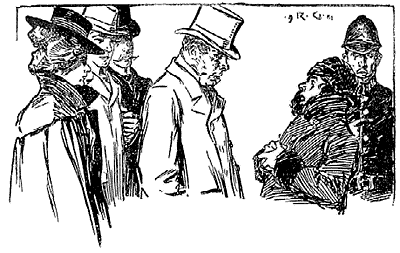
\includegraphics[%
  width=1\columnwidth]{images/sign410-sign-09.png}\end{center}

\noindent \begin{center}\noun{Mr.\ Sholto, it is my duty to inform
you that anything which you may say will be used against you.}\end{center}
\end{figure}
{}``Ask Mr.\ Sholto to step this way.\mdsh{---}Mr.\ Sholto, it
is my duty to inform you that anything which you may say will be used
against you. I arrest you in the queen's name as being concerned in
the death of your brother.''

{}``There, now! Didn't I tell you!''\ cried the poor little man,
throwing out his hands, and looking from one to the other of us.

{}``Don't trouble yourself about it, Mr.\ Sholto,'' said Holmes.
{}``I think that I can engage to clear you of the charge.''

{}``Don't promise too much, Mr.\ Theorist,\mdsh{---}don't promise
too much!'' snapped the detective. {}``You may find it a harder
matter than you think.''

{}``Not only will I clear him, Mr.\ Jones, but I will make you a
free present of the name and description of one of the two people
who were in this room last night. His name, I have every reason to
believe, is Jonathan Small. He is a poorly-educated man, small, active,
with his right leg off, and wearing a wooden stump which is worn away
upon the inner side. His left boot has a coarse, square-toed sole,
with an iron band round the heel. He is a middle-aged man, much sunburned,
and has been a convict. These few indications may be of some assistance
to you, coupled with the fact that there is a good deal of skin missing
from the palm of his hand. The other man\mdsh{---}''

{}``Ah!\ the other man\mdsh{---}?'' asked Athelney Jones, in a
sneering voice, but impressed none the less, as I could easily see,
by the precision of the other's manner.

{}``Is a rather curious person,'' said Sherlock Holmes, turning
upon his heel. {}``I hope before very long to be able to introduce
you to the pair of them.\mdsh{---} A word with you, Watson.''

He led me out to the head of the stair. {}``This unexpected occurrence,''
he said, {}``has caused us rather to lose sight of the original purpose
of our journey.''

{}``I have just been thinking so,'' I answered. {}``It is not right
that Miss Morstan should remain in this stricken house.''

{}``No. You must escort her home. She lives with Mrs.\ Cecil Forrester,
in Lower Camberwell: so it is not very far. I will wait for you here
if you will drive out again. Or perhaps you are too tired?''

{}``By no means. I don't think I could rest until I know more of
this fantastic business. I have seen something of the rough side of
life, but I give you my word that this quick succession of strange
surprises to-night has shaken my nerve completely. I should like,
however, to see the matter through with you, now that I have got so
far.''

{}``Your presence will be of great service to me,'' he answered.
{}``We shall work the case out independently, and leave this fellow
Jones to exult over any mare's-nest which he may choose to construct.
When you have dropped Miss Morstan I wish you to go on to No.\ 3
Pinchin Lane, down near the water's edge at Lambeth. The third house
on the right-hand side is a bird-stuffer's: Sherman is the name. You
will see a weasel holding a young rabbit in the window. Knock old
Sherman up, and tell him, with my compliments, that I want Toby at
once. You will bring Toby back in the cab with you.''

{}``A dog, I suppose.''

{}``Yes,\mdsh{---}a queer mongrel, with a most amazing power of
scent. I would rather have Toby's help than that of the whole detective
force of London.''

{}``I shall bring him, then,'' said I. {}``It is one now. I ought
to be back before three, if I can get a fresh horse.''

{}``And I,'' said Holmes, {}``shall see what I can learn from Mrs.
Bernstone, and from the Indian servant, who, Mr.\ Thaddeus tell me,
sleeps in the next garret. Then I shall study the great Jones's methods
and listen to his not too delicate sarcasms. `\emph{Wir sind gewohnt
das die Menschen verhoehnen was sie nicht verstehen}.' Goethe is always
pithy.''


\chapter*{\raggedright Chapter VII. The Episode of the Barrel}

\addcontentsline{toc}{chapter}{Chapter VII. The Episode of the Barrel}

\markboth{The Sign of the Four}{The Episode of the Barrel}

The police had brought a cab with them, and in this I escorted Miss
Morstan back to her home. After the angelic fashion of women, she
had borne trouble with a calm face as long as there was some one weaker
than herself to support, and I had found her bright and placid by
the side of the frightened housekeeper. In the cab, however, she first
turned faint, and then burst into a passion of weeping,\mdsh{---}so
sorely had she been tried by the adventures of the night. She has
told me since that she thought me cold and distant upon that journey.
She little guessed the struggle within my breast, or the effort of
self-restraint which held me back. My sympathies and my love went
out to her, even as my hand had in the garden. I felt that years of
the conventionalities of life could not teach me to know her sweet,
brave nature as had this one day of strange experiences. Yet there
were two thoughts which sealed the words of affection upon my lips.
She was weak and helpless, shaken in mind and nerve. It was to take
her at a disadvantage to obtrude love upon her at such a time. Worse
still, she was rich. If Holmes's researches were successful, she would
be an heiress. Was it fair, was it honorable, that a half-pay surgeon
should take such advantage of an intimacy which chance had brought
about? Might she not look upon me as a mere vulgar fortune-seeker?
I could not bear to risk that such a thought should cross her mind.
This Agra treasure intervened like an impassable barrier between us.

It was nearly two o'clock when we reached Mrs.\ Cecil Forrester's.
The servants had retired hours ago, but Mrs.\ Forrester had been
so interested by the strange message which Miss Morstan had received
that she had sat up in the hope of her return. She opened the door
herself, a middle-aged, graceful woman, and it gave me joy to see
how tenderly her arm stole round the other's waist and how motherly
was the voice in which she greeted her. She was clearly no mere paid
dependant, but an honored friend. I was introduced, and Mrs.\ Forrester
earnestly begged me to step in and tell her our adventures. I explained,
however, the importance of my errand, and promised faithfully to call
and report any progress which we might make with the case. As we drove
away I stole a glance back, and I still seem to see that little group
on the step, the two graceful, clinging figures, the half-opened door,
the hall light shining through stained glass, the barometer, and the
bright stair-rods. It was soothing to catch even that passing glimpse
of a tranquil English home in the midst of the wild, dark business
which had absorbed us.

And the more I thought of what had happened, the wilder and darker
it grew. I reviewed the whole extraordinary sequence of events as
I rattled on through the silent gas-lit streets. There was the original
problem: that at least was pretty clear now. The death of Captain
Morstan, the sending of the pearls, the advertisement, the letter,\mdsh{---}we
had had light upon all those events. They had only led us, however,
to a deeper and far more tragic mystery. The Indian treasure, the
curious plan found among Morstan's baggage, the strange scene at Major
Sholto's death, the rediscovery of the treasure immediately followed
by the murder of the discoverer, the very singular accompaniments
to the crime, the footsteps, the remarkable weapons, the words upon
the card, corresponding with those upon Captain Morstan's chart,\mdsh{---}here
was indeed a labyrinth in which a man less singularly endowed than
my fellow-lodger might well despair of ever finding the clue.

Pinchin Lane was a row of shabby two-storied brick houses in the lower
quarter of Lambeth. I had to knock for some time at No.\ 3 before
I could make my impression. At last, however, there was the glint
of a candle behind the blind, and a face looked out at the upper window.

{}``Go on, you drunken vagabone,'' said the face. {}``If you kick
up any more row I'll open the kennels and let out forty-three dogs
upon you.''

{}``If you'll let one out it's just what I have come for,'' said
I.

{}``Go on!''\ yelled the voice. {}``So help me gracious, I have
a wiper in the bag, an' I'll drop it on your 'ead if you don't hook
it.''

{}``But I want a dog,'' I cried.

{}``I won't be argued with!''\ shouted Mr.\ Sherman. {}``Now
stand clear, for when I say `three,' down goes the wiper.''

{}``Mr.\ Sherlock Holmes\mdsh{---}'' I began, but the words had
a most magical effect, for the window instantly slammed down, and
within a minute the door was unbarred and open. Mr.\ Sherman was
a lanky, lean old man, with stooping shoulders, a stringy neck, and
blue-tinted glasses.

%
\begin{figure}[htbp]
\noindent \begin{center}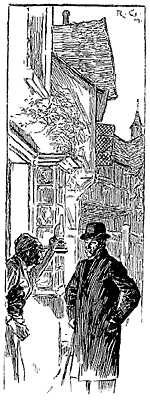
\includegraphics{images/sign410-sign-10.png}\end{center}

\noindent \begin{center}\noun{{}``A friend of Mr.\ Sherlock is
always welcome,'' said he.}\end{center}
\end{figure}
{}``A friend of Mr.\ Sherlock is always welcome,'' said he. {}``Step
in, sir. Keep clear of the badger; for he bites. Ah, naughty, naughty,
would you take a nip at the gentleman?'' This to a stoat which thrust
its wicked head and red eyes between the bars of its cage. {}``Don't
mind that, sir: it's only a slow-worm. It hain't got no fangs, so
I gives it the run o' the room, for it keeps the bettles down. You
must not mind my bein' just a little short wi' you at first, for I'm
guyed at by the children, and there's many a one just comes down this
lane to knock me up. What was it that Mr.\ Sherlock Holmes wanted,
sir?''

{}``He wanted a dog of yours.''

{}``Ah! that would be Toby.''

{}``Yes, Toby was the name.''

{}``Toby lives at No.\ 7 on the left here.'' He moved slowly forward
with his candle among the queer animal family which he had gathered
round him. In the uncertain, shadowy light I could see dimly that
there were glancing, glimmering eyes peeping down at us from every
cranny and corner. Even the rafters above our heads were lined by
solemn fowls, who lazily shifted their weight from one leg to the
other as our voices disturbed their slumbers.

Toby proved to an ugly, long-haired, lop-eared creature, half spaniel
and half lurcher, brown-and-white in color, with a very clumsy waddling
gait. It accepted after some hesitation a lump of sugar which the
old naturalist handed to me, and, having thus sealed an alliance,
it followed me to the cab, and made no difficulties about accompanying
me. It had just struck three on the Palace clock when I found myself
back once more at Pondicherry Lodge. The ex-prize-fighter McMurdo
had, I found, been arrested as an accessory, and both he and Mr.\ Sholto
had been marched off to the station. Two constables guarded the narrow
gate, but they allowed me to pass with the dog on my mentioning the
detective's name.

Holmes was standing on the door-step, with his hands in his pockets,
smoking his pipe.

{}``Ah, you have him there!''\ said he. {}``Good dog, then! Atheney
Jones has gone. We have had an immense display of energy since you
left. He has arrested not only friend Thaddeus, but the gatekeeper,
the housekeeper, and the Indian servant. We have the place to ourselves,
but for a sergeant up-stairs. Leave the dog here, and come up.''

We tied Toby to the hall table, and reascended the stairs. The room
was as he had left it, save that a sheet had been draped over the
central figure. A weary-looking police-sergeant reclined in the corner.

{}``Lend me your bull's-eye, sergeant,'' said my companion. {}``Now
tie this bit of card round my neck, so as to hang it in front of me.
Thank you. Now I must kick off my boots and stockings.\mdsh{---}
Just you carry them down with you, Watson. I am going to do a little
climbing. And dip my handkerchief into the creasote. That will do.
Now come up into the garret with me for a moment.''

We clambered up through the hole. Holmes turned his light once more
upon the footsteps in the dust.

{}``I wish you particularly to notice these footmarks,'' he said.
{}``Do you observe anything noteworthy about them?''

{}``They belong,'' I said, {}``to a child or a small woman.''

{}``Apart from their size, though. Is there nothing else?''

{}``They appear to be much as other footmarks.''

{}``Not at all. Look here! This is the print of a right foot in the
dust. Now I make one with my naked foot beside it. What is the chief
difference?''

{}``Your toes are all cramped together. The other print has each
toe distinctly divided.''

{}``Quite so. That is the point. Bear that in mind. Now, would you
kindly step over to that flap-window and smell the edge of the wood-work?
I shall stay here, as I have this handkerchief in my hand.''

I did as he directed, and was instantly conscious of a strong tarry
smell.

{}``That is where he put his foot in getting out. If \textit{you}
can trace him, I should think that Toby will have no difficulty. Now
run down-stairs, loose the dog, and look out for Blondin.''

By the time that I got out into the grounds Sherlock Holmes was on
the roof, and I could see him like an enormous glow-worm crawling
very slowly along the ridge. I lost sight of him behind a stack of
chimneys, but he presently reappeared, and then vanished once more
upon the opposite side. When I made my way round there I found him
seated at one of the corner eaves.

{}``That you, Watson?'' he cried.

{}``Yes.''

{}``This is the place. What is that black thing down there?''

{}``A water-barrel.''

{}``Top on it?''

{}``Yes.''

{}``No sign of a ladder?''

{}``No.''

{}``Confound the fellow! It's a most break-neck place. I ought to
be able to come down where he could climb up. The water-pipe feels
pretty firm. Here goes, anyhow.''

There was a scuffling of feet, and the lantern began to come steadily
down the side of the wall. Then with a light spring he came on to
the barrel, and from there to the earth.

{}``It was easy to follow him,'' he said, drawing on his stockings
and boots. {}``Tiles were loosened the whole way along, and in his
hurry he had dropped this. It confirms my diagnosis, as you doctors
express it.''

The object which he held up to me was a small pocket or pouch woven
out of colored grasses and with a few tawdry beads strung round it.
In shape and size it was not unlike a cigarette-case. Inside were
half a dozen spines of dark wood, sharp at one end and rounded at
the other, like that which had struck Bartholomew Sholto.

{}``They are hellish things,'' said he. {}``Look out that you don't
prick yourself. I'm delighted to have them, for the chances are that
they are all he has. There is the less fear of you or me finding one
in our skin before long. I would sooner face a Martini bullet, myself.
Are you game for a six-mile trudge, Watson?''

{}``Certainly,'' I answered.

{}``Your leg will stand it?''

{}``Oh, yes.''

{}``Here you are, doggy! Good old Toby! Smell it, Toby, smell it!''
He pushed the creasote handkerchief under the dog's nose, while the
creature stood with its fluffy legs separated, and with a most comical
cock to its head, like a connoisseur sniffing the bouquet of a famous
vintage. Holmes then threw the handkerchief to a distance, fastened
a stout cord to the mongrel's collar, and let him to the foot of the
water-barrel. The creature instantly broke into a succession of high,
tremulous yelps, and, with his nose on the ground, and his tail in
the air, pattered off upon the trail at a pace which strained his
leash and kept us at the top of our speed.

The east had been gradually whitening, and we could now see some distance
in the cold gray light. The square, massive house, with its black,
empty windows and high, bare walls, towered up, sad and forlorn, behind
us. Our course let right across the grounds, in and out among the
trenches and pits with which they were scarred and intersected. The
whole place, with its scattered dirt-heaps and ill-grown shrubs, had
a blighted, ill-omened look which harmonized with the black tragedy
which hung over it.

On reaching the boundary wall Toby ran along, whining eagerly, underneath
its shadow, and stopped finally in a corner screened by a young beech.
Where the two walls joined, several bricks had been loosened, and
the crevices left were worn down and rounded upon the lower side,
as though they had frequently been used as a ladder. Holmes clambered
up, and, taking the dog from me, he dropped it over upon the other
side.

{}``There's the print of wooden-leg's hand,'' he remarked, as I
mounted up beside him. {}``You see the slight smudge of blood upon
the white plaster. What a lucky thing it is that we have had no very
heavy rain since yesterday! The scent will lie upon the road in spite
of their eight-and-twenty hours' start.''

I confess that I had my doubts myself when I reflected upon the great
traffic which had passed along the London road in the interval. My
fears were soon appeased, however. Toby never hesitated or swerved,
but waddled on in his peculiar rolling fashion. Clearly, the pungent
smell of the creasote rose high above all other contending scents.

{}``Do not imagine,'' said Holmes, {}``that I depend for my success
in this case upon the mere chance of one of these fellows having put
his foot in the chemical. I have knowledge now which would enable
me to trace them in many different ways. This, however, is the readiest
and, since fortune has put it into our hands, I should be culpable
if I neglected it. It has, however, prevented the case from becoming
the pretty little intellectual problem which it at one time promised
to be. There might have been some credit to be gained out of it, but
for this too palpable clue.''

{}``There is credit, and to spare,'' said I. {}``I assure you,
Holmes, that I marvel at the means by which you obtain your results
in this case, even more than I did in the Jefferson Hope Murder. The
thing seems to me to be deeper and more inexplicable. How, for example,
could you describe with such confidence the wooden-legged man?''

{}``Pshaw, my dear boy! it was simplicity itself. I don't wish to
be theatrical. It is all patent and above-board. Two officers who
are in command of a convict-guard learn an important secret as to
buried treasure. A map is drawn for them by an Englishman named Jonathan
Small. You remember that we saw the name upon the chart in Captain
Morstan's possession. He had signed it in behalf of himself and his
associates,\mdsh{---}the sign of the four, as he somewhat dramatically
called it. Aided by this chart, the officers\mdsh{---}or one of them\mdsh{---}gets
the treasure and brings it to England, leaving, we will suppose, some
condition under which he received it unfulfilled. Now, then, why did
not Jonathan Small get the treasure himself? The answer is obvious.
The chart is dated at a time when Morstan was brought into close association
with convicts. Jonathan Small did not get the treasure because he
and his associates were themselves convicts and could not get away.''

{}``But that is mere speculation,'' said I.

{}``It is more than that. It is the only hypothesis which covers
the facts. Let us see how it fits in with the sequel. Major Sholto
remains at peace for some years, happy in the possession of his treasure.
Then he receives a letter from India which gives him a great fright.
What was that?''

{}``A letter to say that the men whom he had wronged had been set
free.''

{}``Or had escaped. That is much more likely, for he would have known
what their term of imprisonment was. It would not have been a surprise
to him. What does he do then? He guards himself against a wooden-legged
man,\mdsh{---}a white man, mark you, for he mistakes a white tradesman
for him, and actually fires a pistol at him. Now, only one white man's
name is on the chart. The others are Hindoos or Mohammedans. There
is no other white man. Therefore we may say with confidence that the
wooden-legged man is identical with Jonathan Small. Does the reasoning
strike you as being faulty?''

{}``No: it is clear and concise.''

{}``Well, now, let us put ourselves in the place of Jonathan Small.
Let us look at it from his point of view. He comes to England with
the double idea of regaining what he would consider to be his rights
and of having his revenge upon the man who had wronged him. He found
out where Sholto lived, and very possibly he established communications
with some one inside the house. There is this butler, Lal Rao, whom
we have not seen. Mrs.\ Bernstone gives him far from a good character.
Small could not find out, however, where the treasure was hid, for
no one ever knew, save the major and one faithful servant who had
died. Suddenly Small learns that the major is on his death-bed. In
a frenzy lest the secret of the treasure die with him, he runs the
gauntlet of the guards, makes his way to the dying man's window, and
is only deterred from entering by the presence of his two sons. Mad
with hate, however, against the dead man, he enters the room that
night, searches his private papers in the hope of discovering some
memorandum relating to the treasure, and finally leaves a memento
of his visit in the short inscription upon the card. He had doubtless
planned beforehand that should he slay the major he would leave some
such record upon the body as a sign that it was not a common murder,
but, from the point of view of the four associates, something in the
nature of an act of justice. Whimsical and bizarre conceits of this
kind are common enough in the annals of crime, and usually afford
valuable indications as to the criminal. Do you follow all this?''

{}``Very clearly.''

{}``Now, what could Jonathan Small do? He could only continue to
keep a secret watch upon the efforts made to find the treasure. Possibly
he leaves England and only comes back at intervals. Then comes the
discovery of the garret, and he is instantly informed of it. We again
trace the presence of some confederate in the household. Jonathan,
with his wooden leg, is utterly unable to reach the lofty room of
Bartholomew Sholto. He takes with him, however, a rather curious associate,
who gets over this difficulty, but dips his naked foot into creasote,
whence come Toby, and a six-mile limp for a half-pay officer with
a damaged \emph{tendo Achillis}.''

{}``But it was the associate, and not Jonathan, who committed the
crime.''

{}``Quite so. And rather to Jonathan's disgust, to judge by the way
the stamped about when he got into the room. He bore no grudge against
Bartholomew Sholto, and would have preferred if he could have been
simply bound and gagged. He did not wish to put his head in a halter.
There was no help for it, however: the savage instincts of his companion
had broken out, and the poison had done its work: so Jonathan Small
left his record, lowered the treasure-box to the ground, and followed
it himself. That was the train of events as far as I can decipher
them. Of course as to his personal appearance he must be middle-aged,
and must be sunburned after serving his time in such an oven as the
Andamans. His height is readily calculated from the length of his
stride, and we know that he was bearded. His hairiness was the one
point which impressed itself upon Thaddeus Sholto when he saw him
at the window. I don't know that there is anything else.''

{}``The associate?''

{}``Ah, well, there is no great mystery in that. But you will know
all about it soon enough. How sweet the morning air is! See how that
one little cloud floats like a pink feather from some gigantic flamingo.
Now the red rim of the sun pushes itself over the London cloud-bank.
It shines on a good many folk, but on none, I dare bet, who are on
a stranger errand than you and I.\  How small we feel with our petty
ambitions and strivings in the presence of the great elemental forces
of nature! Are you well up in your Jean Paul?''

{}``Fairly so. I worked back to him through Carlyle.''

{}``That was like following the brook to the parent lake. He makes
one curious but profound remark. It is that the chief proof of man's
real greatness lies in his perception of his own smallness. It argues,
you see, a power of comparison and of appreciation which is in itself
a proof of nobility. There is much food for thought in Richter. You
have not a pistol, have you?''

{}``I have my stick.''

{}``It is just possible that we may need something of the sort if
we get to their lair. Jonathan I shall leave to you, but if the other
turns nasty I shall shoot him dead.'' He took out his revolver as
he spoke, and, having loaded two of the chambers, he put it back into
the right-hand pocket of his jacket.

%
\begin{figure}[htbp]
\noindent \begin{center}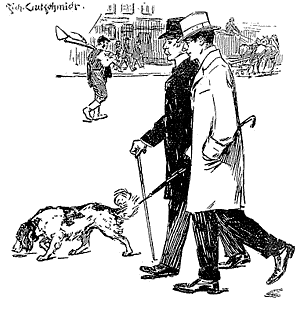
\includegraphics[%
  width=1\columnwidth]{images/sign410-sign-11.png}\end{center}

\noindent \begin{center}\noun{We had during this time been following
the guidance of Toby.}\end{center}
\end{figure}
We had during this time been following the guidance of Toby down the
half-rural villa-lined roads which lead to the metropolis. Now, however,
we were beginning to come among continuous streets, where laborers
and dockmen were already astir, and slatternly women were taking down
shutters and brushing door-steps. At the square-topped corner public
houses business was just beginning, and rough-looking men were emerging,
rubbing their sleeves across their beards after their morning wet.
Strange dogs sauntered up and stared wonderingly at us as we passed,
but our inimitable Toby looked neither to the right nor to the left,
but trotted onwards with his nose to the ground and an occasional
eager whine which spoke of a hot scent.

We had traversed Streatham, Brixton, Camberwell, and now found ourselves
in Kennington Lane, having borne away through the side-streets to
the east of the Oval. The men whom we pursued seemed to have taken
a curiously zigzag road, with the idea probably of escaping observation.
They had never kept to the main road if a parallel side-street would
serve their turn. At the foot of Kennington Lane they had edged away
to the left through Bond Street and Miles Street. Where the latter
street turns into Knight's Place, Toby ceased to advance, but began
to run backwards and forwards with one ear cocked and the other drooping,
the very picture of canine indecision. Then he waddled round in circles,
looking up to us from time to time, as if to ask for sympathy in his
embarrassment.

{}``What the deuce is the matter with the dog?''\ growled Holmes.
{}``They surely would not take a cab, or go off in a balloon.''

{}``Perhaps they stood here for some time,'' I suggested.

{}``Ah! it's all right. He's off again,'' said my companion, in
a tone of relief.

He was indeed off, for after sniffing round again he suddenly made
up his mind, and darted away with an energy and determination such
as he had not yet shown. The scent appeared to be much hotter than
before, for he had not even to put his nose on the ground, but tugged
at his leash and tried to break into a run. I cold see by the gleam
in Holmes's eyes that he thought we were nearing the end of our journey.

Our course now ran down Nine Elms until we came to Broderick and Nelson's
large timber-yard, just past the White Eagle tavern. Here the dog,
frantic with excitement, turned down through the side-gate into the
enclosure, where the sawyers were already at work. On the dog raced
through sawdust and shavings, down an alley, round a passage, between
two wood-piles, and finally, with a triumphant yelp, sprang upon a
large barrel which still stood upon the hand-trolley on which it had
been brought. With lolling tongue and blinking eyes, Toby stood upon
the cask, looking from one to the other of us for some sign of appreciation.
The staves of the barrel and the wheels of the trolley were smeared
with a dark liquid, and the whole air was heavy with the smell of
creasote.

Sherlock Holmes and I looked blankly at each other, and then burst
simultaneously into an uncontrollable fit of laughter.


\chapter*{\raggedright Chapter VIII. The Baker Street Irregulars}

\addcontentsline{toc}{chapter}{Chapter VIII. The Baker Street Irregulars}

\markboth{The Sign of the Four}{The Baker Street Irregulars}

{}``What now?'' I asked. {}``Toby has lost his character for infallibility.''

{}``He acted according to his lights,'' said Holmes, lifting him
down from the barrel and walking him out of the timber-yard. {}``If
you consider how much creasote is carted about London in one day,
it is no great wonder that our trail should have been crossed. It
is much used now, especially for the seasoning of wood. Poor Toby
is not to blame.''

{}``We must get on the main scent again, I suppose.''

{}``Yes. And, fortunately, we have no distance to go. Evidently what
puzzled the dog at the corner of Knight's Place was that there were
two different trails running in opposite directions. We took the wrong
one. It only remains to follow the other.''

There was no difficulty about this. On leading Toby to the place where
he had committed his fault, he cast about in a wide circle and finally
dashed off in a fresh direction.

{}``We must take care that he does not now bring us to the place
where the creasote-barrel came from,'' I observed.

{}``I had thought of that. But you notice that he keeps on the pavement,
whereas the barrel passed down the roadway. No, we are on the true
scent now.''

It tended down towards the river-side, running through Belmont Place
and Prince's Street. At the end of Broad Street it ran right down
to the water's edge, where there was a small wooden wharf. Toby led
us to the very edge of this, and there stood whining, looking out
on the dark current beyond.

{}``We are out of luck,'' said Holmes. {}``They have taken to a
boat here.'' Several small punts and skiffs were lying about in the
water and on the edge of the wharf. We took Toby round to each in
turn, but, though he sniffed earnestly, he made no sign.

Close to the rude landing-stage was a small brick house, with a wooden
placard slung out through the second window. {}``Mordecai Smith''
was printed across it in large letters, and, underneath, {}``Boats
to hire by the hour or day.'' A second inscription above the door
informed us that a steam launch was kept,\mdsh{---}a statement which
was confirmed by a great pile of coke upon the jetty. Sherlock Holmes
looked slowly round, and his face assumed an ominous expression.

{}``This looks bad,'' said he. {}``These fellows are sharper than
I expected. They seem to have covered their tracks. There has, I fear,
been preconcerted management here.''

He was approaching the door of the house, when it opened, and a little,
curly-headed lad of six came running out, followed by a stoutish,
red-faced woman with a large sponge in her hand.

{}``You come back and be washed, Jack,'' she shouted. {}``Come
back, you young imp; for if your father comes home and finds you like
that, he'll let us hear of it.''

%
\begin{figure}[htbp]
\noindent \begin{center}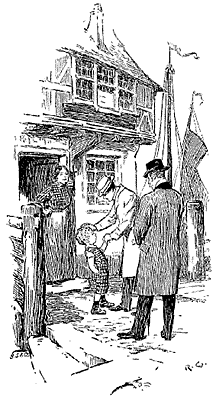
\includegraphics{images/sign410-sign-12.png}\end{center}

\noindent \begin{center}\noun{{}``Dear little chap!''\ said Holmes,
strategically.}\end{center}
\end{figure}
{}``Dear little chap!''\ said Holmes, strategically. {}``What
a rosy-cheeked young rascal! Now, Jack, is there anything you would
like?''

The youth pondered for a moment. {}``I'd like a shillin','' said
he.

{}``Nothing you would like better?''

{}``I'd like two shillin' better,'' the prodigy answered, after
some thought.

{}``Here you are, then! Catch!\mdsh{---}A fine child, Mrs.\ Smith!''

{}``Lor' bless you, sir, he is that, and forward. He gets a'most
too much for me to manage, 'specially when my man is away days at
a time.''

{}``Away, is he?''\ said Holmes, in a disappointed voice. {}``I
am sorry for that, for I wanted to speak to Mr.\ Smith.''

{}``He's been away since yesterday mornin', sir, and, truth to tell,
I am beginnin' to feel frightened about him. But if it was about a
boat, sir, maybe I could serve as well.''

{}``I wanted to hire his steam launch.''

{}``Why, bless you, sir, it is in the steam launch that he has gone.
That's what puzzles me; for I know there ain't more coals in her than
would take her to about Woolwich and back. If he'd been away in the
barge I'd ha' thought nothin'; for many a time a job has taken him
as far as Gravesend, and then if there was much doin' there he might
ha' stayed over. But what good is a steam launch without coals?''

{}``He might have bought some at a wharf down the river.''

{}``He might, sir, but it weren't his way. Many a time I've heard
him call out at the prices they charge for a few odd bags. Besides,
I don't like that wooden-legged man, wi' his ugly face and outlandish
talk. What did he want always knockin' about here for?''

{}``A wooden-legged man?''\ said Holmes, with bland surprise.

{}``Yes, sir, a brown, monkey-faced chap that's called more'n once
for my old man. It was him that roused him up yesternight, and, what's
more, my man knew he was comin', for he had steam up in the launch.
I tell you straight, sir, I don't feel easy in my mind about it.''

{}``But, my dear Mrs.\ Smith,'' said Holmes, shrugging his shoulders,
{}``You are frightening yourself about nothing. How could you possibly
tell that it was the wooden-legged man who came in the night? I don't
quite understand how you can be so sure.''

{}``His voice, sir. I knew his voice, which is kind o' thick and
foggy. He tapped at the winder,\mdsh{---}about three it would be.
`Show a leg, matey,' says he: `time to turn out guard.' My old man
woke up Jim,\mdsh{---}that's my eldest,\mdsh{---}and away they went,
without so much as a word to me. I could hear the wooden leg clackin'
on the stones.''

{}``And was this wooden-legged man alone?''

{}``Couldn't say, I am sure, sir. I didn't hear no one else.''

{}``I am sorry, Mrs.\ Smith, for I wanted a steam launch, and I
have heard good reports of the\mdsh{---} Let me see, what is her
name?''

{}``The \emph{Aurora}, sir.''

{}``Ah! She's not that old green launch with a yellow line, very
broad in the beam?''

{}``No, indeed. She's as trim a little thing as any on the river.
She's been fresh painted, black with two red streaks.''

{}``Thanks. I hope that you will hear soon from Mr.\ Smith. I am
going down the river; and if I should see anything of the \emph{Aurora}
I shall let him know that you are uneasy. A black funnel, you say?''

{}``No, sir. Black with a white band.''

{}``Ah, of course. It was the sides which were black. Good-morning,
Mrs.\ Smith.\mdsh{---} There is a boatman here with a wherry, Watson.
We shall take it and cross the river.

{}``The main thing with people of that sort,'' said Holmes, as we
sat in the sheets of the wherry, {}``is never to let them think that
their information can be of the slightest importance to you. If you
do, they will instantly shut up like an oyster. If you listen to them
under protest, as it were, you are very likely to get what you want.''

{}``Our course now seems pretty clear,'' said I.

{}``What would you do, then?''

{}``I would engage a launch and go down the river on the track of
the \emph{Aurora}.''

{}``My dear fellow, it would be a colossal task. She may have touched
at any wharf on either side of the stream between here and Greenwich.
Below the bridge there is a perfect labyrinth of landing-places for
miles. It would take you days and days to exhaust them, if you set
about it alone.''

{}``Employ the police, then.''

{}``No. I shall probably call Athelney Jones in at the last moment.
He is not a bad fellow, and I should not like to do anything which
would injure him professionally. But I have a fancy for working it
out myself, now that we have gone so far.''

{}``Could we advertise, then, asking for information from wharfingers?''

{}``Worse and worse! Our men would know that the chase was hot at
their heels, and they would be off out of the country. As it is, they
are likely enough to leave, but as long as they think they are perfectly
safe they will be in no hurry. Jones's energy will be of use to us
there, for his view of the case is sure to push itself into the daily
press, and the runaways will think that every one is off on the wrong
scent.''

{}``What are we to do, then?'' I asked, as we landed near Millbank
Penitentiary.

{}``Take this hansom, drive home, have some breakfast, and get an
hour's sleep. It is quite on the cards that we may be afoot to-night
again. Stop at a telegraph-office, cabby! We will keep Toby, for he
may be of use to us yet.''

We pulled up at the Great Peter Street post-office, and Holmes despatched
his wire. {}``Whom do you think that is to?'' he asked, as we resumed
our journey.

{}``I am sure I don't know.''

{}``You remember the Baker Street division of the detective police
force whom I employed in the Jefferson Hope case?''

{}``Well,'' said I, laughing.

{}``This is just the case where they might be invaluable. If they
fail, I have other resources; but I shall try them first. That wire
was to my dirty little lieutenant, Wiggins, and I expect that he and
his gang will be with us before we have finished our breakfast.''

It was between eight and nine o'clock now, and I was conscious of
a strong reaction after the successive excitements of the night. I
was limp and weary, befogged in mind and fatigued in body. I had not
the professional enthusiasm which carried my companion on, nor could
I look at the matter as a mere abstract intellectual problem. As far
as the death of Bartholomew Sholto went, I had heard little good of
him, and could feel no intense antipathy to his murderers. The treasure,
however, was a different matter. That, or part of it, belonged rightfully
to Miss Morstan. While there was a chance of recovering it I was ready
to devote my life to the one object. True, if I found it it would
probably put her forever beyond my reach. Yet it would be a petty
and selfish love which would be influenced by such a thought as that.
If Holmes could work to find the criminals, I had a tenfold stronger
reason to urge me on to find the treasure.

A bath at Baker Street and a complete change freshened me up wonderfully.
When I came down to our room I found the breakfast laid and Homes
pouring out the coffee.

{}``Here it is,'' said he, laughing, and pointing to an open newspaper.
{}``The energetic Jones and the ubiquitous reporter have fixed it
up between them. But you have had enough of the case. Better have
your ham and eggs first.''

I took the paper from him and read the short notice, which was headed
{}``Mysterious Business at Upper Norwood.''

\begin{quote}

``About twelve o'clock last night,'' said the \textit{Standard}, ``Mr.\ Bartholomew Sholto, of Pondicherry Lodge, Upper Norwood, was found dead in his room under circumstances which point to foul play. As far as we can learn, no actual traces of violence were found upon Mr.\ Sholto's person, but a valuable collection of Indian gems which the deceased gentleman had inherited from his father has been carried off. The discovery was first made by Mr.\ Sherlock Holmes and Dr.\ Watson, who had called at the house with Mr.\ Thaddeus Sholto, brother of the deceased. By a singular piece of good fortune, Mr.\ Athelney Jones, the well-known member of the detective police force, happened to be at the Norwood Police Station, and was on the ground within half an hour of the first alarm. His trained and experienced faculties were at once directed towards the detection of the criminals, with the gratifying result that the brother, Thaddeus Sholto, has already been arrested, together with the housekeeper, Mrs.\ Bernstone, an Indian butler named Lal Rao, and a porter, or gatekeeper, named McMurdo. It is quite certain that the thief or thieves were well acquainted with the house, for Mr.\ Jones's well-known technical knowledge and his powers of minute observation have enabled him to prove conclusively that the miscreants could not have entered by the door or by the window, but must have made their way across the roof of the building, and so through a trap-door into a room which communicated with that in which the body was found. This fact, which has been very clearly made out, proves conclusively that it was no mere haphazard burglary. The prompt and energetic action of the officers of the law shows the great advantage of the presence on such occasions of a single vigorous and masterful mind. We cannot but think that it supplies an argument to those who would wish to see our detectives more decentralized, and so brought into closer and more effective touch with the cases which it is their duty to investigate.''

\end{quote}

{}``Isn't it gorgeous!'' said Holmes, grinning over his coffee-cup.
{}``What do you think of it?''

{}``I think that we have had a close shave ourselves of being arrested
for the crime.''

{}``So do I.\  I wouldn't answer for our safety now, if he should
happen to have another of his attacks of energy.''

At this moment there was a loud ring at the bell, and I could hear
Mrs.\ Hudson, our landlady, raising her voice in a wail of expostulation
and dismay.

{}``By heaven, Holmes,'' I said, half rising, {}``I believe that
they are really after us.''

{}``No, it's not quite so bad as that. It is the unofficial force,\mdsh{---}the
Baker Street irregulars.''

As he spoke, there came a swift pattering of naked feet upon the stairs,
a clatter of high voices, and in rushed a dozen dirty and ragged little
street-Arabs. There was some show of discipline among them, despite
their tumultuous entry, for they instantly drew up in line and stood
facing us with expectant faces. One of their number, taller and older
than the others, stood forward with an air of lounging superiority
which was very funny in such a disreputable little scarecrow.

{}``Got your message, sir,'' said he, {}``and brought 'em on sharp.
Three bob and a tanner for tickets.''

{}``Here you are,'' said Holmes, producing some silver. {}``In
future they can report to you, Wiggins, and you to me. I cannot have
the house invaded in this way. However, it is just as well that you
should all hear the instructions. I want to find the whereabouts of
a steam launch called the \emph{Aurora}, owner Mordecai Smith, black
with two red streaks, funnel black with a white band. She is down
the river somewhere. I want one boy to be at Mordecai Smith's landing-stage
opposite Millbank to say if the boat comes back. You must divide it
out among yourselves, and do both banks thoroughly. Let me know the
moment you have news. Is that all clear?''

{}``Yes, guv'nor,'' said Wiggins.

%
\begin{figure}[htbp]
\noindent \begin{center}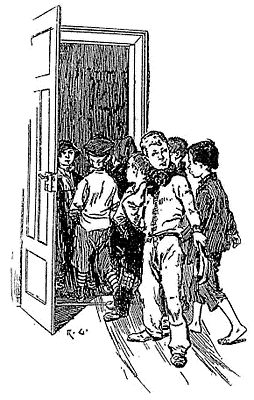
\includegraphics{images/sign410-sign-13.png}\end{center}

\noindent \begin{center}\noun{And away they buzzed down the stairs.}\end{center}
\end{figure}
{}``The old scale of pay, and a guinea to the boy who finds the boat.
Here's a day in advance. Now off you go!'' He handed them a shilling
each, and away they buzzed down the stairs, and I saw them a moment
later streaming down the street.

{}``If the launch is above water they will find her,'' said Holmes,
as he rose from the table and lit his pipe. {}``They can go everywhere,
see everything, overhear every one. I expect to hear before evening
that they have spotted her. In the mean while, we can do nothing but
await results. We cannot pick up the broken trail until we find either
the \emph{Aurora} or Mr.\ Mordecai Smith.''

{}``Toby could eat these scraps, I dare say. Are you going to bed,
Holmes?''

{}``No: I am not tired. I have a curious constitution. I never remember
feeling tired by work, though idleness exhausts me completely. I am
going to smoke and to think over this queer business to which my fair
client has introduced us. If ever man had an easy task, this of ours
ought to be. Wooden-legged men are not so common, but the other man
must, I should think, be absolutely unique.''

{}``That other man again!''

{}``I have no wish to make a mystery of him,\mdsh{---}to you, anyway.
But you must have formed your own opinion. Now, do consider the data.
Diminutive footmarks, toes never fettered by boots, naked feet, stone-headed
wooden mace, great agility, small poisoned darts. What do you make
of all this?''

{}``A savage!''\ I exclaimed. {}``Perhaps one of those Indians
who were the associates of Jonathan Small.''

{}``Hardly that,'' said he. {}``When first I saw signs of strange
weapons I was inclined to think so; but the remarkable character of
the footmarks caused me to reconsider my views. Some of the inhabitants
of the Indian Peninsula are small men, but none could have left such
marks as that. The Hindoo proper has long and thin feet. The sandal-wearing
Mohammedan has the great toe well separated from the others, because
the thong is commonly passed between. These little darts, too, could
only be shot in one way. They are from a blow-pipe. Now, then, where
are we to find our savage?''

{}``South American,'' I hazarded.

He stretched his hand up, and took down a bulky volume from the shelf.
{}``This is the first volume of a gazetteer which is now being published.
It may be looked upon as the very latest authority. What have we here?
`Andaman Islands, situated 340 miles to the north of Sumatra, in the
Bay of Bengal.' Hum!\ hum! What's all this? Moist climate, coral
reefs, sharks, Port Blair, convict-barracks, Rutland Island, cottonwoods\mdsh{---}
Ah, here we are. `The aborigines of the Andaman Islands may perhaps
claim the distinction of being the smallest race upon this earth,
though some anthropologists prefer the Bushmen of Africa, the Digger
Indians of America, and the Terra del Fuegians. The average height
is rather below four feet, although many full-grown adults may be
found who are very much smaller than this. They are a fierce, morose,
and intractable people, though capable of forming most devoted friendships
when their confidence has once been gained.' Mark that, Watson. Now,
then, listen to this. `They are naturally hideous, having large, misshapen
heads, small, fierce eyes, and distorted features. Their feet and
hands, however, are remarkably small. So intractable and fierce are
they that all the efforts of the British official have failed to win
them over in any degree. They have always been a terror to shipwrecked
crews, braining the survivors with their stone-headed clubs, or shooting
them with their poisoned arrows. These massacres are invariably concluded
by a cannibal feast.' Nice, amiable people, Watson! If this fellow
had been left to his own unaided devices this affair might have taken
an even more ghastly turn. I fancy that, even as it is, Jonathan Small
would give a good deal not to have employed him.''

{}``But how came he to have so singular a companion?''

{}``Ah, that is more than I can tell. Since, however, we had already
determined that Small had come from the Andamans, it is not so very
wonderful that this islander should be with him. No doubt we shall
know all about it in time. Look here, Watson; you look regularly done.
Lie down there on the sofa, and see if I can put you to sleep.''

He took up his violin from the corner, and as I stretched myself out
he began to play some low, dreamy, melodious air,\mdsh{---}his own,
no doubt, for he had a remarkable gift for improvisation. I have a
vague remembrance of his gaunt limbs, his earnest face, and the rise
and fall of his bow. Then I seemed to be floated peacefully away upon
a soft sea of sound, until I found myself in dream-land, with the
sweet face of Mary Morstan looking down upon me.


\chapter*{\raggedright Chapter IX. A Break in the Chain}

\addcontentsline{toc}{chapter}{Chapter IX. A Break in the Chain}

\markboth{The Sign of the Four}{A Break in the Chain}

It was late in the afternoon before I woke, strengthened and refreshed.
Sherlock Holmes still sat exactly as I had left him, save that he
had laid aside his violin and was deep in a book. He looked across
at me, as I stirred, and I noticed that his face was dark and troubled.

{}``You have slept soundly,'' he said. {}``I feared that our talk
would wake you.''

{}``I heard nothing,'' I answered. {}``Have you had fresh news,
then?''

{}``Unfortunately, no. I confess that I am surprised and disappointed.
I expected something definite by this time. Wiggins has just been
up to report. He says that no trace can be found of the launch. It
is a provoking check, for every hour is of importance.''

{}``Can I do anything? I am perfectly fresh now, and quite ready
for another night's outing.''

{}``No, we can do nothing. We can only wait. If we go ourselves,
the message might come in our absence, and delay be caused. You can
do what you will, but I must remain on guard.''

{}``Then I shall run over to Camberwell and call upon Mrs.\ Cecil
Forrester. She asked me to, yesterday.''

{}``On Mrs.\ Cecil Forrester?''\ asked Holmes, with the twinkle
of a smile in his eyes.

{}``Well, of course Miss Morstan too. They were anxious to hear what
happened.''

{}``I would not tell them too much,'' said Holmes. {}``Women are
never to be entirely trusted,\mdsh{---}not the best of them.''

I did not pause to argue over this atrocious sentiment. {}``I shall
be back in an hour or two,'' I remarked.

{}``All right! Good luck! But, I say, if you are crossing the river
you may as well return Toby, for I don't think it is at all likely
that we shall have any use for him now.''

I took our mongrel accordingly, and left him, together with a half-sovereign,
at the old naturalist's in Pinchin Lane. At Camberwell I found Miss
Morstan a little weary after her night's adventures, but very eager
to hear the news. Mrs.\ Forrester, too, was full of curiosity. I
told them all that we had done, suppressing, however, the more dreadful
parts of the tragedy. Thus, although I spoke of Mr.\ Sholto's death,
I said nothing of the exact manner and method of it. With all my omissions,
however, there was enough to startle and amaze them.

{}``It is a romance!'' cried Mrs.\ Forrester. {}``An injured lady,
half a million in treasure, a black cannibal, and a wooden-legged
ruffian. They take the place of the conventional dragon or wicked
earl.''

{}``And two knight-errants to the rescue,'' added Miss Morstan,
with a bright glance at me.

{}``Why, Mary, your fortune depends upon the issue of this search.
I don't think that you are nearly excited enough. Just imagine what
it must be to be so rich, and to have the world at your feet!''

It sent a little thrill of joy to my heart to notice that she showed
no sign of elation at the prospect. On the contrary, she gave a toss
of her proud head, as though the matter were one in which she took
small interest.

{}``It is for Mr.\ Thaddeus Sholto that I am anxious,'' she said.
{}``Nothing else is of any consequence; but I think that he has behaved
most kindly and honorably throughout. It is our duty to clear him
of this dreadful and unfounded charge.''

It was evening before I left Camberwell, and quite dark by the time
I reached home. My companion's book and pipe lay by his chair, but
he had disappeared. I looked about in the hope of seeing a note, but
there was none.

{}``I suppose that Mr.\ Sherlock Holmes has gone out,'' I said
to Mrs. Hudson as she came up to lower the blinds.

{}``No, sir. He has gone to his room, sir. Do you know, sir,'' sinking
her voice into an impressive whisper, {}``I am afraid for his health?''

{}``Why so, Mrs.\ Hudson?''

{}``Well, he's that strange, sir. After you was gone he walked and
he walked, up and down, and up and down, until I was weary of the
sound of his footstep. Then I heard him talking to himself and muttering,
and every time the bell rang out he came on the stairhead, with `What
is that, Mrs.\ Hudson?' And now he has slammed off to his room, but
I can hear him walking away the same as ever. I hope he's not going
to be ill, sir. I ventured to say something to him about cooling medicine,
but he turned on me, sir, with such a look that I don't know how ever
I got out of the room.''

{}``I don't think that you have any cause to be uneasy, Mrs. Hudson,''
I answered. {}``I have seen him like this before. He has some small
matter upon his mind which makes him restless.'' I tried to speak
lightly to our worthy landlady, but I was myself somewhat uneasy when
through the long night I still from time to time heard the dull sound
of his tread, and knew how his keen spirit was chafing against this
involuntary inaction.

At breakfast-time he looked worn and haggard, with a little fleck
of feverish color upon either cheek.

{}``You are knocking yourself up, old man,'' I remarked. {}``I
heard you marching about in the night.''

{}``No, I could not sleep,'' he answered. {}``This infernal problem
is consuming me. It is too much to be balked by so petty an obstacle,
when all else had been overcome. I know the men, the launch, everything;
and yet I can get no news. I have set other agencies at work, and
used every means at my disposal. The whole river has been searched
on either side, but there is no news, nor has Mrs.\ Smith heard of
her husband. I shall come to the conclusion soon that they have scuttled
the craft. But there are objections to that.''

{}``Or that Mrs.\ Smith has put us on a wrong scent.''

{}``No, I think that may be dismissed. I had inquiries made, and
there is a launch of that description.''

{}``Could it have gone up the river?''

{}``I have considered that possibility too, and there is a search-party
who will work up as far as Richmond. If no news comes to-day, I shall
start off myself to-morrow, and go for the men rather than the boat.
But surely, surely, we shall hear something.''

We did not, however. Not a word came to us either from Wiggins or
from the other agencies. There were articles in most of the papers
upon the Norwood tragedy. They all appeared to be rather hostile to
the unfortunate Thaddeus Sholto. No fresh details were to be found,
however, in any of them, save that an inquest was to be held upon
the following day. I walked over to Camberwell in the evening to report
our ill success to the ladies, and on my return I found Holmes dejected
and somewhat morose. He would hardly reply to my questions, and busied
himself all evening in an abstruse chemical analysis which involved
much heating of retorts and distilling of vapors, ending at last in
a smell which fairly drove me out of the apartment. Up to the small
hours of the morning I could hear the clinking of his test-tubes which
told me that he was still engaged in his malodorous experiment.

In the early dawn I woke with a start, and was surprised to find him
standing by my bedside, clad in a rude sailor dress with a pea-jacket,
and a coarse red scarf round his neck.

%
\begin{figure}[htbp]
\noindent \begin{center}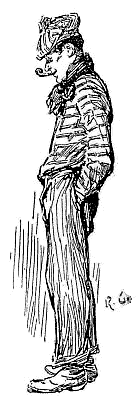
\includegraphics{images/sign410-sign-14.png}\end{center}

\noindent \begin{center}\noun{{}``I am off down the river, Watson,''
said he.}\end{center}
\end{figure}
{}``I am off down the river, Watson,'' said he. {}``I have been
turning it over in my mind, and I can see only one way out of it.
It is worth trying, at all events.''

{}``Surely I can come with you, then?'' said I.

{}``No; you can be much more useful if you will remain here as my
representative. I am loath to go, for it is quite on the cards that
some message may come during the day, though Wiggins was despondent
about it last night. I want you to open all notes and telegrams, and
to act on your own judgment if any news should come. Can I rely upon
you?''

{}``Most certainly.''

{}``I am afraid that you will not be able to wire to me, for I can
hardly tell yet where I may find myself. If I am in luck, however,
I may not be gone so very long. I shall have news of some sort or
other before I get back.''

I had heard nothing of him by breakfast-time. On opening the \emph{Standard},
however, I found that there was a fresh allusion to the business. 

\begin{quote} {}``With reference to the Upper Norwood tragedy,''
it remarked, {}``we have reason to believe that the matter promises
to be even more complex and mysterious than was originally supposed.
Fresh evidence has shown that it is quite impossible that Mr. Thaddeus
Sholto could have been in any way concerned in the matter. He and
the housekeeper, Mrs.\ Bernstone, were both released yesterday evening.
It is believed, however, that the police have a clue as to the real
culprits, and that it is being prosecuted by Mr.\ Athelney Jones,
of Scotland Yard, with all his well-known energy and sagacity. Further
arrests may be expected at any moment.''\end{quote}

{}``That is satisfactory so far as it goes,'' thought I. {}``Friend
Sholto is safe, at any rate. I wonder what the fresh clue may be;
though it seems to be a stereotyped form whenever the police have
made a blunder.''

I tossed the paper down upon the table, but at that moment my eye
caught an advertisement in the agony column. It ran in this way:

\begin{quote} {}``Lost.\mdsh{---}Whereas Mordecai Smith, boatman,
and his son, Jim, left Smith's Wharf at or about three o'clock last
Tuesday morning in the steam launch \emph{Aurora}, black with two
red stripes, funnel black with a white band, the sum of five pounds
will be paid to any one who can give information to Mrs.\ Smith,
at Smith's Wharf, or at \noun{221b} Baker Street, as to the whereabouts
of the said Mordecai Smith and the launch \emph{Aurora}.''\end{quote}

This was clearly Holmes's doing. The Baker Street address was enough
to prove that. It struck me as rather ingenious, because it might
be read by the fugitives without their seeing in it more than the
natural anxiety of a wife for her missing husband.

It was a long day. Every time that a knock came to the door, or a
sharp step passed in the street, I imagined that it was either Holmes
returning or an answer to his advertisement. I tried to read, but
my thoughts would wander off to our strange quest and to the ill-assorted
and villainous pair whom we were pursuing. Could there be, I wondered,
some radical flaw in my companion's reasoning. Might he be suffering
from some huge self-deception? Was it not possible that his nimble
and speculative mind had built up this wild theory upon faulty premises?
I had never known him to be wrong; and yet the keenest reasoner may
occasionally be deceived. He was likely, I thought, to fall into error
through the over-refinement of his logic,\mdsh{---}his preference
for a subtle and bizarre explanation when a plainer and more commonplace
one lay ready to his hand. Yet, on the other hand, I had myself seen
the evidence, and I had heard the reasons for his deductions. When
I looked back on the long chain of curious circumstances, many of
them trivial in themselves, but all tending in the same direction,
I could not disguise from myself that even if Holmes's explanation
were incorrect the true theory must be equally \emph{outré} and startling.

At three o'clock in the afternoon there was a loud peal at the bell,
an authoritative voice in the hall, and, to my surprise, no less a
person than Mr.\ Athelney Jones was shown up to me. Very different
was he, however, from the brusque and masterful professor of common
sense who had taken over the case so confidently at Upper Norwood.
His expression was downcast, and his bearing meek and even apologetic.

{}``Good-day, sir; good-day,'' said he. {}``Mr.\ Sherlock Holmes
is out, I understand.''

{}``Yes, and I cannot be sure when he will be back. But perhaps you
would care to wait. Take that chair and try one of these cigars.''

{}``Thank you; I don't mind if I do,'' said he, mopping his face
with a red bandanna handkerchief.

{}``And a whiskey-and-soda?''

{}``Well, half a glass. It is very hot for the time of year; and
I have had a good deal to worry and try me. You know my theory about
this Norwood case?''

{}``I remember that you expressed one.''

{}``Well, I have been obliged to reconsider it. I had my net drawn
tightly round Mr.\ Sholto, sir, when pop he went through a hole in
the middle of it. He was able to prove an alibi which could not be
shaken. From the time that he left his brother's room he was never
out of sight of some one or other. So it could not be he who climbed
over roofs and through trap-doors. It's a very dark case, and my professional
credit is at stake. I should be very glad of a little assistance.''

{}``We all need help sometimes,'' said I.

{}``Your friend Mr.\ Sherlock Holmes is a wonderful man, sir,''
said he, in a husky and confidential voice. {}``He's a man who is
not to be beat. I have known that young man go into a good many cases,
but I never saw the case yet that he could not throw a light upon.
He is irregular in his methods, and a little quick perhaps in jumping
at theories, but, on the whole, I think he would have made a most
promising officer, and I don't care who knows it. I have had a wire
from him this morning, by which I understand that he has got some
clue to this Sholto business. Here is the message.''

He took the telegram out of his pocket, and handed it to me. It was
dated from Poplar at twelve o'clock. \begin{quote} {}``Go to Baker
Street at once,'' it said. {}``If I have not returned, wait for
me. I am close on the track of the Sholto gang. You can come with
us to-night if you want to be in at the finish.''\end{quote}

{}``This sounds well. He has evidently picked up the scent again,''
said I.

{}``Ah, then he has been at fault too,'' exclaimed Jones, with evident
satisfaction. {}``Even the best of us are thrown off sometimes. Of
course this may prove to be a false alarm; but it is my duty as an
officer of the law to allow no chance to slip. But there is some one
at the door. Perhaps this is he.''

A heavy step was heard ascending the stair, with a great wheezing
and rattling as from a man who was sorely put to it for breath. Once
or twice he stopped, as though the climb were too much for him, but
at last he made his way to our door and entered. His appearance corresponded
to the sounds which we had heard. He was an aged man, clad in seafaring
garb, with an old pea-jacket buttoned up to his throat. His back was
bowed, his knees were shaky, and his breathing was painfully asthmatic.
As he leaned upon a thick oaken cudgel his shoulders heaved in the
effort to draw the air into his lungs. He had a colored scarf round
his chin, and I could see little of his face save a pair of keen dark
eyes, overhung by bushy white brows, and long gray side-whiskers.
Altogether he gave me the impression of a respectable master mariner
who had fallen into years and poverty.

{}``What is it, my man?'' I asked.

He looked about him in the slow methodical fashion of old age.

{}``Is Mr.\ Sherlock Holmes here?'' said he.

{}``No; but I am acting for him. You can tell me any message you
have for him.''

{}``It was to him himself I was to tell it,'' said he.

{}``But I tell you that I am acting for him. Was it about Mordecai
Smith's boat?''

{}``Yes. I knows well where it is. An' I knows where the men he is
after are. An' I knows where the treasure is. I knows all about it.''

{}``Then tell me, and I shall let him know.''

{}``It was to him I was to tell it,'' he repeated, with the petulant
obstinacy of a very old man.

{}``Well, you must wait for him.''

{}``No, no; I ain't goin' to lose a whole day to please no one. If
Mr.\ Holmes ain't here, then Mr.\ Holmes must find it all out for
himself. I don't care about the look of either of you, and I won't
tell a word.''

He shuffled towards the door, but Athelney Jones got in front of him.

{}``Wait a bit, my friend,'' said he. {}``You have important information,
and you must not walk off. We shall keep you, whether you like or
not, until our friend returns.''

The old man made a little run towards the door, but, as Athelney Jones
put his broad back up against it, he recognized the uselessness of
resistance.

{}``Pretty sort o' treatment this!''\ he cried, stamping his stick.
{}``I come here to see a gentleman, and you two, who I never saw
in my life, seize me and treat me in this fashion!''

{}``You will be none the worse,'' I said. {}``We shall recompense
you for the loss of your time. Sit over here on the sofa, and you
will not have long to wait.''

He came across sullenly enough, and seated himself with his face resting
on his hands. Jones and I resumed our cigars and our talk. Suddenly,
however, Holmes's voice broke in upon us.

{}``I think that you might offer me a cigar too,'' he said.

We both started in our chairs. There was Holmes sitting close to us
with an air of quiet amusement.

{}``Holmes!''\ I exclaimed. {}``You here! But where is the old
man?''

%
\begin{figure}[htbp]
\noindent \begin{center}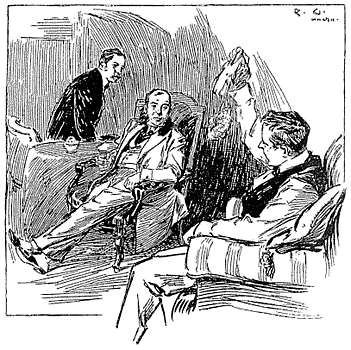
\includegraphics[%
  width=1\columnwidth]{images/sign410-sign-15.png}\end{center}

\noindent \begin{center}\noun{{}``Here is the old man,'' said
he, holding out a heap of white hair.}\end{center}
\end{figure}
{}``Here is the old man,'' said he, holding out a heap of white
hair. {}``Here he is,\mdsh{---}wig, whiskers, eyebrows, and all.
I thought my disguise was pretty good, but I hardly expected that
it would stand that test.''

{}``Ah, You rogue!''\ cried Jones, highly delighted. {}``You would
have made an actor, and a rare one. You had the proper workhouse cough,
and those weak legs of yours are worth ten pound a week. I thought
I knew the glint of your eye, though. You didn't get away from us
so easily, you see.''

{}``I have been working in that get-up all day,'' said he, lighting
his cigar. {}``You see, a good many of the criminal classes begin
to know me,\mdsh{---}especially since our friend here took to publishing
some of my cases: so I can only go on the war-path under some simple
disguise like this. You got my wire?''

{}``Yes; that was what brought me here.''

{}``How has your case prospered?''

{}``It has all come to nothing. I have had to release two of my prisoners,
and there is no evidence against the other two.''

{}``Never mind. We shall give you two others in the place of them.
But you must put yourself under my orders. You are welcome to all
the official credit, but you must act on the line that I point out.
Is that agreed?''

{}``Entirely, if you will help me to the men.''

{}``Well, then, in the first place I shall want a fast police-boat\mdsh{---}a
steam launch\mdsh{---}to be at the Westminster Stairs at seven o'clock.''

{}``That is easily managed. There is always one about there; but
I can step across the road and telephone to make sure.''

{}``Then I shall want two stanch men, in case of resistance.''

{}``There will be two or three in the boat. What else?''

{}``When we secure the men we shall get the treasure. I think that
it would be a pleasure to my friend here to take the box round to
the young lady to whom half of it rightfully belongs. Let her be the
first to open it.\mdsh{---} Eh, Watson?''

{}``It would be a great pleasure to me.''

{}``Rather an irregular proceeding,'' said Jones, shaking his head.
{}``However, the whole thing is irregular, and I suppose we must
wink at it. The treasure must afterwards be handed over to the authorities
until after the official investigation.''

{}``Certainly. That is easily managed. One other point. I should
much like to have a few details about this matter from the lips of
Jonathan Small himself. You know I like to work the detail of my cases
out. There is no objection to my having an unofficial interview with
him, either here in my rooms or elsewhere, as long as he is efficiently
guarded?''

{}``Well, you are master of the situation. I have had no proof yet
of the existence of this Jonathan Small. However, if you can catch
him I don't see how I can refuse you an interview with him.''

{}``That is understood, then?''

{}``Perfectly. Is there anything else?''

{}``Only that I insist upon your dining with us. It will be ready
in half an hour. I have oysters and a brace of grouse, with something
a little choice in white wines.\mdsh{---} Watson, you have never
yet recognized my merits as a housekeeper.''


\chapter*{\raggedright Chapter X. The End of the Islander}

\addcontentsline{toc}{chapter}{Chapter X. The End of the Islander}

\markboth{The Sign of the Four}{The End of the Islander}

Our meal was a merry one. Holmes could talk exceedingly well when
he chose, and that night he did choose. He appeared to be in a state
of nervous exaltation. I have never known him so brilliant. He spoke
on a quick succession of subjects,\mdsh{---}on miracle-plays, on
medieval pottery, on Stradivarius violins, on the Buddhism of Ceylon,
and on the war-ships of the future,\mdsh{---}handling each as though
he had made a special study of it. His bright humor marked the reaction
from his black depression of the preceding days. Athelney Jones proved
to be a sociable soul in his hours of relaxation, and face his dinner
with the air of a \emph{bon vivant}. For myself, I felt elated at
the thought that we were nearing the end of our task, and I caught
something of Holmes's gaiety. None of us alluded during dinner to
the cause which had brought us together.

When the cloth was cleared, Holmes glanced at this watch, and filled
up three glasses with port. {}``One bumper,'' said he, {}``to the
success of our little expedition. And now it is high time we were
off. Have you a pistol, Watson?''

{}``I have my old service-revolver in my desk.''

{}``You had best take it, then. It is well to be prepared. I see
that the cab is at the door. I ordered it for half-past six.''

It was a little past seven before we reached the Westminster wharf,
and found our launch awaiting us. Holmes eyed it critically.

{}``Is there anything to mark it as a police-boat?''

{}``Yes,\mdsh{---}that green lamp at the side.''

{}``Then take it off.''

The small change was made, we stepped on board, and the ropes were
cast off. Jones, Holmes, and I sat in the stern. There was one man
at the rudder, one to tend the engines, and two burly police-inspectors
forward.

{}``Where to?'' asked Jones.

{}``To the Tower. Tell them to stop opposite Jacobson's Yard.''

Our craft was evidently a very fast one. We shot past the long lines
of loaded barges as though they were stationary. Holmes smiled with
satisfaction as we overhauled a river steamer and left her behind
us.

{}``We ought to be able to catch anything on the river,'' he said.

{}``Well, hardly that. But there are not many launches to beat us.''

{}``We shall have to catch the \emph{Aurora}, and she has a name
for being a clipper. I will tell you how the land lies, Watson. You
recollect how annoyed I was at being balked by so small a thing?''

{}``Yes.''

{}``Well, I gave my mind a thorough rest by plunging into a chemical
analysis. One of our greatest statesmen has said that a change of
work is the best rest. So it is. When I had succeeded in dissolving
the hydrocarbon which I was at work at, I came back to our problem
of the Sholtos, and thought the whole matter out again. My boys had
been up the river and down the river without result. The launch was
not at any landing-stage or wharf, nor had it returned. Yet it could
hardly have been scuttled to hide their traces,\mdsh{---}though that
always remained as a possible hypothesis if all else failed. I knew
this man Small had a certain degree of low cunning, but I did not
think him capable of anything in the nature of delicate finesse. That
is usually a product of higher education. I then reflected that since
he had certainly been in London some time\mdsh{---}as we had evidence
that he maintained a continual watch over Pondicherry Lodge\mdsh{---}he
could hardly leave at a moment's notice, but would need some little
time, if it were only a day, to arrange his affairs. That was the
balance of probability, at any rate.''

{}``It seems to me to be a little weak,'' said I. {}``It is more
probable that he had arranged his affairs before ever he set out upon
his expedition.''

{}``No, I hardly think so. This lair of his would be too valuable
a retreat in case of need for him to give it up until he was sure
that he could do without it. But a second consideration struck me.
Jonathan Small must have felt that the peculiar appearance of his
companion, however much he may have top-coated him, would give rise
to gossip, and possibly be associated with this Norwood tragedy. He
was quite sharp enough to see that. They had started from their head-quarters
under cover of darkness, and he would wish to get back before it was
broad light. Now, it was past three o'clock, according to Mrs.\ Smith,
when they got the boat. It would be quite bright, and people would
be about in an hour or so. Therefore, I argued, they did not go very
far. They paid Smith well to hold his tongue, reserved his launch
for the final escape, and hurried to their lodgings with the treasure-box.
In a couple of nights, when they had time to see what view the papers
took, and whether there was any suspicion, they would make their way
under cover of darkness to some ship at Gravesend or in the Downs,
where no doubt they had already arranged for passages to America or
the Colonies.''

{}``But the launch? They could not have taken that to their lodgings.''

{}``Quite so. I argued that the launch must be no great way off,
in spite of its invisibility. I then put myself in the place of Small,
and looked at it as a man of his capacity would. He would probably
consider that to send back the launch or to keep it at a wharf would
make pursuit easy if the police did happen to get on his track. How,
then, could he conceal the launch and yet have her at hand when wanted?
I wondered what I should do myself if I were in his shoes. I could
only think of one way of doing it. I might land the launch over to
some boat-builder or repairer, with directions to make a trifling
change in her. She would then be removed to his shed or hard, and
so be effectually concealed, while at the same time I could have her
at a few hours' notice.''

{}``That seems simple enough.''

{}``It is just these very simple things which are extremely liable
to be overlooked. However, I determined to act on the idea. I started
at once in this harmless seaman's rig and inquired at all the yards
down the river. I drew blank at fifteen, but at the sixteenth\mdsh{---}Jacobson's\mdsh{---}I
learned that the \emph{Aurora} had been handed over to them two days
ago by a wooden-legged man, with some trivial directions as to her
rudder. `There ain't naught amiss with her rudder,' said the foreman.
`There she lies, with the red streaks.' At that moment who should
come down but Mordecai Smith, the missing owner? He was rather the
worse for liquor. I should not, of course, have known him, but he
bellowed out his name and the name of his launch. `I want her to-night
at eight o'clock,' said he,\mdsh{---}'eight o'clock sharp, mind,
for I have two gentlemen who won't be kept waiting.' They had evidently
paid him well, for he was very flush of money, chucking shillings
about to the men. I followed him some distance, but he subsided into
an ale-house: so I went back to the yard, and, happening to pick up
one of my boys on the way, I stationed him as a sentry over the launch.
He is to stand at water's edge and wave his handkerchief to us when
they start. We shall be lying off in the stream, and it will be a
strange thing if we do not take men, treasure, and all.''

{}``You have planned it all very neatly, whether they are the right
men or not,'' said Jones; {}``but if the affair were in my hands
I should have had a body of police in Jacobson's Yard, and arrested
them when they came down.''

{}``Which would have been never. This man Small is a pretty shrewd
fellow. He would send a scout on ahead, and if anything made him suspicious
lie snug for another week.''

{}``But you might have stuck to Mordecai Smith, and so been led to
their hiding-place,'' said I.

{}``In that case I should have wasted my day. I think that it is
a hundred to one against Smith knowing where they live. As long as
he has liquor and good pay, why should he ask questions? They send
him messages what to do. No, I thought over every possible course,
and this is the best.''

While this conversation had been proceeding, we had been shooting
the long series of bridges which span the Thames. As we passed the
City the last rays of the sun were gilding the cross upon the summit
of St.\ Paul's. It was twilight before we reached the Tower.

{}``That is Jacobson's Yard,'' said Holmes, pointing to a bristle
of masts and rigging on the Surrey side. {}``Cruise gently up and
down here under cover of this string of lighters.'' He took a pair
of night-glasses from his pocket and gazed some time at the shore.
{}``I see my sentry at his post,'' he remarked, {}``but no sign
of a handkerchief.''

{}``Suppose we go down-stream a short way and lie in wait for them,''
said Jones, eagerly. We were all eager by this time, even the policemen
and stokers, who had a very vague idea of what was going forward.

{}``We have no right to take anything for granted,'' Holmes answered.
{}``It is certainly ten to one that they go down-stream, but we cannot
be certain. From this point we can see the entrance of the yard, and
they can hardly see us. It will be a clear night and plenty of light.
We must stay where we are. See how the folk swarm over yonder in the
gaslight.''

{}``They are coming from work in the yard.''

{}``Dirty-looking rascals, but I suppose every one has some little
immortal spark concealed about him. You would not think it, to look
at them. There is no \emph{a priori} probability about it. A strange
enigma is man!''

{}``Some one calls him a soul concealed in an animal,'' I suggested.

{}``Winwood Reade is good upon the subject,'' said Holmes. {}``He
remarks that, while the individual man is an insoluble puzzle, in
the aggregate he becomes a mathematical certainty. You can, for example,
never foretell what any one man will do, but you can say with precision
what an average number will be up to. Individuals vary, but percentages
remain constant. So says the statistician. But do I see a handkerchief?
Surely there is a white flutter over yonder.''

{}``Yes, it is your boy,'' I cried. {}``I can see him plainly.''

{}``And there is the \emph{Aurora},'' exclaimed Holmes, {}``and
going like the devil! Full speed ahead, engineer. Make after that
launch with the yellow light. By heaven, I shall never forgive myself
if she proves to have the heels of us!''

She had slipped unseen through the yard-entrance and passed behind
two or three small craft, so that she had fairly got her speed up
before we saw her. Now she was flying down the stream, near in to
the shore, going at a tremendous rate. Jones looked gravely at her
and shook his head.

{}``She is very fast,'' he said. {}``I doubt if we shall catch
her.''

{}``We \textit{must} catch her!''\ cried Holmes, between his teeth.
{}``Heap it on, stokers! Make her do all she can! If we burn the
boat we must have them!''

%
\begin{figure}[htbp]
\noindent \begin{center}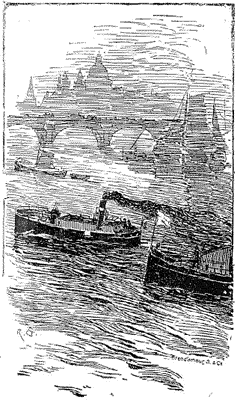
\includegraphics{images/sign410-sign-16.png}\end{center}

\noindent \begin{center}\noun{The furnaces roared, and the powerful
engines whizzed and clanked, like a great metallic heart.}\end{center}
\end{figure}
We were fairly after her now. The furnaces roared, and the powerful
engines whizzed and clanked, like a great metallic heart. Her sharp,
steep prow cut through the river-water and sent two rolling waves
to right and to left of us. With every throb of the engines we sprang
and quivered like a living thing. One great yellow lantern in our
bows threw a long, flickering funnel of light in front of us. Right
ahead a dark blur upon the water showed where the \emph{Aurora} lay,
and the swirl of white foam behind her spoke of the pace at which
she was going. We flashed past barges, steamers, merchant-vessels,
in and out, behind this one and round the other. Voices hailed us
out of the darkness, but still the \emph{Aurora} thundered on, and
still we followed close upon her track.

{}``Pile it on, men, pile it on!''\ cried Holmes, looking down
into the engine-room, while the fierce glow from below beat upon his
eager, aquiline face. {}``Get every pound of steam you can.''

{}``I think we gain a little,'' said Jones, with his eyes on the
\emph{Aurora}.

{}``I am sure of it,'' said I. {}``We shall be up with her in a
very few minutes.''

At that moment, however, as our evil fate would have it, a tug with
three barges in tow blundered in between us. It was only by putting
our helm hard down that we avoided a collision, and before we could
round them and recover our way the \emph{Aurora} had gained a good
two hundred yards. She was still, however, well in view, and the murky
uncertain twilight was setting into a clear starlit night. Our boilers
were strained to their utmost, and the frail shell vibrated and creaked
with the fierce energy which was driving us along. We had shot through
the Pool, past the West India Docks, down the long Deptford Reach,
and up again after rounding the Isle of Dogs. The dull blur in front
of us resolved itself now clearly enough into the dainty \emph{Aurora}.
Jones turned our search-light upon her, so that we could plainly see
the figures upon her deck. One man sat by the stern, with something
black between his knees over which he stooped. Beside him lay a dark
mass which looked like a Newfoundland dog. The boy held the tiller,
while against the red glare of the furnace I could see old Smith,
stripped to the waist, and shovelling coals for dear life. They may
have had some doubt at first as to whether we were really pursuing
them, but now as we followed every winding and turning which they
took there could no longer be any question about it. At Greenwich
we were about three hundred paces behind them. At Blackwall we could
not have been more than two hundred and fifty. I have coursed many
creatures in many countries during my checkered career, but never
did sport give me such a wild thrill as this mad, flying man-hunt
down the Thames. Steadily we drew in upon them, yard by yard. In the
silence of the night we could hear the panting and clanking of their
machinery. The man in the stern still crouched upon the deck, and
his arms were moving as though he were busy, while every now and then
he would look up and measure with a glance the distance which still
separated us. Nearer we came and nearer. Jones yelled to them to stop.
We were not more than four boat's lengths behind them, both boats
flying at a tremendous pace. It was a clear reach of the river, with
Barking Level upon one side and the melancholy Plumstead Marshes upon
the other. At our hail the man in the stern sprang up from the deck
and shook his two clinched fists at us, cursing the while in a high,
cracked voice. He was a good-sized, powerful man, and as he stood
poising himself with legs astride I could see that from the thigh
downwards there was but a wooden stump upon the right side. At the
sound of his strident, angry cries there was movement in the huddled
bundle upon the deck. It straightened itself into a little black man\mdsh{---}the
smallest I have ever seen\mdsh{---}with a great, misshapen head and
a shock of tangled, dishevelled hair. Holmes had already drawn his
revolver, and I whipped out mine at the sight of this savage, distorted
creature. He was wrapped in some sort of dark ulster or blanket, which
left only his face exposed; but that face was enough to give a man
a sleepless night. Never have I seen features so deeply marked with
all bestiality and cruelty. His small eyes glowed and burned with
a sombre light, and his thick lips were writhed back from his teeth,
which grinned and chattered at us with a half animal fury.

{}``Fire if he raises his hand,'' said Holmes, quietly. We were
within a boat's-length by this time, and almost within touch of our
quarry. I can see the two of them now as they stood, the white man
with his legs far apart, shrieking out curses, and the unhallowed
dwarf with his hideous face, and his strong yellow teeth gnashing
at us in the light of our lantern.

%
\begin{figure}[htbp]
\noindent \begin{center}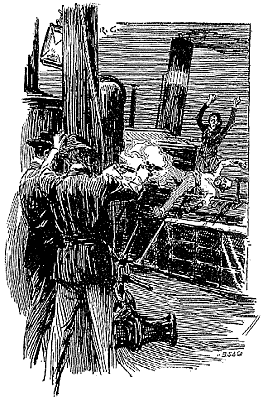
\includegraphics{images/sign410-sign-17.png}\end{center}

\noindent \begin{center}\noun{Our pistols rang out together.}\end{center}
\end{figure}
It was well that we had so clear a view of him. Even as we looked
he plucked out from under his covering a short, round piece of wood,
like a school-ruler, and clapped it to his lips. Our pistols rang
out together. He whirled round, threw up his arms, and with a kind
of choking cough fell sideways into the stream. I caught one glimpse
of his venomous, menacing eyes amid the white swirl of the waters.
At the same moment the wooden-legged man threw himself upon the rudder
and put it hard down, so that his boat made straight in for the southern
bank, while we shot past her stern, only clearing her by a few feet.
We were round after her in an instant, but she was already nearly
at the bank. It was a wild and desolate place, where the moon glimmered
upon a wide expanse of marsh-land, with pools of stagnant water and
beds of decaying vegetation. The launch with a dull thud ran up upon
the mud-bank, with her bow in the air and her stern flush with the
water. The fugitive sprang out, but his stump instantly sank its whole
length into the sodden soil. In vain he struggled and writhed. Not
one step could he possibly take either forwards or backwards. He yelled
in impotent rage, and kicked frantically into the mud with his other
foot, but his struggles only bored his wooden pin the deeper into
the sticky bank. When we brought our launch alongside he was so firmly
anchored that it was only by throwing the end of a rope over his shoulders
that we were able to haul him out, and to drag him, like some evil
fish, over our side. The two Smiths, father and son, sat sullenly
in their launch, but came aboard meekly enough when commanded. The
\emph{Aurora} herself we hauled off and made fast to our stern. A
solid iron chest of Indian workmanship stood upon the deck. This,
there could be no question, was the same that had contained the ill-omened
treasure of the Sholtos. There was no key, but it was of considerable
weight, so we transferred it carefully to our own little cabin. As
we steamed slowly up-stream again, we flashed our search-light in
every direction, but there was no sign of the Islander. Somewhere
in the dark ooze at the bottom of the Thames lie the bones of that
strange visitor to our shores.

{}``See here,'' said Holmes, pointing to the wooden hatchway. {}``We
were hardly quick enough with our pistols.'' There, sure enough,
just behind where we had been standing, stuck one of those murderous
darts which we knew so well. It must have whizzed between us at the
instant that we fired. Holmes smiled at it and shrugged his shoulders
in his easy fashion, but I confess that it turned me sick to think
of the horrible death which had passed so close to us that night.


\chapter*{\raggedright Chapter XI. The Great Agra Treasure}

\addcontentsline{toc}{chapter}{Chapter XI. The Great Agra Treasure}

\markboth{The Sign of the Four}{The Great Agra Treasure}

Our captive sat in the cabin opposite to the iron box which he had
done so much and waited so long to gain. He was a sunburned, reckless-eyed
fellow, with a net-work of lines and wrinkles all over his mahogany
features, which told of a hard, open-air life. There was a singular
prominence about his bearded chin which marked a man who was not to
be easily turned from his purpose. His age may have been fifty or
thereabouts, for his black, curly hair was thickly shot with gray.
%
\begin{figure}[htbp]
\noindent \begin{center}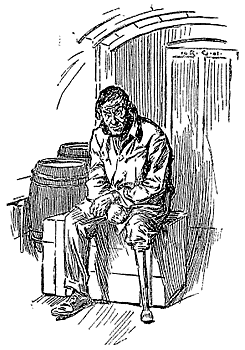
\includegraphics{images/sign410-sign-18.png}\end{center}

\noindent \begin{center}\noun{He sat now with his handcuffed hands
upon his lap.}\end{center}
\end{figure}
His face in repose was not an unpleasing one, though his heavy brows
and aggressive chin gave him, as I had lately seen, a terrible expression
when moved to anger. He sat now with his handcuffed hands upon his
lap, and his head sunk upon his breast, while he looked with his keen,
twinkling eyes at the box which had been the cause of his ill-doings.
It seemed to me that there was more sorrow than anger in his rigid
and contained countenance. Once he looked up at me with a gleam of
something like humor in his eyes.

{}``Well, Jonathan Small,'' said Holmes, lighting a cigar, {}``I
am sorry that it has come to this.''

{}``And so am I, sir,'' he answered, frankly. {}``I don't believe
that I can swing over the job. I give you my word on the book that
I never raised hand against Mr.\ Sholto. It was that little hell-hound
Tonga who shot one of his cursed darts into him. I had no part in
it, sir. I was as grieved as if it had been my blood-relation. I welted
the little devil with the slack end of the rope for it, but it was
done, and I could not undo it again.''

{}``Have a cigar,'' said Holmes; {}``and you had best take a pull
out of my flask, for you are very wet. How could you expect so small
and weak a man as this black fellow to overpower Mr.\ Sholto and
hold him while you were climbing the rope?''

{}``You seem to know as much about it as if you were there, sir.
The truth is that I hoped to find the room clear. I knew the habits
of the house pretty well, and it was the time when Mr. Sholto usually
went down to his supper. I shall make no secret of the business. The
best defence that I can make is just the simple truth. Now, if it
had been the old major I would have swung for him with a light heart.
I would have thought no more of knifing him than of smoking this cigar.
But it's cursed hard that I should be lagged over this young Sholto,
with whom I had no quarrel whatever.''

{}``You are under the charge of Mr.\ Athelney Jones, of Scotland
Yard. He is going to bring you up to my rooms, and I shall ask you
for a true account of the matter. You must make a clean breast of
it, for if you do I hope that I may be of use to you. I think I can
prove that the poison acts so quickly that the man was dead before
ever you reached the room.''

{}``That he was, sir. I never got such a turn in my life as when
I saw him grinning at me with his head on his shoulder as I climbed
through the window. It fairly shook me, sir. I'd have half killed
Tonga for it if he had not scrambled off. That was how he came to
leave his club, and some of his darts too, as he tells me, which I
dare say helped to put you on our track; though how you kept on it
is more than I can tell. I don't feel no malice against you for it.
But it does seem a queer thing,'' he added, with a bitter smile,
{}``that I who have a fair claim to nigh upon half a million of money
should spend the first half of my life building a breakwater in the
Andamans, and am like to spend the other half digging drains at Dartmoor.
It was an evil day for me when first I clapped eyes upon the merchant
Achmet and had to do with the Agra treasure, which never brought anything
but a curse yet upon the man who owned it. To him it brought murder,
to Major Sholto it brought fear and guilt, to me it has meant slavery
for life.''

At this moment Athelney Jones thrust his broad face and heavy shoulders
into the tiny cabin. {}``Quite a family party,'' he remarked. {}``I
think I shall have a pull at that flask, Holmes. Well, I think we
may all congratulate each other. Pity we didn't take the other alive;
but there was no choice. I say, Holmes, you must confess that you
cut it rather fine. It was all we could do to overhaul her.''

{}``All is well that ends well,'' said Holmes. {}``But I certainly
did not know that the \emph{Aurora} was such a clipper.''

{}``Smith says she is one of the fastest launches on the river, and
that if he had had another man to help him with the engines we should
never have caught her. He swears he knew nothing of this Norwood business.''

{}``Neither he did,'' cried our prisoner,\mdsh{---}``not a word.
I chose his launch because I heard that she was a flier. We told him
nothing, but we paid him well, and he was to get something handsome
if we reached our vessel, the \emph{Esmeralda}, at Gravesend, outward
bound for the Brazils.''

{}``Well, if he has done no wrong we shall see that no wrong comes
to him. If we are pretty quick in catching our men, we are not so
quick in condemning them.'' It was amusing to notice how the consequential
Jones was already beginning to give himself airs on the strength of
the capture. From the slight smile which played over Sherlock Holmes's
face, I could see that the speech had not been lost upon him.

{}``We will be at Vauxhall Bridge presently,'' said Jones, {}``and
shall land you, Dr.\ Watson, with the treasure-box. I need hardly
tell you that I am taking a very grave responsibility upon myself
in doing this. It is most irregular; but of course an agreement is
an agreement. I must, however, as a matter of duty, send an inspector
with you, since you have so valuable a charge. You will drive, no
doubt?''

{}``Yes, I shall drive.''

{}``It is a pity there is no key, that we may make an inventory first.
You will have to break it open. Where is the key, my man?''

{}``At the bottom of the river,'' said Small, shortly.

{}``Hum! There was no use your giving this unnecessary trouble. We
have had work enough already through you. However, doctor, I need
not warn you to be careful. Bring the box back with you to the Baker
Street rooms. You will find us there, on our way to the station.''

They landed me at Vauxhall, with my heavy iron box, and with a bluff,
genial inspector as my companion. A quarter of an hour's drive brought
us to Mrs.\ Cecil Forrester's. The servant seemed surprised at so
late a visitor. Mrs.\ Cecil Forrester was out for the evening, she
explained, and likely to be very late. Miss Morstan, however, was
in the drawing-room: so to the drawing-room I went, box in hand, leaving
the obliging inspector in the cab.

She was seated by the open window, dressed n some sort of white diaphanous
material, with a little touch of scarlet at the neck and waist. The
soft light of a shaded lamp fell upon her as she leaned back in the
basket chair, playing over her sweet, grave face, and tinting with
a dull, metallic sparkle the rich coils of her luxuriant hair. One
white arm and hand drooped over the side of the chair, and her whole
pose and figure spoke of an absorbing melancholy. At the sound of
my foot-fall she sprang to her feet, however, and a bright flush of
surprise and of pleasure colored her pale cheeks.

{}``I heard a cab drive up,'' she said. {}``I thought that Mrs.
Forrester had come back very early, but I never dreamed that it might
be you. What news have you brought me?''

{}``I have brought something better than news,'' said I, putting
down the box upon the table and speaking jovially and boisterously,
though my heart was heavy within me. {}``I have brought you something
which is worth all the news in the world. I have brought you a fortune.''

She glanced at iron box. {}``Is that the treasure, then?'' she asked,
coolly enough.

{}``Yes, this is the great Agra treasure. Half of it is yours and
half is Thaddeus Sholto's. You will have a couple of hundred thousand
each. Think of that! An annuity of ten thousand pounds. There will
be few richer young ladies in England. Is it not glorious?''

I think that I must have been rather overacting my delight, and that
she detected a hollow ring in my congratulations, for I saw her eyebrows
rise a little, and she glanced at me curiously.

{}``If I have it,'' said she, {}``I owe it to you.''

{}``No, no,'' I answered, {}``not to me, but to my friend Sherlock
Holmes. With all the will in the world, I could never have followed
up a clue which has taxed even his analytical genius. As it was, we
very nearly lost it at the last moment.''

{}``Pray sit down and tell me all about it, Dr.\ Watson,'' said
she.

I narrated briefly what had occurred since I had seen her last,\mdsh{---}Holmes's
new method of search, the discovery of the \emph{Aurora}, the appearance
of Athelney Jones, our expedition in the evening, and the wild chase
down the Thames. She listened with parted lips and shining eyes to
my recital of our adventures. When I spoke of the dart which had so
narrowly missed us, she turned so white that I feared that she was
about to faint.

{}``It is nothing,'' she said, as I hastened to pour her out some
water. {}``I am all right again. It was a shock to me to hear that
I had placed my friends in such horrible peril.''

{}``That is all over,'' I answered. {}``It was nothing. I will
tell you no more gloomy details. Let us turn to something brighter.
There is the treasure. What could be brighter than that? I got leave
to bring it with me, thinking that it would interest you to be the
first to see it.''

{}``It would be of the greatest interest to me,'' she said. There
was no eagerness in her voice, however. It had struck her, doubtless,
that it might seem ungracious upon her part to be indifferent to a
prize which had cost so much to win.

{}``What a pretty box!''\ she said, stooping over it. This is Indian
work, I suppose?''

{}``Yes; it is Benares metal-work.''

And so heavy!''\ she exclaimed, trying to raise it. {}``The box
alone must be of some value. Where is the key?''

{}``Small threw it into the Thames,'' I answered. {}``I must borrow
Mrs.\ Forrester's poker.'' There was in the front a thick and broad
hasp, wrought in the image of a sitting Buddha. Under this I thrust
the end of the poker and twisted it outward as a lever. The hasp sprang
open with a loud snap. With trembling fingers I flung back the lid.
We both stood gazing in astonishment. The box was empty!

No wonder that it was heavy. The iron-work was two-thirds of an inch
thick all round. It was massive, well made, and solid, like a chest
constructed to carry things of great price, but not one shred or crumb
of metal or jewelry lay within it. It was absolutely and completely
empty.

{}``The treasure is lost,'' said Miss Morstan, calmly.

As I listened to the words and realized what they meant, a great shadow
seemed to pass from my soul. I did not know how this Agra treasure
had weighed me down, until now that it was finally removed. It was
selfish, no doubt, disloyal, wrong, but I could realize nothing save
that the golden barrier was gone from between us. {}``Thank God!''\ I
ejaculated from my very heart.

She looked at me with a quick, questioning smile. {}``Why do you
say that?''\ she asked.

{}``Because you are within my reach again,'' I said, taking her
hand. She did not withdraw it. {}``Because I love you, Mary, as truly
as ever a man loved a woman. Because this treasure, these riches,
sealed my lips. Now that they are gone I can tell you how I love you.
That is why I said, `Thank God.'''

%
\begin{figure}[htbp]
\noindent \begin{center}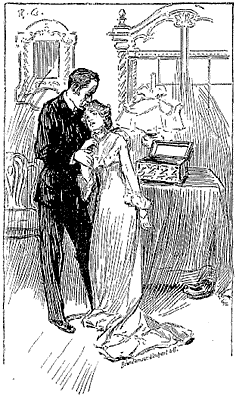
\includegraphics{images/sign410-sign-19.png}\end{center}

\noindent \begin{center}\noun{{}``Then I say, `Thank God,' too.''}\end{center}
\end{figure}
{}``Then I say, `Thank God,' too,'' she whispered, as I drew her
to my side. Whoever had lost a treasure, I knew that night that I
had gained one.


\chapter*{\raggedright Chapter XII. The Strange Story of Jonathan Small}

\addcontentsline{toc}{chapter}{Chapter XII. The Strange Story of\\
Jonathan Small}

\markboth{The Sign of the Four}{The Strange Story of Jonathan Small}

A very patient man was that inspector in the cab, for it was a weary
time before I rejoined him. His face clouded over when I showed him
the empty box.

{}``There goes the reward!'' said he, gloomily. {}``Where there
is no money there is no pay. This night's work would have been worth
a tenner each to Sam Brown and me if the treasure had been there.''

{}``Mr.\ Thaddeus Sholto is a rich man,'' I said. {}``He will
see that you are rewarded, treasure or no.''

The inspector shook his head despondently, however. {}``It's a bad
job,'' he repeated; {}``and so Mr.\ Athelney Jones will think.''

His forecast proved to be correct, for the detective looked blank
enough when I got to Baker Street and showed him the empty box. They
had only just arrived, Holmes, the prisoner, and he, for they had
changed their plans so far as to report themselves at a station upon
the way. My companion lounged in his arm-chair with his usual listless
expression, while Small sat stolidly opposite to him with his wooden
leg cocked over his sound one. As I exhibited the empty box he leaned
back in his chair and laughed aloud.

{}``This is your doing, Small,'' said Athelney Jones, angrily.

{}``Yes, I have put it away where you shall never lay hand upon it,''
he cried, exultantly. {}``It is my treasure; and if I can't have
the loot I'll take darned good care that no one else does. I tell
you that no living man has any right to it, unless it is three men
who are in the Andaman convict-barracks and myself. I know now that
I cannot have the use of it, and I know that they cannot. I have acted
all through for them as much as for myself. It's been the sign of
four with us always. Well I know that they would have had me do just
what I have done, and throw the treasure into the Thames rather than
let it go to kith or kin of Sholto or of Morstan. It was not to make
them rich that we did for Achmet. You'll find the treasure where the
key is, and where little Tonga is. When I saw that your launch must
catch us, I put the loot away in a safe place. There are no rupees
for you this journey.''

{}``You are deceiving us, Small,'' said Athelney Jones, sternly.
{}``If you had wished to throw the treasure into the Thames it would
have been easier for you to have thrown box and all.''

{}``Easier for me to throw, and easier for you to recover,'' he
answered, with a shrewd, sidelong look. {}``The man that was clever
enough to hunt me down is clever enough to pick an iron box from the
bottom of a river. Now that they are scattered over five miles or
so, it may be a harder job. It went to my heart to do it, though.
I was half mad when you came up with us. However, there's no good
grieving over it. I've had ups in my life, and I've had downs, but
I've learned not to cry over spilled milk.''

{}``This is a very serious matter, Small,'' said the detective.
{}``If you had helped justice, instead of thwarting it in this way,
you would have had a better chance at your trial.''

{}``Justice!'' snarled the ex-convict. {}``A pretty justice! Whose
loot is this, if it is not ours? Where is the justice that I should
give it up to those who have never earned it? Look how I have earned
it! Twenty long years in that fever-ridden swamp, all day at work
under the mangrove-tree, all night chained up in the filthy convict-huts,
bitten by mosquitoes, racked with ague, bullied by every cursed black-faced
policeman who loved to take it out of a white man. That was how I
earned the Agra treasure; and you talk to me of justice because I
cannot bear to feel that I have paid this price only that another
may enjoy it! I would rather swing a score of times, or have one of
Tonga's darts in my hide, than live in a convict's cell and feel that
another man is at his ease in a palace with the money that should
be mine.'' Small had dropped his mask of stoicism, and all this came
out in a wild whirl of words, while his eyes blazed, and the handcuffs
clanked together with the impassioned movement of his hands. I could
understand, as I saw the fury and the passion of the man, that it
was no groundless or unnatural terror which had possessed Major Sholto
when he first learned that the injured convict was upon his track.

'You forget that we know nothing of all this,'' said Holmes quietly.
{}``We have not heard your story, and we cannot tell how far justice
may originally have been on your side.''

{}``Well, sir, you have been very fair-spoken to me, though I can
see that I have you to thank that I have these bracelets upon my wrists.
Still, I bear no grudge for that. It is all fair and above-board.
If you want to hear my story I have no wish to hold it back. What
I say to you is God's truth, every word of it. Thank you; you can
put the glass beside me here, and I'll put my lips to it if I am dry.

{}``I am a Worcestershire man myself,\mdsh{---}born near Pershore.
I dare say you would find a heap of Smalls living there now if you
were to look. I have often thought of taking a look round there, but
the truth is that I was never much of a credit to the family, and
I doubt if they would be so very glad to see me. They were all steady,
chapel-going folk, small farmers, well known and respected over the
country-side, while I was always a bit of a rover. At last, however,
when I was about eighteen, I gave them no more trouble, for I got
into a mess over a girl, and could only get out of it again by taking
the queen's shilling and joining the 3d Buffs, which was just starting
for India.

{}``I wasn't destined to do much soldiering, however. I had just
got past the goose-step, and learned to handle my musket, when I was
fool enough to go swimming in the Ganges. Luckily for me, my company
sergeant, John Holder, was in the water at the same time, and he was
one of the finest swimmers in the service. A crocodile took me, just
as I was half-way across, and nipped off my right leg as clean as
a surgeon could have done it, just above the knee. What with the shock
and the loss of blood, I fainted, and should have drowned if Holder
had not caught hold of me and paddled for the bank. I was five months
in hospital over it, and when at last I was able to limp out of it
with this timber toe strapped to my stump I found myself invalided
out of the army and unfitted for any active occupation.

{}``I was, as you can imagine, pretty down on my luck at this time,
for I was a useless cripple though not yet in my twentieth year. However,
my misfortune soon proved to be a blessing in disguise. A man named
Abelwhite, who had come out there as an indigo-planter, wanted an
overseer to look after his coolies and keep them up to their work.
He happened to be a friend of our colonel's, who had taken an interest
in me since the accident. To make a long story short, the colonel
recommended me strongly for the post and, as the work was mostly to
be done on horseback, my leg was no great obstacle, for I had enough
knee left to keep good grip on the saddle. What I had to do was to
ride over the plantation, to keep an eye on the men as they worked,
and to report the idlers. The pay was fair, I had comfortable quarters,
and altogether I was content to spend the remainder of my life in
indigo-planting. Mr.\ Abelwhite was a kind man, and he would often
drop into my little shanty and smoke a pipe with me, for white folk
out there feel their hearts warm to each other as they never do here
at home.

{}``Well, I was never in luck's way long. Suddenly, without a note
of warning, the great mutiny broke upon us. One month India lay as
still and peaceful, to all appearance, as Surrey or Kent; the next
there were two hundred thousand black devils let loose, and the country
was a perfect hell. Of course you know all about it, gentlemen,\mdsh{---}a
deal more than I do, very like, since reading is not in my line. I
only know what I saw with my own eyes. Our plantation was at a place
called Muttra, near the border of the Northwest Provinces. Night after
night the whole sky was alight with the burning bungalows, and day
after day we had small companies of Europeans passing through our
estate with their wives and children, on their way to Agra, where
were the nearest troops. Mr.\ Abelwhite was an obstinate man. He
had it in his head that the affair had been exaggerated, and that
it would blow over as suddenly as it had sprung up. There he sat on
his veranda, drinking whiskey-pegs and smoking cheroots, while the
country was in a blaze about him. Of course we stuck by him, I and
Dawson, who, with his wife, used to do the book-work and the managing.
Well, one fine day the crash came. I had been away on a distant plantation,
and was riding slowly home in the evening, when my eye fell upon something
all huddled together at the bottom of a steep nullah. I rode down
to see what it was, and the cold struck through my heart when I found
it was Dawson's wife, all cut into ribbons, and half eaten by jackals
and native dogs. A little further up the road Dawson himself was lying
on his face, quite dead, with an empty revolver in his hand and four
Sepoys lying across each other in front of him. I reined up my horse,
wondering which way I should turn, but at that moment I saw thick
smoke curling up from Abelwhite's bungalow and the flames beginning
to burst through the roof. I knew then that I could do my employer
no good, but would only throw my own life away if I meddled in the
matter. %
\begin{figure}[htbp]
\noindent \begin{center}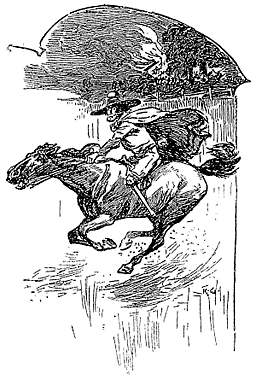
\includegraphics{images/sign410-sign-20.png}\end{center}

\noindent \begin{center}\noun{I broke away across the paddy-fields.}\end{center}
\end{figure}
From where I stood I could see hundreds of the black fiends, with
their red coats still on their backs, dancing and howling round the
burning house. Some of them pointed at me, and a couple of bullets
sang past my head; so I broke away across the paddy-fields, and found
myself late at night safe within the walls at Agra.

{}``As it proved, however, there was no great safety there, either.
The whole country was up like a swarm of bees. Wherever the English
could collect in little bands they held just the ground that their
guns commanded. Everywhere else they were helpless fugitives. It was
a fight of the millions against the hundreds; and the cruellest part
of it was that these men that we fought against, foot, horse, and
gunners, were our own picked troops, whom we had taught and trained,
handling our own weapons, and blowing our own bugle-calls. At Agra
there were the 3d Bengal Fusiliers, some Sikhs, two troops of horse,
and a battery of artillery. A volunteer corps of clerks and merchants
had been formed, and this I joined, wooden leg and all. We went out
to meet the rebels at Shahgunge early in July, and we beat them back
for a time, but our powder gave out, and we had to fall back upon
the city. Nothing but the worst news came to us from every side,\mdsh{---}which
is not to be wondered at, for if you look at the map you will see
that we were right in the heart of it. Lucknow is rather better than
a hundred miles to the east, and Cawnpore about as far to the south.
From every point on the compass there was nothing but torture and
murder and outrage.

{}``The city of Agra is a great place, swarming with fanatics and
fierce devil-worshippers of all sorts. Our handful of men were lost
among the narrow, winding streets. Our leader moved across the river,
therefore, and took up his position in the old fort at Agra. I don't
know if any of you gentlemen have ever read or heard anything of that
old fort. It is a very queer place,\mdsh{---}the queerest that ever
I was in, and I have been in some rum corners, too. First of all,
it is enormous in size. I should think that the enclosure must be
acres and acres. There is a modern part, which took all our garrison,
women, children, stores, and everything else, with plenty of room
over. But the modern part is nothing like the size of the old quarter,
where nobody goes, and which is given over to the scorpions and the
centipedes. It is all full of great deserted halls, and winding passages,
and long corridors twisting in and out, so that it is easy enough
for folk to get lost in it. For this reason it was seldom that any
one went into it, though now and again a party with torches might
go exploring.

{}``The river washes along the front of the old fort, and so protects
it, but on the sides and behind there are many doors, and these had
to be guarded, of course, in the old quarter as well as in that which
was actually held by our troops. We were short-handed, with hardly
men enough to man the angles of the building and to serve the guns.
It was impossible for us, therefore, to station a strong guard at
every one of the innumerable gates. What we did was to organize a
central guard-house in the middle of the fort, and to leave each gate
under the charge of one white man and two or three natives. I was
selected to take charge during certain hours of the night of a small
isolated door upon the southwest side of the building. Two Sikh troopers
were placed under my command, and I was instructed if anything went
wrong to fire my musket, when I might rely upon help coming at once
from the central guard. As the guard was a good two hundred paces
away, however, and as the space between was cut up into a labyrinth
of passages and corridors, I had great doubts as to whether they could
arrive in time to be of any use in case of an actual attack.

{}``Well, I was pretty proud at having this small command given me,
since I was a raw recruit, and a game-legged one at that. For two
nights I kept the watch with my Punjaubees. They were tall, fierce-looking
chaps, Mahomet Singh and Abdullah Khan by name, both old fighting-men
who had borne arms against us at Chilian-wallah. They could talk English
pretty well, but I could get little out of them. They preferred to
stand together and jabber all night in their queer Sikh lingo. For
myself, I used to stand outside the gate-way, looking down on the
broad, winding river and on the twinkling lights of the great city.
The beating of drums, the rattle of tomtoms, and the yells and howls
of the rebels, drunk with opium and with bang, were enough to remind
us all night of our dangerous neighbors across the stream. Every two
hours the officer of the night used to come round to all the posts,
to make sure that all was well.

{}``The third night of my watch was dark and dirty, with a small,
driving rain. It was dreary work standing in the gate-way hour after
hour in such weather. I tried again and again to make my Sikhs talk,
but without much success. At two in the morning the rounds passed,
and broke for a moment the weariness of the night. Finding that my
companions would not be led into conversation, I took out my pipe,
and laid down my musket to strike the match. %
\begin{figure}[htbp]
\noindent \begin{center}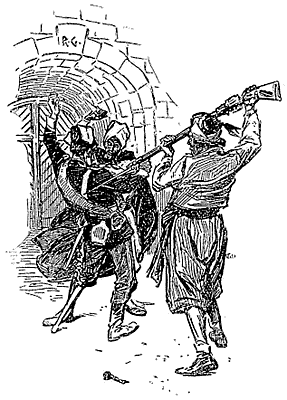
\includegraphics{images/sign410-sign-21.png}\end{center}

\noindent \begin{center}\noun{In an instant the two Sikhs were upon
me.}\end{center}
\end{figure}
In an instant the two Sikhs were upon me. One of them snatched my
firelock up and levelled it at my head, while the other held a great
knife to my throat and swore between his teeth that he would plunge
it into me if I moved a step.

{}``My first thought was that these fellows were in league with the
rebels, and that this was the beginning of an assault. If our door
were in the hands of the Sepoys the place must fall, and the women
and children be treated as they were in Cawnpore. Maybe you gentlemen
think that I am just making out a case for myself, but I give you
my word that when I thought of that, though I felt the point of the
knife at my throat, I opened my mouth with the intention of giving
a scream, if it was my last one, which might alarm the main guard.
The man who held me seemed to know my thoughts; for, even as I braced
myself to it, he whispered, `Don't make a noise. The fort is safe
enough. There are no rebel dogs on this side of the river.' There
was the ring of truth in what he said, and I knew that if I raised
my voice I was a dead man. I could read it in the fellow's brown eyes.
I waited, therefore, in silence, to see what it was that they wanted
from me.

{}```Listen to me, Sahib,' said the taller and fiercer of the pair,
the one whom they called Abdullah Khan. `You must either be with us
now or you must be silenced forever. The thing is too great a one
for us to hesitate. Either you are heart and soul with us on your
oath on the cross of the Christians, or your body this night shall
be thrown into the ditch and we shall pass over to our brothers in
the rebel army. There is no middle way. Which is it to be, death or
life? We can only give you three minutes to decide, for the time is
passing, and all must be done before the rounds come again.'

{}```How can I decide?'\ said I. `You have not told me what you
want of me. But I tell you now that if it is anything against the
safety of the fort I will have no truck with it, so you can drive
home your knife and welcome.'

{}```It is nothing against the fort,' said he. `We only ask you to
do that which your countrymen come to this land for. We ask you to
be rich. If you will be one of us this night, we will swear to you
upon the naked knife, and by the threefold oath which no Sikh was
ever known to break, that you shall have your fair share of the loot.
A quarter of the treasure shall be yours. We can say no fairer.'

{}```But what is the treasure, then?' I asked. `I am as ready to
be rich as you can be, if you will but show me how it can be done.'

{}```You will swear, then,' said he, `by the bones of your father,
by the honor of your mother, by the cross of your faith, to raise
no hand and speak no word against us, either now or afterwards?'

{}```I will swear it,' I answered, `provided that the fort is not
endangered.'

{}```Then my comrade and I will swear that you shall have a quarter
of the treasure which shall be equally divided among the four of us.'

{}```There are but three,' said I.

{}```No; Dost Akbar must have his share. We can tell the tale to
you while we await them. Do you stand at the gate, Mahomet Singh,
and give notice of their coming. The thing stands thus, Sahib, and
I tell it to you because I know that an oath is binding upon a Feringhee,
and that we may trust you. Had you been a lying Hindoo, though you
had sworn by all the gods in their false temples, your blood would
have been upon the knife, and your body in the water. But the Sikh
knows the Englishman, and the Englishman knows the Sikh. Hearken,
then, to what I have to say.

{}```There is a rajah in the northern provinces who has much wealth,
though his lands are small. Much has come to him from his father,
and more still he has set by himself, for he is of a low nature and
hoards his gold rather than spend it. When the troubles broke out
he would be friends both with the lion and the tiger,\mdsh{---}with
the Sepoy and with the Company's Raj. Soon, however, it seemed to
him that the white men's day was come, for through all the land he
could hear of nothing but of their death and their overthrow. Yet,
being a careful man, he made such plans that, come what might, half
at least of his treasure should be left to him. That which was in
gold and silver he kept by him in the vaults of his palace, but the
most precious stones and the choicest pearls that he had he put in
an iron box, and sent it by a trusty servant who, under the guise
of a merchant, should take it to the fort at Agra, there to lie until
the land is at peace. Thus, if the rebels won he would have his money,
but if the Company conquered his jewels would be saved to him. Having
thus divided his hoard, he threw himself into the cause of the Sepoys,
since they were strong upon his borders. By doing this, mark you,
Sahib, his property becomes the due of those who have been true to
their salt.

{}```This pretended merchant, who travels under the name of Achmet,
is now in the city of Agra, and desires to gain his way into the fort.
He has with him as travelling-companion my foster-brother Dost Akbar,
who knows his secret. Dost Akbar has promised this night to lead him
to a side-postern of the fort, and has chosen this one for his purpose.
Here he will come presently, and here he will find Mahomet Singh and
myself awaiting him. The place is lonely, and none shall know of his
coming. The world shall know of the merchant Achmet no more, but the
great treasure of the rajah shall be divided among us. What say you
to it, Sahib?'

{}``In Worcestershire the life of a man seems a great and a sacred
thing; but it is very different when there is fire and blood all round
you and you have been used to meeting death at every turn. Whether
Achmet the merchant lived or died was a thing as light as air to me,
but at the talk about the treasure my heart turned to it, and I thought
of what I might do in the old country with it, and how my folk would
stare when they saw their ne'er-do-well coming back with his pockets
full of gold moidores. I had, therefore, already made up my mind.
Abdullah Khan, however, thinking that I hesitated, pressed the matter
more closely.

{}```Consider, Sahib,' said he, `that if this man is taken by the
commandant he will be hung or shot, and his jewels taken by the government,
so that no man will be a rupee the better for them. Now, since we
do the taking of him, why should we not do the rest as well? The jewels
will be as well with us as in the Company's coffers. There will be
enough to make every one of us rich men and great chiefs. No one can
know about the matter, for here we are cut off from all men. What
could be better for the purpose? Say again, then, Sahib, whether you
are with us, or if we must look upon you as an enemy.'

{}```I am with you heart and soul,' said I.

{}```It is well,' he answered, handing me back my firelock. `You
see that we trust you, for your word, like ours, is not to be broken.
We have now only to wait for my brother and the merchant.'

{}```Does your brother know, then, of what you will do?' I asked.

{}```The plan is his. He has devised it. We will go to the gate and
share the watch with Mahomet Singh.'

{}```he rain was still falling steadily, for it was just the beginning
of the wet season. Brown, heavy clouds were drifting across the sky,
and it was hard to see more than a stone-cast. A deep moat lay in
front of our door, but the water was in places nearly dried up, and
it could easily be crossed. It was strange to me to be standing there
with those two wild Punjaubees waiting for the man who was coming
to his death.

{}``Suddenly my eye caught the glint of a shaded lantern at the other
side of the moat. It vanished among the mound-heaps, and then appeared
again coming slowly in our direction.

{}```Here they are!'\ I exclaimed.

{}```You will challenge him, Sahib, as usual,' whispered Abdullah.
`Give him no cause for fear. Send us in with him, and we shall do
the rest while you stay here on guard. Have the lantern ready to uncover,
that we may be sure that it is indeed the man.'

{}``The light had flickered onwards, now stopping and now advancing,
until I could see two dark figures upon the other side of the moat.
I let them scramble down the sloping bank, splash through the mire,
and climb half-way up to the gate, before I challenged them.

{}```Who goes there?'\ said I, in a subdued voice.

{}```Friends,' came the answer. I uncovered my lantern and threw
a flood of light upon them. The first was an enormous Sikh, with a
black beard which swept nearly down to his cummerbund. Outside of
a show I have never seen so tall a man. The other was a little, fat,
round fellow, with a great yellow turban, and a bundle in his hand,
done up in a shawl. He seemed to be all in a quiver with fear, for
his hands twitched as if he had the ague, and his head kept turning
to left and right with two bright little twinkling eyes, like a mouse
when he ventures out from his hole. It gave me the chills to think
of killing him, but I thought of the treasure, and my heart set as
hard as a flint within me. When he saw my white face he gave a little
chirrup of joy and came running up towards me.

{}```Your protection, Sahib,' he pant\-ed,\mdsh{---}`your protection
for the unhappy merchant Achmet. I have travelled across Rajpootana
that I might seek the shelter of the fort at Agra. I have been robbed
and beaten and abused because I have been the friend of the Company.
It is a blessed night this when I am once more in safety,\mdsh{---}I
and my poor possessions.'

{}```What have you in the bundle?' I asked.

{}```An iron box,' he answered, `which contains one or two little
family matters which are of no value to others, but which I should
be sorry to lose. Yet I am not a beggar; and I shall reward you, young
Sahib, and your governor also, if he will give me the shelter I ask.'

{}``I could not trust myself to speak longer with the man. The more
I looked at his fat, frightened face, the harder did it seem that
we should slay him in cold blood. It was best to get it over.

{}```Take him to the main guard,' said I.\  The two Sikhs closed
in upon him on each side, and the giant walked behind, while they
marched in through the dark gate-way. Never was a man so compassed
round with death. I remained at the gate-way with the lantern.

{}``I could hear the measured tramp of their footsteps sounding through
the lonely corridors. Suddenly it ceased, and I heard voices, and
a scuffle, with the sound of blows. A moment later there came, to
my horror, a rush of footsteps coming in my direction, with the loud
breathing of a running man. %
\begin{figure}[htbp]
\noindent \begin{center}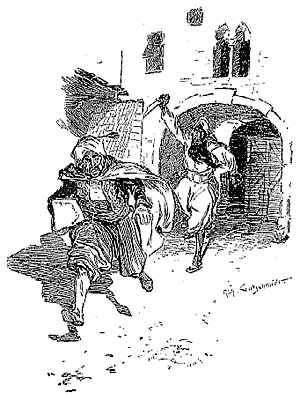
\includegraphics[%
  width=1\columnwidth]{images/sign410-sign-22.png}\end{center}

\noindent \begin{center}\noun{And close at his heels, bounding like
a tiger, the great black-bearded Sikh, with a knife flashing in his
hand.}\end{center}
\end{figure}
I turned my lantern down the long, straight passage, and there was
the fat man, running like the wind, with a smear of blood across his
face, and close at his heels, bounding like a tiger, the great black-bearded
Sikh, with a knife flashing in his hand. I have never seen a man run
so fast as that little merchant. He was gaining on the Sikh, and I
could see that if he once passed me and got to the open air he would
save himself yet. My heart softened to him, but again the thought
of his treasure turned me hard and bitter. I cast my firelock between
his legs as he raced past, and he rolled twice over like a shot rabbit.
Ere he could stagger to his feet the Sikh was upon him, and buried
his knife twice in his side. The man never uttered moan nor moved
muscle, but lay where he had fallen. I think myself that he may have
broken his neck with the fall. You see, gentlemen, that I am keeping
my promise. I am telling you every work of the business just exactly
as it happened, whether it is in my favor or not.''

He stopped, and held out his manacled hands for the whiskey-and-water
which Holmes had brewed for him. For myself, I confess that I had
now conceived the utmost horror of the man, not only for this cold-blooded
business in which he had been concerned, but even more for the somewhat
flippant and careless way in which he narrated it. Whatever punishment
was in store for him, I felt that he might expect no sympathy from
me. Sherlock Holmes and Jones sat with their hands upon their knees,
deeply interested in the story, but with the same disgust written
upon their faces. He may have observed it, for there was a touch of
defiance in his voice and manner as he proceeded.

{}``It was all very bad, no doubt,'' said he. {}``I should like
to know how many fellows in my shoes would have refused a share of
this loot when they knew that they would have their throats cut for
their pains. Besides, it was my life or his when once he was in the
fort. If he had got out, the whole business would come to light, and
I should have been court-martialled and shot as likely as not; for
people were not very lenient at a time like that.''

{}``Go on with your story,'' said Holmes, shortly.

{}``Well, we carried him in, Abdullah, Akbar, and I.\  A fine weight
he was, too, for all that he was so short. Mahomet Singh was left
to guard the door. We took him to a place which the Sikhs had already
prepared. It was some distance off, where a winding passage leads
to a great empty hall, the brick walls of which were all crumbling
to pieces. The earth floor had sunk in at one place, making a natural
grave, so we left Achmet the merchant there, having first covered
him over with loose bricks. This done, we all went back to the treasure.

{}``It lay where he had dropped it when he was first attacked. The
box was the same which now lies open upon your table. A key was hung
by a silken cord to that carved handle upon the top. We opened it,
and the light of the lantern gleamed upon a collection of gems such
as I have read of and thought about when I was a little lad at Pershore.
It was blinding to look upon them. When we had feasted our eyes we
took them all out and made a list of them. There were one hundred
and forty-three diamonds of the first water, including one which has
been called, I believe, `the Great Mogul' and is said to be the second
largest stone in existence. Then there were ninety-seven very fine
emeralds, and one hundred and seventy rubies, some of which, however,
were small. There were forty carbuncles, two hundred and ten sapphires,
sixty-one agates, and a great quantity of beryls, onyxes, cats'-eyes,
turquoises, and other stones, the very names of which I did not know
at the time, though I have become more familiar with them since. Besides
this, there were nearly three hundred very fine pearls, twelve of
which were set in a gold coronet. By the way, these last had been
taken out of the chest and were not there when I recovered it.

{}``After we had counted our treasures we put them back into the
chest and carried them to the gate-way to show them to Mahomet Singh.
Then we solemnly renewed our oath to stand by each other and be true
to our secret. We agreed to conceal our loot in a safe place until
the country should be at peace again, and then to divide it equally
among ourselves. There was no use dividing it at present, for if gems
of such value were found upon us it would cause suspicion, and there
was no privacy in the fort nor any place where we could keep them.
We carried the box, therefore, into the same hall where we had buried
the body, and there, under certain bricks in the best-preserved wall,
we made a hollow and put our treasure. We made careful note of the
place, and next day I drew four plans, one for each of us, and put
the sign of the four of us at the bottom, for we had sworn that we
should each always act for all, so that none might take advantage.
That is an oath that I can put my hand to my heart and swear that
I have never broken.

{}``Well, there's no use my telling you gentlemen what came of the
Indian mutiny. After Wilson took Delhi and Sir Colin relieved Lucknow
the back of the business was broken. Fresh troops came pouring in,
and Nana Sahib made himself scarce over the frontier. A flying column
under Colonel Greathed came round to Agra and cleared the Pandies
away from it. Peace seemed to be settling upon the country, and we
four were beginning to hope that the time was at hand when we might
safely go off with our shares of the plunder. In a moment, however,
our hopes were shattered by our being arrested as the murderers of
Achmet.

{}``It came about in this way. When the rajah put his jewels into
the hands of Achmet he did it because he knew that he was a trusty
man. They are suspicious folk in the East, however: so what does this
rajah do but take a second even more trusty servant and set him to
play the spy upon the first? This second man was ordered never to
let Achmet out of his sight, and he followed him like his shadow.
He went after him that night and saw him pass through the doorway.
Of course he thought he had taken refuge in the fort, and applied
for admission there himself next day, but could find no trace of Achmet.
This seemed to him so strange that he spoke about it to a sergeant
of guides, who brought it to the ears of the commandant. A thorough
search was quickly made, and the body was discovered. Thus at the
very moment that we thought that all was safe we were all four seized
and brought to trial on a charge of murder,\mdsh{---}three of us
because we had held the gate that night, and the fourth because he
was known to have been in the company of the murdered man. Not a word
about the jewels came out at the trial, for the rajah had been deposed
and driven out of India: so no one had any particular interest in
them. The murder, however, was clearly made out, and it was certain
that we must all have been concerned in it. The three Sikhs got penal
servitude for life, and I was condemned to death, though my sentence
was afterwards commuted into the same as the others.

{}``It was rather a queer position that we found ourselves in then.
There we were all four tied by the leg and with precious little chance
of ever getting out again, while we each held a secret which might
have put each of us in a palace if we could only have made use of
it. It was enough to make a man eat his heart out to have to stand
the kick and the cuff of every petty jack-in-office, to have rice
to eat and water to drink, when that gorgeous fortune was ready for
him outside, just waiting to be picked up. It might have driven me
mad; but I was always a pretty stubborn one, so I just held on and
bided my time.

{}``At last it seemed to me to have come. I was changed from Agra
to Madras, and from there to Blair Island in the Andamans. There are
very few white convicts at this settlement, and, as I had behaved
well from the first, I soon found myself a sort of privileged person.
I was given a hut in Hope Town, which is a small place on the slopes
of Mount Harriet, and I was left pretty much to myself. It is a dreary,
fever-stricken place, and all beyond our little clearings was infested
with wild cannibal natives, who were ready enough to blow a poisoned
dart at us if they saw a chance. There was digging, and ditching,
and yam-planting, and a dozen other things to be done, so we were
busy enough all day; though in the evening we had a little time to
ourselves. Among other things, I learned to dispense drugs for the
surgeon, and picked up a smattering of his knowledge. All the time
I was on the lookout for a chance of escape; but it is hundreds of
miles from any other land, and there is little or no wind in those
seas: so it was a terribly difficult job to get away.

{}``The surgeon, Dr.\ Somerton, was a fast, sporting young chap,
and the other young officers would meet in his rooms of an evening
and play cards. The surgery, where I used to make up my drugs, was
next to his sitting-room, with a small window between us. Often, if
I felt lonesome, I used to turn out the lamp in the surgery, and then,
standing there, I could hear their talk and watch their play. I am
fond of a hand at cards myself, and it was almost as good as having
one to watch the others. There was Major Sholto, Captain Morstan,
and Lieutenant Bromley Brown, who were in command of the native troops,
and there was the surgeon himself, and two or three prison-officials,
crafty old hands who played a nice sly safe game. A very snug little
party they used to make.

{}``Well, there was one thing which very soon struck me, and that
was that the soldiers used always to lose and the civilians to win.
Mind, I don't say that there was anything unfair, but so it was. These
prison-chaps had done little else than play cards ever since they
had been at the Andamans, and they knew each other's game to a point,
while the others just played to pass the time and threw their cards
down anyhow. Night after night the soldiers got up poorer men, and
the poorer they got the more keen they were to play. Major Sholto
was the hardest hit. He used to pay in notes and gold at first, but
soon it came to notes of hand and for big sums. He sometimes would
win for a few deals, just to give him heart, and then the luck would
set in against him worse than ever. All day he would wander about
as black as thunder, and he took to drinking a deal more than was
good for him.

{}``One night he lost even more heavily than usual. I was sitting
in my hut when he and Captain Morstan came stumbling along on the
way to their quarters. They were bosom friends, those two, and never
far apart. The major was raving about his losses.

{}```It's all up, Morstan,' he was saying, as they passed my hut.
`I shall have to send in my papers. I am a ruined man.'

{}```Nonsense, old chap!' said the other, slapping him upon the shoulder.
`I've had a nasty facer myself, but\mdsh{---}' That was all I could
hear, but it was enough to set me thinking.

A couple of days later Major Sholto was strolling on the beach: so
I took the chance of speaking to him.

{}```I wish to have your advice, major,' said I.

{}```Well, Small, what is it?' he asked, taking his cheroot from
his lips.

{}```I wanted to ask you, sir,' said I, `who is the proper person
to whom hidden treasure should be handed over. I know where half a
million worth lies, and, as I cannot use it myself, I thought perhaps
the best thing that I could do would be to hand it over to the proper
authorities, and then perhaps they would get my sentence shortened
for me.'

{}```Half a million, Small?' he gasped, looking hard at me to see
if I was in earnest.

{}```Quite that, sir,\mdsh{---}in jewels and pearls. It lies there
ready for any one. And the queer thing about it is that the real owner
is outlawed and cannot hold property, so that it belongs to the first
comer.'

{}```To government, Small,' he stam\-mer\-ed,\mdsh{---}`to government.'
But he said it in a halting fashion, and I knew in my heart that I
had got him.

{}```You think, then, sir, that I should give the information to
the Governor-General?' said I, quietly.

{}```Well, well, you must not do anything rash, or that you might
repent. Let me hear all about it, Small. Give me the facts.'

{}``I told him the whole story, with small changes so that he could
not identify the places. When I had finished he stood stock still
and full of thought. I could see by the twitch of his lip that there
was a struggle going on within him.

{}```This is a very important matter, Small,' he said, at last. `You
must not say a word to any one about it, and I shall see you again
soon.'

{}``Two nights later he and his friend Captain Morstan came to my
hut in the dead of the night with a lantern.

%
\begin{figure}[htbp]
\noindent \begin{center}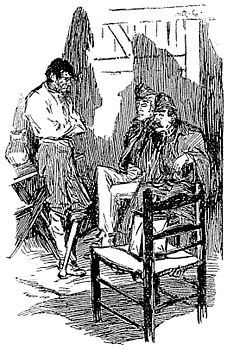
\includegraphics{images/sign410-sign-23.png}\end{center}

\noindent \begin{center}\noun{`I want you just to let Captain Morstan
hear that story from your own lips, Small,' said he.}\end{center}
\end{figure}
{}```I want you just to let Captain Morstan hear that story from
your own lips, Small,' said he.

{}``I repeated it as I had told it before.

{}```It rings true, eh?' said he. `It's good enough to act upon?'

{}``Captain Morstan nodded.

{}```Look here, Small,' said the major. `We have been talking it
over, my friend here and I, and we have come to the conclusion that
this secret of yours is hardly a government matter, after all, but
is a private concern of your own, which of course you have the power
of disposing of as you think best. Now, the question is, what price
would you ask for it? We might be inclined to take it up, and at least
look into it, if we could agree as to terms.' He tried to speak in
a cool, careless way, but his eyes were shining with excitement and
greed.

{}```Why, as to that, gentlemen,' I answered, trying also to be cool,
but feeling as excited as he did, `there is only one bargain which
a man in my position can make. I shall want you to help me to my freedom,
and to help my three companions to theirs. We shall then take you
into partnership, and give you a fifth share to divide between you.'

{}```Hum!' said he. `A fifth share! That is not very tempting.'

{}```It would come to fifty thousand apiece,' said I.

{}``'But how can we gain your freedom? You know very well that you
ask an impossibility.'

{}```Nothing of the sort,' I answered. `I have thought it all out
to the last detail. The only bar to our escape is that we can get
no boat fit for the voyage, and no provisions to last us for so long
a time. There are plenty of little yachts and yawls at Calcutta or
Madras which would serve our turn well. Do you bring one over. We
shall engage to get aboard her by night, and if you will drop us on
any part of the Indian coast you will have done your part of the bargain.'

{}```If there were only one,' he said.

{}```None or all,' I answered. `We have sworn it. The four of us
must always act together.'

{}```You see, Morstan,' said he, `Small is a man of his word. He
does not flinch from his friend. I think we may very well trust him.'

{}```It's a dirty business,' the other answered. `Yet, as you say,
the money would save our commissions handsomely.'

{}```Well, Small,' said the major, `we must, I suppose, try and meet
you. We must first, of course, test the truth of your story. Tell
me where the box is hid, and I shall get leave of absence and go back
to India in the monthly relief-boat to inquire into the affair.'

{}```Not so fast,' said I, growing colder as he got hot. `I must
have the consent of my three comrades. I tell you that it is four
or none with us.'

{}```Nonsense!' he broke in. `What have three black fellows to do
with our agreement?'

{}```Black or blue,' said I, `they are in with me, and we all go
together.'

{}``Well, the matter ended by a second meeting, at which Mahomet
Singh, Abdullah Khan, and Dost Akbar were all present. We talked the
matter over again, and at last we came to an arrangement. We were
to provide both the officers with charts of the part of the Agra fort
and mark the place in the wall where the treasure was hid. Major Sholto
was to go to India to test our story. If he found the box he was to
leave it there, to send out a small yacht provisioned for a voyage,
which was to lie off Rutland Island, and to which we were to make
our way, and finally to return to his duties. Captain Morstan was
then to apply for leave of absence, to meet us at Agra, and there
we were to have a final division of the treasure, he taking the major's
share as well as his own. All this we sealed by the most solemn oaths
that the mind could think or the lips utter. I sat up all night with
paper and ink, and by the morning I had the two charts all ready,
signed with the sign of four,\mdsh{---}that is, of Abdullah, Akbar,
Mahomet, and myself.

{}``Well, gentlemen, I weary you with my long story, and I know that
my friend Mr.\ Jones is impatient to get me safely stowed in chokey.
I'll make it as short as I can. The villain Sholto went off to India,
but he never came back again. Captain Morstan showed me his name among
a list of passengers in one of the mail-boats very shortly afterwards.
His uncle had died, leaving him a fortune, and he had left the army,
yet he could stoop to treat five men as he had treated us. Morstan
went over to Agra shortly afterwards, and found, as we expected, that
the treasure was indeed gone. The scoundrel had stolen it all, without
carrying out one of the conditions on which we had sold him the secret.\ 
From that day I lived only for vengeance. I thought of it by day and
I nursed it by night. It became an overpowering, absorbing passion
with me. I cared nothing for the law,\mdsh{---}nothing for the gallows.
To escape, to track down Sholto, to have my hand upon his throat,\mdsh{---}that
was my one thought. Even the Agra treasure had come to be a smaller
thing in my mind than the slaying of Sholto.

{}``Well, I have set my mind on many things in this life, and never
one which I did not carry out. But it was weary years before my time
came. I have told you that I had picked up something of medicine.
One day when Dr.\ Somerton was down with a fever a little Andaman
Islander was picked up by a convict-gang in the woods. He was sick
to death, and had gone to a lonely place to die. I took him in hand,
though he was as venomous as a young snake, and after a couple of
months I got him all right and able to walk. He took a kind of fancy
to me then, and would hardly go back to his woods, but was always
hanging about my hut. I learned a little of his lingo from him, and
this made him all the fonder of me.

{}``Tonga\mdsh{---}for that was his name\mdsh{---}was a fine boatman,
and owned a big, roomy canoe of his own. When I found that he was
devoted to me and would do anything to serve me, I saw my chance of
escape. I talked it over with him. He was to bring his boat round
on a certain night to an old wharf which was never guarded, and there
he was to pick me up. I gave him directions to have several gourds
of water and a lot of yams, cocoa-nuts, and sweet potatoes.

{}``He was stanch and true, was little Tonga. No man ever had a more
faithful mate. At the night named he had his boat at the wharf. As
it chanced, however, there was one of the convict-guard down there,\mdsh{---}a
vile Pathan who had never missed a chance of insulting and injuring
me. I had always vowed vengeance, and now I had my chance. It was
as if fate had placed him in my way that I might pay my debt before
I left the island. He stood on the bank with his back to me, and his
carbine on his shoulder. I looked abut for a stone to beat out his
brains with, but none could I see. Then a queer thought came into
my head and showed me where I could lay my hand on a weapon. I sat
down in the darkness and unstrapped my wooden leg. With three long
hops I was on him. He put his carbine to his shoulder, but I struck
him full, and knocked the whole front of his skull in. You can see
the split in the wood now where I hit him. We both went down together,
for I could not keep my balance, but when I got up I found him still
lying quiet enough. I made for the boat, and in an hour we were well
out at sea. Tonga had brought all his earthly possessions with him,
his arms and his gods. Among other things, he had a long bamboo spear,
and some Andaman cocoa-nut matting, with which I make a sort of sail.
For ten days we were beating about, trusting to luck, and on the eleventh
we were picked up by a trader which was going from Singapore to Jiddah
with a cargo of Malay pilgrims. They were a rum crowd, and Tonga and
I soon managed to settle down among them. They had one very good quality:
they let you alone and asked no questions.

{}``Well, if I were to tell you all the adventures that my little
chum and I went through, you would not thank me, for I would have
you here until the sun was shining. Here and there we drifted about
the world, something always turning up to keep us from London. All
the time, however, I never lost sight of my purpose. I would dream
of Sholto at night. A hundred times I have killed him in my sleep.
At last, however, some three or four years ago, we found ourselves
in England. I had no great difficulty in finding where Sholto lived,
and I set to work to discover whether he had realized the treasure,
or if he still had it. I made friends with someone who could help
me,\mdsh{---}I name no names, for I don't want to get any one else
in a hole,\mdsh{---}and I soon found that he still had the jewels.
Then I tried to get at him in many ways; but he was pretty sly, and
had always two prize-fighters, besides his sons and his \emph{khitmutgar},
on guard over him.

{}``One day, however, I got word that he was dying. I hurried at
once to the garden, mad that he should slip out of my clutches like
that, and, looking through the window, I saw him lying in his bed,
with his sons on each side of him. I'd have come through and taken
my chance with the three of them, only even as I looked at him his
jaw dropped, and I knew that he was gone. I got into his room that
same night, though, and I searched his papers to see if there was
any record of where he had hidden our jewels. There was not a line,
however: so I came away, bitter and savage as a man could be. Before
I left I bethought me that if I ever met my Sikh friends again it
would be a satisfaction to know that I had left some mark of our hatred:
so I scrawled down the sign of the four of us, as it had been on the
chart, and I pinned it on his bosom. It was too much that he should
be taken to the grave without some token from the men whom he had
robbed and befooled.

{}``We earned a living at this time by my exhibiting poor Tonga at
fairs and other such places as the black cannibal. He would eat raw
meat and dance his war-dance: so we always had a hatful of pennies
after a day's work. I still heard all the news from Pondicherry Lodge,
and for some years there was no news to hear, except that they were
hunting for the treasure. At last, however, came what we had waited
for so long. The treasure had been found. It was up at the top of
the house, in Mr. Bartholomew Sholto's chemical laboratory. I came
at once and had a look at the place, but I could not see how with
my wooden leg I was to make my way up to it. I learned, however, about
a trap-door in the roof, and also about Mr.\ Sholto's supper-hour.
It seemed to me that I could manage the thing easily through Tonga.
I brought him out with me with a long rope wound round his waist.
He could climb like a cat, and he soon made his way through the roof,
but, as ill luck would have it, Bartholomew Sholto was still in the
room, to his cost. Tonga thought he had done something very clever
in killing him, for when I came up by the rope I found him strutting
about as proud as a peacock. Very much surprised was he when I made
at him with the rope's end and cursed him for a little blood-thirsty
imp. I took the treasure-box and let it down, and then slid down myself,
having first left the sign of the four upon the table, to show that
the jewels had come back at last to those who had most right to them.
Tonga then pulled up the rope, closed the window, and made off the
way that he had come.

{}``I don't know that I have anything else to tell you. I had heard
a waterman speak of the speed of Smith's launch the \emph{Aurora},
so I thought she would be a handy craft for our escape. I engaged
with old Smith, and was to give him a big sum if he got us safe to
our ship. He knew, no doubt, that there was some screw loose, but
he was not in our secrets. All this is the truth, and if I tell it
to you, gentlemen, it is not to amuse you,\mdsh{---}for you have
not done me a very good turn,\mdsh{---}but it is because I believe
the best defence I can make is just to hold back nothing, but let
all the wold know how badly I have myself been served by Major Sholto,
and how innocent I am of the death of his son.''

{}``A very remarkable account,'' said Sherlock Holmes. {}``A fitting
wind-up to an extremely interesting case. There is nothing at all
new to me in the latter part of your narrative, except that you brought
your own rope. That I did not know. By the way, I had hoped that Tonga
had lost all his darts; yet he managed to shoot one at us in the boat.''

{}``He had lost them all, sir, except the one which was in his blow-pipe
at the time.''

{}``Ah, of course,'' said Holmes. {}``I had not thought of that.''

{}``Is there any other point which you would like to ask about?''
asked the convict, affably.

{}``I think not, thank you,'' my companion answered.

{}``Well, Holmes,'' said Athelney Jones, {}``You are a man to be
humored, and we all know that you are a connoisseur of crime, but
duty is duty, and I have gone rather far in doing what you and your
friend asked me. I shall feel more at ease when we have our story-teller
here safe under lock and key. The cab still waits, and there are two
inspectors down-stairs. %
\begin{figure}[htbp]
\noindent \begin{center}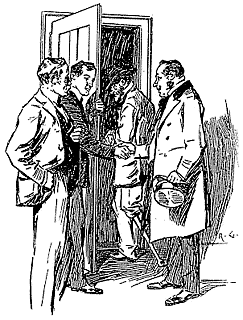
\includegraphics{images/sign410-sign-24.png}\end{center}

\noindent \begin{center}\noun{I am much obliged to you both for
your assistance.}\end{center}
\end{figure}
I am much obliged to you both for your assistance. Of course you will
be wanted at the trial. Good-night to you.''

{}``Good-night, gentlemen both,'' said Jon\-a\-than Small.

{}``You first, Small,'' remarked the wary Jones as they left the
room. {}``I'll take particular care that you don't club me with your
wooden leg, whatever you may have done to the gentleman at the Andaman
Isles.''

{}``Well, and there is the end of our little drama,'' I remarked,
after we had set some time smoking in silence. {}``I fear that it
may be the last investigation in which I shall have the chance of
studying your methods. Miss Morstan has done me the honor to accept
me as a husband in prospective.''

He gave a most dismal groan. {}``I feared as much,'' said he. {}``I
really cannot congratulate you.''

I was a little hurt. {}``Have you any reason to be dissatisfied with
my choice?'' I asked.

{}``Not at all. I think she is one of the most charming young ladies
I ever met, and might have been most useful in such work as we have
been doing. She had a decided genius that way: witness the way in
which she preserved that Agra plan from all the other papers of her
father. But love is an emotional thing, and whatever is emotional
is opposed to that true cold reason which I place above all things.
I should never marry myself, lest I bias my judgment.''

{}``I trust,'' said I, laughing, {}``that my judgment may survive
the ordeal. But you look weary.''

{}``Yes, the reaction is already upon me. I shall be as limp as a
rag for a week.''

{}``Strange,'' said I, {}``how terms of what in another man I should
call laziness alternate with your fits of splendid energy and vigor.''

{}``Yes,'' he answered, {}``there are in me the makings of a very
fine loafer and also of a pretty spry sort of fellow. I often think
of those lines of old Goethe,\mdsh{---}

\begin{quote}
\emph{Schade dass die Natur nur} \textit{einen} \emph{Mensch aus Dir
schuf, Denn zum wuerdigen Mann war und zum Schelmen der Stoff.}
\end{quote}
By the way, \emph{a propos} of this Norwood business, you see that
they had, as I surmised, a confederate in the house, who could be
none other than Lal Rao, the butler: so Jones actually has the undivided
honor of having caught one fish in his great haul.''

{}``The division seems rather unfair,'' I remarked. {}``You have
done all the work in this business. I get a wife out of it, Jones
gets the credit, pray what remains for you?''

{}``For me,'' said Sherlock Holmes, {}``there still remains the
cocaine-bottle.'' And he stretched his long white hand up for it.
\end{document}
